%	PACKAGES AND OTHER DOCUMENT CONFIGURATIONS
%-----------------------------------------------------------------------
\documentclass[11pt,fleqn]{book} % Default font size and left-justified equations
%--------------------------------------------------------------
%	VARIOUS REQUIRED PACKAGES AND CONFIGURATIONS
%--------------------------------------------------------------
\usepackage[top=3cm,bottom=3cm,left=3cm,right=3cm,headsep=10pt,a4paper]{geometry} % Page margins
\usepackage{graphicx} % Required for including pictures
%\graphicspath{{Pictures/}} % Specifies the directory where pictures are stored
\usepackage{lipsum} % Inserts dummy text
\usepackage{tikz} % Required for drawing custom shapes
\usepackage[spanish]{babel} % English language/hyphenation
\usepackage{enumitem} % Customize lists
\setlist{nolistsep} % Reduce spacing between bullet points and numbered lists
\usepackage{booktabs} % Required for nicer horizontal rules in tables
\usepackage{xcolor} % Required for specifying colors by name
\definecolor{ocre}{RGB}{243,102,25} % Define the orange color used for highlighting throughout the book
%--------------------------------------------------------------
%	FONTS
%--------------------------------------------------------------
%\usepackage{avant} % Use the Avantgarde font for headings
\usepackage{times} % Use the Times font for headings
\usepackage{mathptmx} % Use the Adobe Times Roman as the default text font together with math symbols from the Sym­bol, Chancery and Com­puter Modern fonts
\usepackage{microtype} % Slightly tweak font spacing for aesthetics
\usepackage[utf8]{inputenc} % Required for including letters with accents
\usepackage[T1]{fontenc} % Use 8-bit encoding that has 256 glyphs
%--------------------------------------------------------------
%	BIBLIOGRAPHY AND INDEX
%--------------------------------------------------------------
\usepackage[style=alphabetic,citestyle=numeric,sorting=nyt,sortcites=true,autopunct=true,babel=hyphen,hyperref=true,abbreviate=false,backref=true,backend=biber]{biblatex}
\addbibresource{bibliografia.bib} % BibTeX bibliography file
\defbibheading{bibempty}{}
\usepackage{calc} % For simpler calculation - used for spacing the index letter headings correctly
\usepackage{makeidx} % Required to make an index
\makeindex % Tells LaTeX to create the files required for indexing
%---------------------------------------------------------
%	MAIN TABLE OF CONTENTS
%---------------------------------------------------------
\usepackage{titletoc} % Required for manipulating the table of contents
\contentsmargin{0cm} % Removes the default margin
% Part text styling
\titlecontents{part}[0cm]
{\addvspace{-200pt}\centering\large\bfseries}% ubicacion de tabla de contenido
{}
{}
{}
% Chapter text styling
\titlecontents{chapter}[1.25cm] % Indentation
{\addvspace{12pt}\large\sffamily\bfseries} % Spacing and font options for chapters
{\color{ocre!60}\contentslabel[\Large\thecontentslabel]{1.25cm}\color{ocre}} % Chapter number
{\color{ocre}}  
{\color{ocre!60}\normalsize\;\titlerule*[.5pc]{.}\;\thecontentspage} % Page number
% Section text styling
\titlecontents{section}[1.25cm] % Indentation
{\addvspace{.5pt}\sffamily\bfseries} % Spacing and font options for sections
{\contentslabel[\thecontentslabel]{1.25cm}} % Section number
{}
{\hfill\color{black}\thecontentspage} % Page number
[]
% Subsection text styling
\titlecontents{subsection}[1.25cm] % Indentation
{\addvspace{1pt}\sffamily\small} % Spacing and font options for subsections
{\contentslabel[\thecontentslabel]{1.25cm}} % Subsection number
{}
{\ \titlerule*[.5pc]{.}\;\thecontentspage} % Page number
[]
%---------------------------------------------------------
%	PAGE HEADERS
%---------------------------------------------------------
\usepackage{fancyhdr} % Required for header and footer configuration
\pagestyle{fancy}
\renewcommand{\chaptermark}[1]{\markboth{\sffamily\normalsize\bfseries\chaptername\ \thechapter.\ #1}{}} % Chapter text font settings
\renewcommand{\sectionmark}[1]{\markright{\sffamily\normalsize\thesection\hspace{5pt}#1}{}} % Section text font settings
\fancyhf{} \fancyhead[LE,RO]{\sffamily\normalsize\thepage} % Font setting for the page number in the header
\fancyhead[LO]{\rightmark} % Print the nearest section name on the left side of odd pages
\fancyhead[RE]{\leftmark} % Print the current chapter name on the right side of even pages
\renewcommand{\headrulewidth}{0.5pt} % Width of the rule under the header
\addtolength{\headheight}{2.5pt} % Increase the spacing around the header slightly
\renewcommand{\footrulewidth}{0pt} % Removes the rule in the footer
\fancypagestyle{plain}{\fancyhead{}\renewcommand{\headrulewidth}{0pt}} % Style for when a plain pagestyle is specified
% Removes the header from odd empty pages at the end of chapters
\makeatletter
\renewcommand{\cleardoublepage}{
\clearpage\ifodd\c@page\else
\hbox{}
\vspace*{\fill}
\thispagestyle{empty}
\newpage
\fi}
%---------------------------------------------------------
%	THEOREM STYLES
%---------------------------------------------------------
\usepackage{amsmath,amsfonts,amssymb,amsthm} % For math equations, theorems, symbols, etc
\newcommand{\intoo}[2]{\mathopen{]}#1\,;#2\mathclose{[}}
\newcommand{\ud}{\mathop{\mathrm{{}d}}\mathopen{}}
\newcommand{\intff}[2]{\mathopen{[}#1\,;#2\mathclose{]}}
\newtheorem{notation}{Notation}[chapter]
% Boxed/framed environments
\newtheoremstyle{ocrenumbox}% % Theorem style name
{0pt}% Space above
{0pt}% Space below
{\normalfont}% % Body font
{}% Indent amount
{\small\bf\sffamily\color{ocre}}% % Theorem head font
{\;}% Punctuation after theorem head
{0.25em}% Space after theorem head
{\small\sffamily\color{ocre}\thmname{#1}\nobreakspace\thmnumber{\@ifnotempty{#1}{}\@upn{#2}}% Theorem text (e.g. Theorem 2.1)
\thmnote{\nobreakspace\the\thm@notefont\sffamily\bfseries\color{black}---\nobreakspace#3.}} % Optional theorem note
\renewcommand{\qedsymbol}{$\blacksquare$}% Optional qed square
\newtheoremstyle{blacknumex}% Theorem style name
{4pt}% Space above
{4pt}% Space below
{\normalfont}% Body font
{} % Indent amount
{\small\bf\sffamily}% Theorem head font
{\;}% Punctuation after theorem head
{0.25em}% Space after theorem head
{\small\sffamily{\tiny\ensuremath{\blacksquare}}\nobreakspace\thmname{#1}\nobreakspace\thmnumber{\@ifnotempty{#1}{}\@upn{#2}}% Theorem text (e.g. Theorem 2.1)
\thmnote{\nobreakspace\the\thm@notefont\sffamily\bfseries---\nobreakspace#3.}}% Optional theorem note
\newtheoremstyle{blacknumbox} % Theorem style name
{0pt}% Space above
{0pt}% Space below
{\normalfont}% Body font
{}% Indent amount
{\small\bf\sffamily}% Theorem head font
{\;}% Punctuation after theorem head
{0.25em}% Space after theorem head
{\small\sffamily\thmname{#1}\nobreakspace\thmnumber{\@ifnotempty{#1}{}\@upn{#2}}% Theorem text (e.g. Theorem 2.1)
\thmnote{\nobreakspace\the\thm@notefont\sffamily\bfseries---\nobreakspace#3.}}% Optional theorem note
% Non-boxed/non-framed environments
\newtheoremstyle{ocrenum}% % Theorem style name
{5pt}% Space above
{5pt}% Space below
{\normalfont}% % Body font
{}% Indent amount
{\small\bf\sffamily\color{ocre}}% % Theorem head font
{\;}% Punctuation after theorem head
{0.25em}% Space after theorem head
{\small\sffamily\color{ocre}\thmname{#1}\nobreakspace\thmnumber{\@ifnotempty{#1}{}\@upn{#2}}% Theorem text (e.g. Theorem 2.1)
\thmnote{\nobreakspace\the\thm@notefont\sffamily\bfseries\color{black}---\nobreakspace#3.}} % Optional theorem note
\renewcommand{\qedsymbol}{$\blacksquare$}% Optional qed square
\makeatother
% Defines the theorem text style for each type of theorem to one of the three styles above
\newcounter{dummy} 
\numberwithin{dummy}{section}
\theoremstyle{ocrenumbox}
\newtheorem{theoremeT}[dummy]{Theorem}
\newtheorem{problem}{Problem}[chapter]
\newtheorem{exerciseT}{Exercise}[chapter]
\theoremstyle{blacknumex}
\newtheorem{exampleT}{Example}[chapter]
\theoremstyle{blacknumbox}
\newtheorem{vocabulary}{Vocabulary}[chapter]
\newtheorem{definitionT}{Definition}[section]
\newtheorem{corollaryT}[dummy]{Corollary}
\theoremstyle{ocrenum}
\newtheorem{proposition}[dummy]{Proposition}
%--------------------------------------------------------------
%	DEFINITION OF COLORED BOXES
%--------------------------------------------------------------
\RequirePackage[framemethod=default]{mdframed} % Required for creating the theorem, definition, exercise and corollary boxes
% Theorem box
\newmdenv[skipabove=7pt,
skipbelow=7pt,
backgroundcolor=black!5,
linecolor=ocre,
innerleftmargin=5pt,
innerrightmargin=5pt,
innertopmargin=5pt,
leftmargin=0cm,
rightmargin=0cm,
innerbottommargin=5pt]{tBox}
% Exercise box	  
\newmdenv[skipabove=7pt,
skipbelow=7pt,
rightline=false,
leftline=true,
topline=false,
bottomline=false,
backgroundcolor=ocre!10,
linecolor=ocre,
innerleftmargin=5pt,
innerrightmargin=5pt,
innertopmargin=5pt,
innerbottommargin=5pt,
leftmargin=0cm,
rightmargin=0cm,
linewidth=4pt]{eBox}	
% Definition box
\newmdenv[skipabove=7pt,
skipbelow=7pt,
rightline=false,
leftline=true,
topline=false,
bottomline=false,
linecolor=ocre,
innerleftmargin=5pt,
innerrightmargin=5pt,
innertopmargin=0pt,
leftmargin=0cm,
rightmargin=0cm,
linewidth=4pt,
innerbottommargin=0pt]{dBox}	
% Corollary box
\newmdenv[skipabove=7pt,
skipbelow=7pt,
rightline=false,
leftline=true,
topline=false,
bottomline=false,
linecolor=gray,
backgroundcolor=black!5,
innerleftmargin=5pt,
innerrightmargin=5pt,
innertopmargin=5pt,
leftmargin=0cm,
rightmargin=0cm,
linewidth=4pt,
innerbottommargin=5pt]{cBox}

% Creates an environment for each type of theorem and assigns it a theorem text style from the "Theorem Styles" section above and a colored box from above
\newenvironment{theorem}{\begin{tBox}\begin{theoremeT}}{\end{theoremeT}\end{tBox}}
\newenvironment{exercise}{\begin{eBox}\begin{exerciseT}}{\hfill{\color{ocre}\tiny\ensuremath{\blacksquare}}\end{exerciseT}\end{eBox}}				  
\newenvironment{definition}{\begin{dBox}\begin{definitionT}}{\end{definitionT}\end{dBox}}	
\newenvironment{example}{\begin{exampleT}}{\hfill{\tiny\ensuremath{\blacksquare}}\end{exampleT}}		
\newenvironment{corollary}{\begin{cBox}\begin{corollaryT}}{\end{corollaryT}\end{cBox}}	
%---------------------------------------------------------
%	REMARK ENVIRONMENT
%---------------------------------------------------------
\newenvironment{remark}{\par\vspace{10pt}\small % Vertical white space above the remark and smaller font size
\begin{list}{}{
\leftmargin=35pt % Indentation on the left
\rightmargin=25pt}\item\ignorespaces % Indentation on the right
\makebox[-2.5pt]{\begin{tikzpicture}[overlay]
\node[draw=ocre!60,line width=1pt,circle,fill=ocre!25,font=\sffamily\bfseries,inner sep=2pt,outer sep=0pt] at (-15pt,0pt){\textcolor{ocre}{R}};\end{tikzpicture}} % Orange R in a circle
\advance\baselineskip -1pt}{\end{list}\vskip5pt} % Tighter line spacing and white space after remark
%---------------------------------------------------------
%	SECTION NUMBERING IN THE MARGIN
%---------------------------------------------------------
\makeatletter
\renewcommand{\@seccntformat}[1]{\llap{\textcolor{ocre}{\csname the#1\endcsname}\hspace{1em}}}                    
\renewcommand{\section}{\@startsection{section}{1}{\z@}
{-4ex \@plus -1ex \@minus -.4ex}
{1ex \@plus.2ex }
{\normalfont\large\sffamily\bfseries}}
\renewcommand{\subsection}{\@startsection {subsection}{2}{\z@}
{-3ex \@plus -0.1ex \@minus -.4ex}
{0.5ex \@plus.2ex }
{\normalfont\sffamily\bfseries}}
\renewcommand{\subsubsection}{\@startsection {subsubsection}{3}{\z@}
{-2ex \@plus -0.1ex \@minus -.2ex}
{.2ex \@plus.2ex }
{\normalfont\small\sffamily\bfseries}}                        
\renewcommand\paragraph{\@startsection{paragraph}{4}{\z@}
{-2ex \@plus-.2ex \@minus .2ex}
{.1ex}
{\normalfont\small\sffamily\bfseries}}
%---------------------------------------------------------
%	PART HEADINGS
%---------------------------------------------------------
% numbered part in the table of contents
\newcommand{\@mypartnumtocformat}[2]{%
\setlength\fboxsep{0pt}%
\noindent\colorbox{ocre!20}{\strut\parbox[c][.7cm]{\ecart}{\color{ocre!70}\Large\sffamily\bfseries\centering#1}}\hskip\esp\colorbox{ocre!40}{\strut\parbox[c][.7cm]{\linewidth-\ecart-\esp}{\Large\sffamily\centering#2}}}%
%%%%%%%%%%%%%%%%%%%%%%%%%%%%%%%%%%
% unnumbered part in the table of contents
\newcommand{\@myparttocformat}[1]{%
\setlength\fboxsep{0pt}%
\noindent\colorbox{ocre!40}{\strut\parbox[c][.7cm]{\linewidth}{\Large\sffamily\centering#1}}}%
%%%%%%%%%%%%%%%%%%%%%%%%%%%%%%%%%%
\newlength\esp
\setlength\esp{4pt}
\newlength\ecart
\setlength\ecart{1.2cm-\esp}
\newcommand{\thepartimage}{}%
\newcommand{\partimage}[1]{\renewcommand{\thepartimage}{#1}}%
\def\@part[#1]#2{%
\ifnum \c@secnumdepth >-2\relax%
\refstepcounter{part}%
\addcontentsline{toc}{part}{\texorpdfstring{\protect\@mypartnumtocformat{\thepart}{#1}}{\partname~\thepart\ ---\ #1}}
\else%
\addcontentsline{toc}{part}{\texorpdfstring{\protect\@myparttocformat{#1}}{#1}}%
\fi%
\startcontents%
\markboth{}{}%
{\thispagestyle{empty}%
\begin{tikzpicture}[remember picture,overlay]%
\node at (current page.north west){\begin{tikzpicture}[remember picture,overlay]%	
\fill[ocre!20](0cm,0cm) rectangle (\paperwidth,-\paperheight);
\node[anchor=north] at (4cm,-3.25cm){\color{ocre!40}\fontsize{220}{100}\sffamily\bfseries\@Roman\c@part}; 
\node[anchor=south east] at (\paperwidth-1cm,-\paperheight+1cm){\parbox[t][][t]{8.5cm}{
\printcontents{l}{0}{\setcounter{tocdepth}{1}}%
}};
\node[anchor=north east] at (\paperwidth-1.5cm,-3.25cm){\parbox[t][][t]{15cm}{\strut\raggedleft\color{white}\fontsize{30}{30}\sffamily\bfseries#2}};
\end{tikzpicture}};
\end{tikzpicture}}%
\@endpart}
\def\@spart#1{%
\startcontents%
\phantomsection
{\thispagestyle{empty}%
\begin{tikzpicture}[remember picture,overlay]%
\node at (current page.north west){\begin{tikzpicture}[remember picture,overlay]%	
\fill[ocre!20](0cm,0cm) rectangle (\paperwidth,-\paperheight);
\node[anchor=north east] at (\paperwidth-1.5cm,-3.25cm){\parbox[t][][t]{15cm}{\strut\raggedleft\color{white}\fontsize{30}{30}\sffamily\bfseries#1}};
\end{tikzpicture}};
\end{tikzpicture}}
\addcontentsline{toc}{part}{\texorpdfstring{%
\setlength\fboxsep{0pt}%
\noindent\protect\colorbox{ocre!40}{\strut\protect\parbox[c][.7cm]{\linewidth}{\Large\sffamily\protect\centering #1\quad\mbox{}}}}{#1}}%
\@endpart}
\def\@endpart{\vfil\newpage
\if@twoside
\if@openright
\null
\thispagestyle{empty}%
\newpage
\fi
\fi
\if@tempswa
\twocolumn
\fi}
%--------------------------------------------------------------
%	CHAPTER HEADINGS
%--------------------------------------------------------------
\newcommand{\thechapterimage}{}%
\newcommand{\chapterimage}[1]{\renewcommand{\thechapterimage}{#1}}%
\def\@makechapterhead#1{%
{\parindent \z@ \raggedright \normalfont
\ifnum \c@secnumdepth >\m@ne
\if@mainmatter
\begin{tikzpicture}[remember picture,overlay]
\node at (current page.north west)
{\begin{tikzpicture}[remember picture,overlay]
\node[anchor=north west,inner sep=0pt] at (0,0) {\includegraphics[width=\paperwidth]{\thechapterimage}};
%\draw[anchor=west] (\Gm@lmargin,-9cm) node [line width=2pt,rounded corners=15pt,draw=ocre,fill=white,fill opacity=0.5,inner sep=15pt]{\strut\makebox[22cm]{}};
\draw[anchor=west] (\Gm@lmargin+.3cm,-4cm) node {\huge\sffamily\bfseries\color{black}\thechapter. #1\strut};
\end{tikzpicture}};
\end{tikzpicture}
\else
\begin{tikzpicture}[remember picture,overlay]
\node at (current page.north west)
{\begin{tikzpicture}[remember picture,overlay]
\node[anchor=north west,inner sep=0pt] at (0,0) {\includegraphics[width=\paperwidth]{\thechapterimage}};
%\draw[anchor=west] (\Gm@lmargin,-9cm) node [line width=2pt,rounded corners=15pt,draw=ocre,fill=white,fill opacity=0.5,inner sep=15pt]{\strut\makebox[22cm]{}};
\draw[anchor=west] (\Gm@lmargin+.3cm,-4cm) node {\huge\sffamily\bfseries\color{black}#1\strut};
\end{tikzpicture}};
\end{tikzpicture}
\fi\fi\par\vspace*{60\p@}}}%espacio despues de capitulo/seccion
%---------------------------------------------------------
\def\@makeschapterhead#1{%
\begin{tikzpicture}[remember picture,overlay]
\node at (current page.north west)
{\begin{tikzpicture}[remember picture,overlay]
\node[anchor=north west,inner sep=0pt] at (0,0) {\includegraphics[width=\paperwidth]{\thechapterimage}};
%\draw[anchor=west] (\Gm@lmargin,-9cm) node [line width=2pt,rounded corners=15pt,draw=ocre,fill=white,fill opacity=0.5,inner sep=15pt]{\strut\makebox[22cm]{}};
\draw[anchor=west] (\Gm@lmargin+.3cm,-4cm) node {\huge\sffamily\bfseries\color{black}#1\strut};
\end{tikzpicture}};
\end{tikzpicture}
\par\vspace*{20\p@}}
\makeatother
%---------------------------------------------------------
%	HYPERLINKS IN THE DOCUMENTS
%---------------------------------------------------------
\usepackage{hyperref}
\hypersetup{hidelinks,backref=true,pagebackref=true,hyperindex=true,colorlinks=false,breaklinks=true,urlcolor= ocre,bookmarks=true,bookmarksopen=false,pdftitle={Title},pdfauthor={Author}}
\usepackage{bookmark}
\bookmarksetup{
open,
numbered,
addtohook={%
\ifnum\bookmarkget{level}=0 % chapter
\bookmarksetup{bold}%
\fi
\ifnum\bookmarkget{level}=-1 % part
\bookmarksetup{color=ocre,bold}%
\fi
}
} % Insert the commands.tex file which contains the majority of the structure behind the template
\usepackage[hang, small,labelfont=bf,up,textfont=it,up]{caption} % Custom captions under/above floats in tables or figures
\usepackage{booktabs} % Horizontal rules in tables
\usepackage{float} % Required for tables and figures in the multi-column environment - they
\usepackage{graphicx} % paquete que permite introducir imágenes
\usepackage{booktabs} % Horizontal rules in tables
\usepackage{float} % Required for tables and figures in the multi-column environment - they
\numberwithin{equation}{section} % Number equations within sections (i.e. 1.1, 1.2, 2.1, 2.2 instead of 1, 2, 3, 4)
\numberwithin{figure}{section} % Number figures within sections (i.e. 1.1, 1.2, 2.1, 2.2 instead of 1, 2, 3, 4)
\numberwithin{table}{section} % Number tables within sections (i.e. 1.1, 1.2, 2.1, 2.2 instead of 1, 2, 3, 4)
\setlength\parindent{0pt} % Removes all indentation from paragraphs - comment this line for an assignment with lots of text
\usepackage{subfig}
%-----------------------------------------------------------------------
\begin{document}
%-----------------------------------------------------------------------
\begingroup
\thispagestyle{empty}
\begin{tikzpicture}[remember picture,overlay]
\coordinate [below=12cm] (midpoint) at (current page.north);
\node at (current page.north west)
{\begin{tikzpicture}[remember picture,overlay]
\node[anchor=north west,inner sep=0pt] at (0,0) {
\includegraphics[width=\paperwidth]{zportada.pdf}}; % Background image
\draw[anchor=north] (midpoint) node [fill=ocre!30!white,fill opacity=0.6,text opacity=1,inner sep=1cm]{\Huge\centering\bfseries\sffamily\parbox[c][][t]{\paperwidth}{\centering Cálculo Estocástico\\[30pt] % Book title
{\Large Instituto Tecnológico de Estudios Superiores de Occidente}\\[20pt] % Subtitle
{\Large Pablo Ángel Mendoza Aguirre}}}; % Author name
\end{tikzpicture}};
\end{tikzpicture}
\vfill
\endgroup
%-----------------------------------------------------------------------
%	TABLE OF CONTENTS
%-----------------------------------------------------------------------
\chapterimage{blanco.png} % Table of contents heading image
%\chapterimage{blanco.png} % Table of contents heading image
\pagestyle{empty} % No headers
\tableofcontents % Print the table of contents itself
\pagestyle{fancy} % Print headers again

%-----------------------------------------------------------------------
%	CHAPTER 1
%-----------------------------------------------------------------------
\chapterimage{} % Chapter heading image
\chapter{Primer Parcial: Introducción}
\section{Espacio de Probabilidad}\index{Espacio de Probabilidad}
Un experimento aleatorio es aquel que puede producir resultados diferentes aún cuando se repita siempre de la misma manera.
Ejemplos:
\begin{enumerate}
    \item Lanzar una Moneda
    \item Observar el precio de una acción
    \item Lanzar un dado
\end{enumerate}
Al conjunto de todos los posibles resultados de un experimento aleatorio, se le llama espacio muestral del experimento y se denota con $\Omega$.
\begin{enumerate}
    \item $\Omega = \{ s, c \}$
    \item $\Omega = \{ 0< x \leq 10000 \}$
    \item $\Omega = \{ 1,2,3,4,5,6 \}$
\end{enumerate}
Cada elemento del $\Omega$ se denota con una $\omega$, por ejemplo $\omega_{1} = s$ y $\omega_{2} = c$. Un evento, es un subconjunto del espacio muestral $(\Omega)$ de un experimento aleatorio. En el caso del experimento lanzar una moneda:
\begin{itemize}
    \item Evento $A =$ al menos ocurre una cara $= \{ cs,cc,sc \} = A$
    \item Evento $B =$ el  segundo lanzamiento es un sello $= \{ sc,cc \} = B$
\end{itemize}
Un sigma álgebra $(\sigma-algebra) F$, sobre $\Omega$ es una colección de subconjuntos de $\Omega$ que satisfacen las siguientes ecuaciones:
\begin{enumerate}
    \item No estar vacía, contiene al menos un elemento
    \item Si el evento $A \in F \therefore A^{c} \in F$
    \item Si $A_{1},A_{2},A_{3},...,A_{n} \in F \therefore 
    \bigcup_{i=1}^{n} A_{i} \in F$ y $\cap_{i=1}^{n} A_{i} \in F$
    \item Si $A_{1},A_{2},A_{3},...,A_{n} \in F \therefore 
    \bigcup_{i=1}^{\infty} A_{i} \in F$ y $\bigcap_{i=1}^{\infty} A_{i} \in F$; $z = \{ ...,-2,-1,0,1,2,... \}$
\end{enumerate}
Nota:
$\bigcup =$ unión, $\bigcap =$ intersección, $A\arrowvert B =$ probabilidad de $A$ dado que $B$ ocurrió, $\underline{c} =$ subconjunto o contiene a..., $c =$ complemento y $I = $ conjunto vacío.
\ \\%
Ejemplo: Verificar que $z = \{ I, \Omega \}$ es un $\sigma-algebra$
\begin{enumerate}
    \item $z$ no esta vacía, contiene al menos un elemento
    \item $A_{1} = I \rightarrow A^{c} = \Omega$ y  $\Omega \in z$ y 
    $A_{2} = \Omega \rightarrow A^{c} = I$ y  $I \in z$
    \item $A_{1} \bigcup A_{2} = I \bigcup \Omega = \Omega \therefore \Omega \in z$
    \item $A_{1} \bigcap A_{2} = I \bigcap I = I \therefore I \in z$
\end{enumerate}
Ejemplo: Considerar el experimento lanzar un dado, verifique que $z = \{  I, \{1,3,5\},\{2,4,6\},\Omega,1 \}$ no es un $\sigma-algebra$.
\begin{enumerate}
    \item $z$ no esta vacía, contiene al menos un elemento
    \item Segunda condición
    \begin{itemize}
        \item $A_{1} = I \rightarrow A^{c} = \Omega$ y  $\Omega \in z$
        \item $A_{2} = \{1,3,5\} \rightarrow A^{c} = \{2,4,6\}$ y  $\{2,4,6\} \in z$
        \item $A_{3} = \{2,4,6\} \rightarrow A^{c} = \{1,3,5\}$ y  $\{1,3,5\} \in z$
        \item $A_{4} = \Omega \rightarrow A^{c} = I$ y  $I \in z$
        \item $A_{5} = 1 \rightarrow A^{c} = \{2,3,4,5,6\}$ y  $\{2,3,4,5,6\} \ni z$, no es un $\sigma-algebra)$
    \end{itemize}
\end{enumerate}
La pareja $(\Omega, F)$ se llama espacio medible. Se llama así, porque es posible definir una medida de probabilidad sobre dicho espacio. Dicha medida está definida sobre $(\Omega, F)$ es una función $P:F \to [0,1] $ que satisface los axiomas de Kolmogorov.
\section{Axiomas de Kolmogorov}
Primer axioma: $P(A) \geq   0  \enspace \forall \enspace A \enspace \in \enspace F$

Segundo axioma: $P(\Omega) = 1$

Tercer axioma: Si $A_{1},  A_{2}, A_{3}, A_{4}, A_{5}, .... ,$ son eventos mutuamente excluyentes:

$(A_{i} \cap A_{j} = \emptyset \enspace \forall \enspace i \neq j) $entonces$P\enspace\bigcup_{n=1}^{\infty} A_{n}=\sum_{n=1}^{\infty}P\enspace A_{n} $
\ \\%
Teoremas que se comprueban con los axiomas de Kolmogorov:
\begin{enumerate}
    \item $P(\emptyset)=0$
    \item $P(A^{c})= 1 - P(A)$
    \item $0 \leq P(A) \leq 1$
    \item ${Si} \enspace {A \leq B}$, entonces ${P(A) \leq P(B)}$
    \item $P(A\arrowvert B) = P(A)-P(A\cap B)$
    \item $P(A\cup B) = P(A)+P(B)-P(A\cap B)$
\end{enumerate}
Ejemplo: Para el experimento aleatorio "Lanzamiento de una moneda", el espacio de probabilidad $(\Omega,F,P)$ tiene los siguientes elementos:
\begin{itemize}
    \item $\Omega = \left\lbrace {C,S} \right\rbrace $
    \item $F =  2^\Omega = \left\lbrace {\emptyset,C,S,\Omega} \right\rbrace$
    \item $P(A) = (\sharp A/\sharp \Omega)$ Donde $\sharp A$ son el número de elementos de $A$ y $\sharp \Omega$ son el número de elementos de $\Omega$
\end{itemize}
Para el Primer y Segundo Axioma: Si  $A_{1} = \emptyset$, $A_{2} = \Omega$, $A_{3} = C$, $A_{4} = S$
\begin{itemize}
    \item $P(A_{1}) =   0/2 = 0 $
    \item $P(A_{2}) =   2/2 = 1  $
    \item $P(A_{3}) =   1/2 = 0.5$
    \item $P(A_{4}) =   1/2 = 0.5  $
\end{itemize}
\ \\%
Para el Tercer Axioma:
\begin{itemize}
    \item $P(A_{1}\cup A_{2}) = P(\Omega)=1 \enspace y \enspace P(A_{1})+P(A_{2})=1$
\end{itemize}
\begin{itemize}
    \item $P(A_{1}\cup A_{3}) = P(A_{3})=0.5 \enspace y \enspace P(A_{1})+P(A_{3})=0.5$
\end{itemize}
\begin{itemize}
    \item $P(A_{1}\cup A_{4}) = P(A_{4})=0.5 \enspace y \enspace P(A_{1})+P(A_{4})=0.5$
\end{itemize}
\begin{itemize}
    \item $P(A_{3}\cup A_{4}) = P(\Omega)=1 \enspace y \enspace P(A_{3})+P(A_{4})=1$
\end{itemize}
\begin{itemize}
    \item $P(A_{1} \cup A_{3} \cup A_{4}) = P(\Omega)=1$ \enspace y \enspace $P(A_{1})+P(A_{3})+P(A_{4})=1$
\end{itemize}
\begin{itemize}
    \item $P(A_{2} \cup A_{3}) = P(\Omega)=1 \enspace y \enspace P(A_{2})+P(A_{3})=1.5$
\end{itemize}
\begin{itemize}
    \item $P(A_{2} \cup A_{4}) = P(\Omega)=1 \enspace y \enspace P(A_{2})+P(A_{4})=1.5$
\end{itemize}
\begin{itemize}
    \item $P(A_{1} \cup P(A_{2} \cup A_{3} \cup A_{4}) = P(\Omega)=1 \enspace y \enspace P(A_{1})+P(A_{2})+P(A_{3})+P(A_{4})=2$
\end{itemize}
\section{Variable Aleatoria}\index{Variable Aleatoria}
Una variable aleatoria, es una función que asigna un número real a cada resultado del espacio muestral de un experimento aleatorio, es decir: $X:\Omega \longrightarrow \Re$. 
\ \\%
Ejemplo: Se lanza un par de dados equilibrados, si la variable aleatoria $X$ asigna a cada resultado la suma de sus números:
\begin{itemize}
    \item a) Establecer el espacio muestral $(\Omega)$: $\Omega = \left\lbrace {11,12,13,14,15,16,21,22,...,66}\right\rbrace$
    \item b) Expresa la variable aleatoria matematicamente: $X(w)=a+b$
    \item c) ¿Cúal es el conjunto ímagen de la variable aleatoria?: $\left\lbrace {2,3,4,5,...,12}\right\rbrace \longrightarrow \Re$
\end{itemize}
\ \\%
Ejemplo 2: Se lanza un par de dados equilibrados. Si  $X(ab)=max(a,b)$, ¿cúal es el conjunto imagen? $R_{x}= \left\lbrace { 1, 2, 3, 4, 5, 6 }\right\rbrace$ 
Una V.A. $X$ es una función $F-medible$ si se cumple lo siguiente:
$$ \left\lbrace { w \in \Omega ; a \prec X(w) \prec b } \right\rbrace \in F$$ donde $a$ y $b$ son números reales.
\ \\%
Ejemplo 3: Considerando el experimento aleatorio "lanzar 2 monedas al aire", la V.A. $X$ representa el número de caras obtenidas. Demostrar que $X$ es función $2^\Omega -medible$.
\begin{itemize}
    \item ${ \Omega = \left\lbrace { CC, CS, SC, SS} \right\rbrace  }$
\end{itemize}
\begin{itemize}
    \item ${ F = 2^\Omega = \left\lbrace { \emptyset, \Omega, CC, CS, SC, SS} \right\rbrace  }$
\end{itemize}
\begin{itemize}
    \item ${ \left\lbrace { w \in \Omega; \enspace X(w) = 0 } \right\rbrace = \left\lbrace { SS } \right\rbrace \in F  }$
\end{itemize}
\begin{itemize}
    \item ${ \left\lbrace { w \in \Omega; \enspace X(w) = 0 } \right\rbrace = \left\lbrace { CS, SC } \right\rbrace \in F  }$
\end{itemize}
\begin{itemize}
    \item ${ \left\lbrace { w \in \Omega; \enspace X(w) = 0 } \right\rbrace = \left\lbrace { CC } \right\rbrace \in F  }$
\end{itemize}
\section{Funciones de Densidad y Distribución}\index{Funciones de Densidad y Distribución}
Considere un espacio muestral $(\Omega,F,R)$ y una V.A. $X \Omega \rightarrow R $. En este caso cuando la V.A. es finita, la función de masa de probabilidad es:
$$f(x_i) = P( X = x_i )= P[(\omega \in \Omega : X(\omega)] = x_i $$

Ejemplo: Considere el experimento "lanzar un dado". Tabule y grafique la función de masa de probabilidad.
$$\Omega = (1, 2, 3, 4, 5, 6)$$

\textbf{Tabla}

\begin{center}
\begin{tabular}{ |c|c|c|c|c|c|c|c|c| } 
 \hline
 \(x_i\) & 1 & 2 & 3 & 4 & 5 & 6  \\ 
 \hline
 \(f(x_i)\) & \( \frac{1}{6} \) & \( \frac{1}{6} \) & \( \frac{1}{6} \) & \( \frac{1}{6} \)& \( \frac{1}{6} \) & \( \frac{1}{6} \) \\ 
 \hline
\end{tabular}
\end{center}

Gráfica
Para la misma V.A. la función de distribución se define como:
$$F(x) = P ( X \leq x ) = \sum_{x\leq x}^{} F(x_{i})$$

Ejemplo: "Lanzar un dado"
\ \\%
\textbf{Tabla}
\begin{center}
\begin{tabular}{ |c|c|c|c|c|c|c|c|c| } 
 \hline
 \(x_i\) & 1 & 2 & 3 & 4 & 5 & 6  \\ 
 \hline
 \(f(x_i)\) & \( \frac{1}{6} \) & \( \frac{2}{6} \) & \( \frac{3}{6} \) & \( \frac{4}{6} \)& \( \frac{5}{6} \) & \( \frac{6}{6} \) \\ 
 \hline
\end{tabular}
\end{center}

Gráfica
NOTA: $ y = u(x - a) \rightarrow$ escalón Heaviside.
$$F(x) =  \frac{1}{6}  u [ (x - 1) + (x - 2) + (x - 3) + (x - 4) + (x - 5) + (x - 6) ]$$

Otra forma de obtener la función de masa de probabilidad:
$$f(x_i) =  \frac{dF(x)}{d(x)} $$
$$f(x_i) = \frac{1}{6}  \delta [ (x - 1) + (x - 2) + (x - 3) + (x - 4) + (x - 5) + (x - 6)]$$
Sea $X$ una V.A. continua sobre el espacio muestral. Entonces, la función de distribución de $X$ es la función:
$F(x) = P [(\omega \in \Omega : X(\omega)] \leq X $
La función de densidad de X es:

$$(x) = \frac{d}{d(x)} F(x)$$

Ejemplo:
\ \\%
Densidad $$f(x) = \frac{1}{\sqrt{2\pi}} exp^{{\frac{-x^2}{2}}}$$

Distribución $$\int_{-\infty}^{x} exp^{{\frac{-x^2}{2}}} $$

NOTA: No tiene una solución en forma cerrada, por lo tanto se usan tablas.
\section{Variables Aleatorias Independientes}\index{Variables Aleatorias Independientes}
Definición: Si $X$ y $Y$ son V.A. continuas, se dice que son independientes entre sí; los eventos $X \leq x$ y $Y \leq y $, son eventos independientes para toda $x$ y $ y $. En tal caso:
$$P ( X \leq x, Y \leq y ) = P ( X \leq x) P (Y \leq y )$$
o equivalentemente:
$$(F(x, y) = F(x) F(y)$$

Donde $F(x)$ y $F(y)$ son funciones de distribución (marginales).

Ejemplo: La función de densidad de probabilidad conjunta de 2 V.A. $X$ y $Y$ está dada por:


$$f(x)= \left\{ \begin{array}{lcc}
             2 exp^{-x} exp^{-2y} &   si  &  x > 0, y > 0 \\
             \\ 0 &  \text{en otro caso} \\
               \end{array}
   \right.$$

1) Obtener las funciones de densidad de probabilidad marginal

2) Demostrar que las v.a. son independientes

\begin{enumerate}
\item Respecto de $x$:
        $$f(x) = \int_{-\infty}^{\infty} f(x, y) dy$$
        \ \\%
        \underline{Primera parte de la integral:}
        $$f(x) = \int_{-\infty}^{0}  0 dy = 0$$
        \underline{Segunda parte de la integral:}
        $$f(x) = \int_{0}^{\infty}  2 exp^{-x} exp^{-2y} dy = exp^{-x}$$
        \ \\%
        Respecto de $y$:
        $$f(y) = \int_{-\infty}^{\infty} f(x, y) dx$$
        \underline{Primera parte de la integral:}
        $$f(y) = \int_{-\infty}^{0}  0 dx = 0$$
        \underline{Segunda parte de la integral:}
        $$f(y) = \int_{0}^{\infty}  2 exp^{-x} exp^{-2y} dx = 2exp^{-2y}$$
\item Si: $F(x, y) = F(x) F(y)$ cuando $x > 0$ y $y
> 0$ :
        $$2exp^{-x} exp^{-2y} = (exp^{-x}) (2exp^{-2y})$$
        $$ 2 exp^{-x} exp^{-2y} = 2exp^{-x}exp^{-2y}  $$
        
        Cuando se cumple que $( x< 0 )$ y que $( y< 0)$ entonces:
        $$  0 = (0)(0) $$
        Por lo tanto, $X$ y $Y$ son V.A. independientes.
\end{enumerate}
\section{Esperanza Matemática entre Variables Aleatorias}\index{Esperanza Matemática entre Variables Aleatorias}
Sea $X$ una V.A. $F(x)$ su función de probabilidad acumulada y suponiendo que esta posee una función $f(x)$. El valor esperado o $E(X)$ existe y es finita si y sólo si la integral:
$$ \int_{-\infty}^{\infty} \mid x \mid f(x) dx$$
La integral anterior finita y en este caso $E(x)$ se define mediante la fórmula:
$$E(x) = \int_{-\infty}^{\infty} x f(x) dx$$
Ejemplo: Sea $X$ una V.A. continua, cuya función de densidad de probabilidad es:
$$f(x) = \frac{1}{\sqrt{2 \pi D}} exp^\frac{-(x - \mu)^2}{\sqrt{2 D}}$$
Calcular la $E(x)$ de la función de densidad de probabilidad.

$$E(x) = \int_{-\infty}^{\infty} \frac{x}{\sqrt{2 \pi D}} exp^\frac{-(x - \mu)^2}{\sqrt{2 D}} dx$$
Se integra mediante $u$ y $du$ donde:
\begin{itemize}
    \item $ u = \frac{(x-m)}{\sqrt{D}} dx $ 
    \item $ du = \frac{1}{\sqrt{D}} dx$
\end{itemize}
$$E(x) = \int_{-\infty}^{\infty} \frac{u\sqrt{D}+m}{\sqrt{2 \pi D}}   \frac{\sqrt{D}}{1} exp^{\frac{-u^2}{2}}  du $$

$$E(x) = \frac{\sqrt{D}}{\sqrt{2 \pi D}}  \int_{-\infty}^{\infty}  \frac{u\sqrt{D}+m}{1}exp^{\frac{-u^2}{2}} du $$

$$E(x) = \frac{1}{\sqrt{2 \pi}} \int_{-\infty}^{\infty}  (u\sqrt{D}) exp^{\frac{-u^2}{2}} du  + \frac{1}{2 \pi} \int_{-\infty}^{\infty} (m) exp^{\frac{-u^2}{2}} du$$

Se sabe que 
$$\int_{-\infty}^{\infty}exp^{\frac{-u^2}{2}} = \sqrt{\frac{\pi}{\frac{1}{2}}} = \sqrt{2 \pi}$$
entonces:

$$E(x) = \left\frac{\sqrt{D}}{\sqrt{2 \pi}} \exp^{\frac{-u^2}{2}}   \right|^{\infty}_{-\infty} + \frac{m}{\sqrt{2 \pi}} \frac{\sqrt{2\pi}}{1} $$
$$E(x) = \frac{\sqrt{D}}{\sqrt{2 \pi}} [0-0] + m = m$$
\newpage
Nota:
\begin{figure}[htbp]
 \centering
  \subfloat[$f(x) = e^{-a(x^2)}$ \\
con área de $\sqrt{\pi/a}$]{
   \label{f:1}
    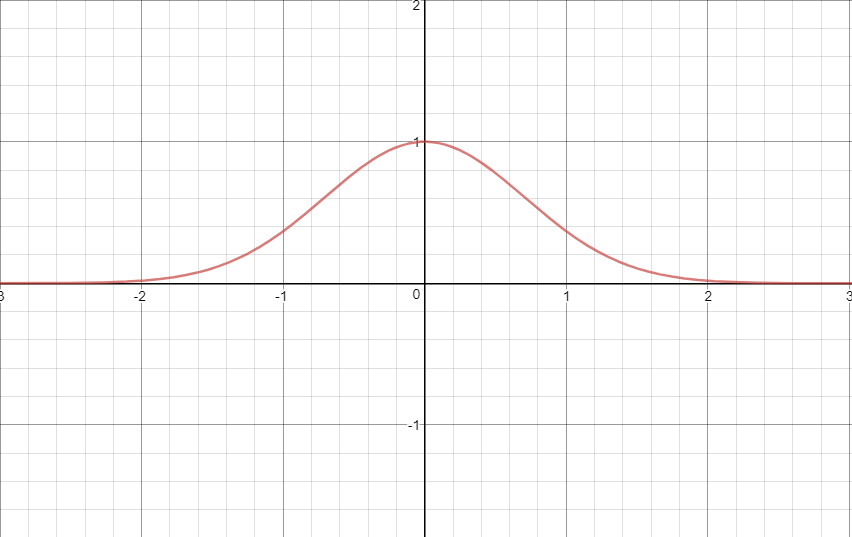
\includegraphics[width=0.3\textwidth]{1.PNG}}
  \subfloat[$f(x) = xe^{-a(x^2)}$ \\
con área de $0$]{
   \label{f:2}
    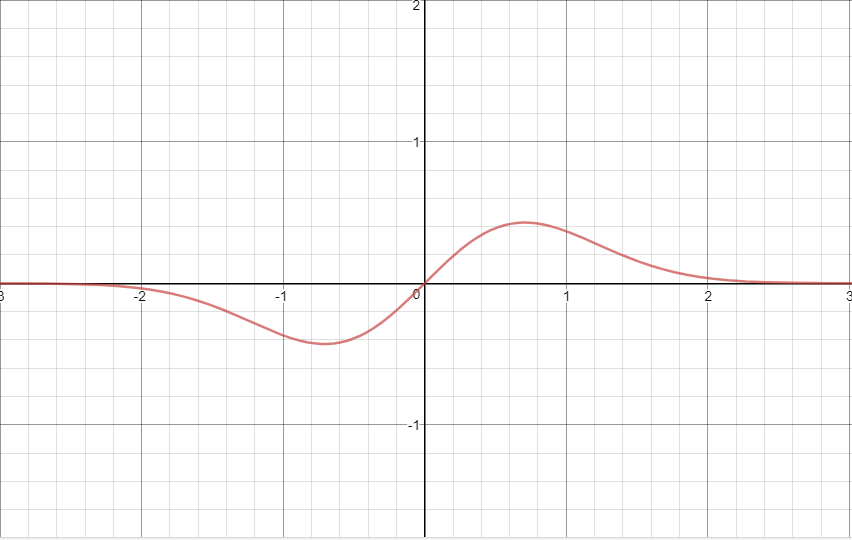
\includegraphics[width=0.3\textwidth]{2.PNG}}
  \subfloat[$f(x) = x^{2}e^{-a(x^2)}$ \\
con área de $\frac{1}{2} \sqrt{\pi \ a^{3}}$]{
   \label{f:3}
    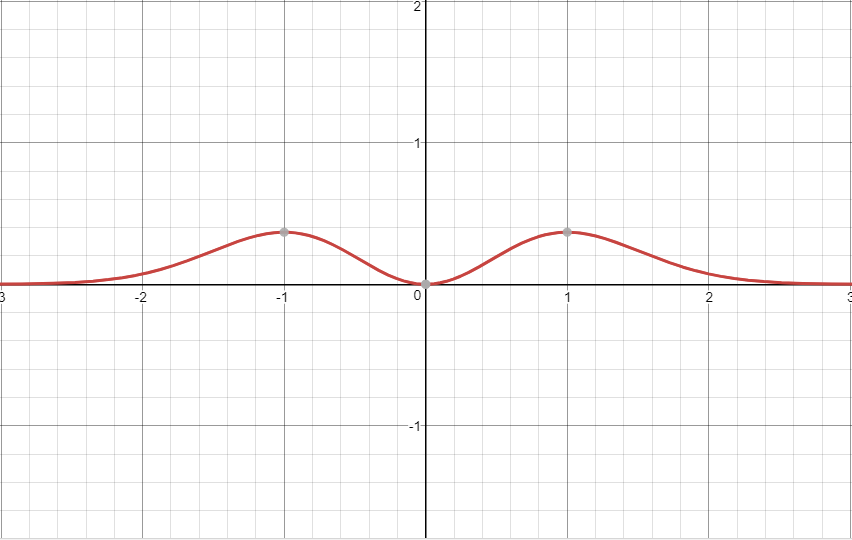
\includegraphics[width=0.3\textwidth]{3.PNG}}
 \caption{Esperanza Matemática entre V.A.}
 \label{f:Esperanza Matemática entre V.A.}
\end{figure}
\section{Covarianza y Varianza}\index{Covarianza y Varianza}
La covarianza de dos V.A. se define como: 
$$Cov (X,Y) = E(X,Y)-E(X)E(Y)$$
La varianza de $X$ se define como:
$$Var (X) = Cov (X,X)$$

Ejercicio: Si $X$ y $Y$ son V.A. integrables e independientes, demostrar que $E[XY]$ es igual $E[X]E[Y]$.
\ \\%
Si son independientes, entonces: $f(x,y)=f(x)f(y)$, por tanto
$$E(X,Y) = \int_{-\infty}^{\infty} xy f(x,y)dxdy = \int_{-\infty}^{\infty} xf(x)dx \int_{-\infty}^{\infty} yf(y)dy = E(x)E(y)$$
Ejercicio: Si $X$ y $Y$ son variables independientes, comprobar que la covarianza de $X$ y $Y$ es igual a cero.
$$Cov(X,Y) = E(XY) - E(X)E(Y),$$
Por el ejemplo anterior se sabe que $E(X,Y) = E(X)E(Y)$ y por lo tanto:
$$Cov(X,Y)= E(X)E(Y) - E(X)E(Y) = 0$$
Nota: Si la covarianza de dos variables aleatorias es igual a cero, no quiere decir que sean independientes. Sin embargo, cuando las dos variables aleatorias tienen distribución gaussiana, se cumple que $Cov(X,Y) = 0 \leftrightarrow Y$ y $X$ son independientes. 
\ \\%
Ejemplo: Calcular la varianza de una variable aleatoria $X$ que está normalmente distribuida.
$$f(x)= \frac{1}{\sqrt{2\pi D}} e^{-u^2/2}$$
$Var(X)=Cov(X,X)=E(XX)-E(X)E(X)$ donde se sabe de antemano que $E(X)=m$, por tanto:
$$Cov(X,X)= E(XX)-E(X)E(X) = \int_{-\infty}^{\infty} x^2 \frac{1}{\sqrt{2\pi D}} e^{\frac{(x-m)^2}{2D}} dx - m^2$$
Se integra mediante $u$ y $du$ donde:
\begin{itemize}
    \item $ u = \frac{x-m}{\sqrt{D}} $ 
    \item $ du = \frac{dx}{\sqrt{D}} dx$
\end{itemize}
$$ E[X^2] = \int_{-\infty}^{\infty} x^{2} f(x) dx = \frac{\sqrt{D}}{\sqrt{2 \pi D}} \int_{-\infty}^{\infty}(m+u\sqrt{D})^{2} e^{\frac{-u^{2}}{2}} du$$

$$  E[X^2] = \frac{m^{2}}{\sqrt{2 \pi}} \int_{-\infty}^{\infty} e^{\frac{-u^{2}}{2}} + \frac{2m\sqrt{D}}{\sqrt{2 \pi}} \int_{-\infty}^{\infty} e^{\frac{-u^{2}}{2}} + \frac{D}{\sqrt{2 \pi}} \int_{-\infty}^{\infty} (u^{2})e^{\frac{-u^{2}}{2}}$$
Recordando la \textbf{Figura 1.6.1}:
$$  E[X^2] = m^{2} + 0 + \frac{D}{\sqrt{2\pi}} \frac{1}{2} \frac{\sqrt{8}}{1} = m^{2} + D$$
\section{Suma de Variables Aleatorias}\index{Suma de Variables Aleatorias}
Sea $X$ y $Y$ dos V.A. independientes con función de densidad $f$ y $g$ respectivamente, si $h$ es la función de densidad $X$ y $Y$, entonces
$h(z)=\int f(x)g(z-x) dx,$ donde $Z=X+Y$.
\ \\%
Ejemplo: Si $X \sim N(0,1)$ y $Y \sim N(0,4)$, calcular la función de densidad de la suma.
$$f(x)= \frac{ e^{-u^2/2}}{\sqrt{2\pi}}$$
$$g(x)= \frac{ e^{-u^2/2}}{2\sqrt{2\pi}}$$ 
$$h(z)=\int_{-\infty}^{\infty} \frac{ e^{-u^2/2}}{\sqrt{2\pi}}\frac{ e^{-u^2/2}}{2\sqrt{2\pi}} dx = \frac{1}{4\pi}\int_{ -\infty }^{ \infty}e^{-\frac{(z-x)^2}{8}-\frac{x^2}{2}}dx = \frac{1}{4\pi}\int_{ -\infty }^{ \infty}e^{-\frac{-z^2}{8}-\frac{5}{8}x^2+\frac{2zx}{4}}dx$$ 
$$h(z)= \frac{e^{\frac{-z^2}{8}}}{4\pi}\int_{ -\infty }^{ \infty}e^{-\frac{2zx}{8}-\frac{5x^2}{8}}dx = \frac{e^{\frac{-z^2}{8}}}{4\pi}\int_{ -\infty }^{ \infty}e^{-\frac{5}{8}(\frac{2zx}{5}+x^2)}dx = \frac{e^{\frac{-z^2}{8}}}{4\pi}\int_{ -\infty }^{ \infty}e^{-\frac{5}{8}(\frac{2zx}{5}+x^2+\frac{z^2}{25}-\frac{z^2}{25})}dx$$
$$h(z)= \frac{e^{\frac{-z^2}{8}}}{4\pi}\int_{ -\infty }^{ \infty}e^{-\frac{5}{8}((x-\frac{z}{5})^2-(\frac{z}{5})^2)} dx = \frac{e^{\frac{5z^2}{200}}e^{\frac{-z^2}{8}}}{4\pi}\int_{ -\infty }^{ \infty}e^{-\frac{5}{8}((x-\frac{z}{5})^2} dx$$
Haciendo un cambio de variable $w=x-\frac{z}{5}$ y $dw=dx$ tenemos:
$$\frac{e^{\frac{5z^2}{200}}e^{\frac{-z^2}{8}}}{4\pi}\int_{ -\infty }^{ \infty}e^{-\frac{5}{8}((w)^2} dw = \frac{e^{\frac{5z^2}{200}}e^{\frac{-z^2}{8}}}{4\pi} \sqrt{\frac{\pi}{\frac{5}{8}}}=\frac{e^{\frac{-z^2}{10}}}{\sqrt{10\pi}}$$
De esta última ecuación se puede inferir que $Z \sim N(0,5)$
Nota: La función de densidad de la suma de 2 V.A. independientes con media $m_{1}$ y $m_{2}$; y varianza $D_{1}$ y $D_{2}$ respectivamente, es de nuevo una función de densidad normal: $N(m_{1}+m_{2}, D_{1}+ D_{2})$.
\section{Esperanza Condicional}\index{Esperanza Condicional}
Sean X y Y variables aleatorias, la esperanza matemática de X dado que Y toma un valor específico $y$, se define como: $$E(X|Y=y)=E(X|\mathcal{G})$$
donde $\mathcal{G}$ es un $\sigma-algebra$ contenido en un $\sigma-algebra \mathcal{F}$. El análisis se puede dividir en dos casos:
\begin{itemize}
\item Caso continuo: $$E(X|Y=y)=\int_{-\infty}^{\infty} xf(x|y) dx$$ d
Donde $f(x|y)$ se define como: $$\frac{f(x|y)}{f(y)}$$
\item Caso discreto: $$E(X|Y=y)=\sum_{x\subset R_X}xP(X=x|Y=y)$$ 
Donde $R_{x}$ es el conjunto imagen de la variable aleatoria $X$ condicionada por $Y$.
\end{itemize}
Si se compara con el $E(X)$, entonces:
$$E(x)=\sum_{x\subset R_X}xP(X=x)=\sum_{k\ge 1}x_kP(X=x_k)=\sum_{k=1}^nx_kP(X=x_k)$$
Ejercicio: Considere el experimento "lanzar dos dados", el espacio muestral, $\sigma-algebra$ y la medida de probabilidad para el experimento son: 
$$\Omega=\lbrace \omega =(i,j): i,j=1,2,3,4,5,6\rbrace$$ $$\mathcal{F}=2^{\Omega}=\sigma-algebra$$ $$P(\lbrace\Omega\rbrace)=\frac{1}{36}; \ \omega\in\Omega$$ 
Con la variable aleatoria $X$ definida como $X(\omega)= i+j$  y $Y(\omega)=\textit{min}(\textit{i,j})$. 
\begin{itemize}
\item a) Calcule el valor esperado de la variable aleatoria $X$
\[
\Omega=\left \{
    \begin{tabular}{cccccc}
    11 & 12 & 12 & 14 & 15 & 16 \\
    21 & 22 & 23 & 24 & 25 & 26 \\
    31 & 32 & 33 & 34 & 35 & 36 \\
    41 & 42 & 43 & 44 & 45 & 46 \\
    51 & 52 & 53 & 54 & 55 & 56 \\
    61 & 62 & 63 & 64 & 65 & 66 
    \end{tabular}
\right \}
\]
\ \\%
Dado que $X(\Omega)=i+j$, entonces: $$R_x=\lbrace2,3,4,5,6,7,8,9,10,11,12\rbrace$$
Por lo que, la esperanza de $X$ sería: 
$$E(x)=\sum_{k=1}^{11}x_kP(X=x_k)$$ $$E(X)=x_1P(X=x_1) + x_2P(X=x_2) + \dots + x_{11}P(X=x_{11})$$
$$E(X)=2\frac{1}{36}+3\frac{2}{36}+4\frac{3}{36}+5\frac{4}{36}+6\frac{5}{36}+\dots+11\frac{10}{36}=7$$ $$E(X)=7$$
\item b) Calcular el valor esperado de la variable aleatoria X dado que Y es igual a 3
\ \\% 
Para nuestro caso: $$E(X|Y=3)$$ 
\ \\%
Lo que quiere decir, que el mínimo de $(i,j)$ debe ser igual a tres. El conjunto de eventos que puede lograr eso sería: 
$$A=\lbrace33,34,35,36,43,53,63\rbrace$$ 
Esta clase de eventos, formalmente se describen como:
$$A_{i}=\lbrace \omega\in\Omega: Y(\omega)= y_{i} \rbrace, i=1,2,3,...$$
Entonces:
$$E(X|Y=3)=\sum_{x\in R_x|Y=3}xP(X=x|Y=y)$$
Donde
$$(R_x|Y=3)=\lbrace6,7,8,9\rbrace$$ 
\ \\%
Por lo tanto:
$$E(X|Y=3)=6\frac{1}{7}+7\frac{2}{7}+8\frac{2}{7}+9\frac{2}{7}$$ $$E(X)=\frac{54}{7}$$
\item c) Calcular el valor esperado de las siguientes condiciones para la variable aleatoria:
$$E(X|Y=1), E(X|Y=2), E(X|Y=4), E(X|Y=5), E(X|Y=6)$$ 
\ \\%
Para $E(X|Y=1)$: 
$$E(X|Y=1)=\sum_{x\in R_X|Y=1}xP(X=x|Y=1)$$ 
$$A_{y}=\lbrace 11,12,13,14,15,16,21,31,41,51,61\rbrace$$ $$|A_{y}|=11$$ $$(R_X|Y=1)=\lbrace 2,3,4,5,6,7\rbrace$$ $$E(X|Y=1)=2\frac{1}{11}+3\frac{2}{11}+4\frac{2}{11}+5\frac{2}{11}+6\frac{2}{11}+7\frac{2}{11}$$
$$E(X|Y=1)=\frac{52}{11}$$
Para $E(X|Y=2)$: 
$$E(X|Y=2)=\sum_{x\in R_x|Y=2}xP(X=x|Y=2)$$ $$A_y=\lbrace 23,24,25,26,22,32,42,52,62\rbrace$$ $$|A_y|=9$$ $$(R_X|Y=2)=\lbrace 4,5,6,7,8\rbrace$$ $$E(X|Y=2)=4\frac{1}{9}+5\frac{2}{9}+6\frac{2}{9}+7\frac{2}{9}+8\frac{2}{9}$$ $$E(X|Y=2)=6$$
Para $E(X|Y=4)$: 
$$E(X|Y=4)=\sum_{x\in R_x|Y=4}xP(X=x|Y=4)$$ $$A_y=\lbrace 44,45,46,54,64\rbrace$$ $$|A_y|=5$$ $$(R_X|Y=4)=\lbrace 8,9,10\rbrace$$ $$E(X|Y=4)=8\frac{1}{5}+9\frac{2}{5}+10\frac{2}{5}=\frac{46}{5}$$
Para $E(X|Y=5)$: 
$$E(X|Y=5)=\sum_{x\in R_x|Y=5}xP(X=x|Y=5)$$ 
Entonces:
$$E(E(X|Y=y_i))=\sum_{y=R_x}E(X|Y)P(Y=y_i)$$
Donde 
$$R_Y=\lbrace 1,2,3,4,5,6\rbrace=\lbrace y_1,y_2,y_3,y_4,y_5,y_6\rbrace$$ 
Como se hablan de todas las variables, se puede generalizar: 
$$E(E(X|Y=y_i))=E(E(X|Y))$$ 
Al trabajarlo, se observa que: 
$$E(E(X|Y))=E(X)$$ 
El resultado obtenido, no es sólo para el caso del experimento de "lanzar dos dados", el resultado es una identidad y pasa para toda variable independiente $X$ y $Y$. 
\end{itemize}
\section{Convergencia de Variables Aleatorias}\index{Convergencia de Variables Aleatorias}
Sean $X$ y $X_n, n=1,2,...$ V.A. defenidas en $(\Omega ,f,P)$; la convergencia de la sucesión $(X_n)n\geq 1$, hacia $\overline{X}$ se puede definir de varias formas, dependiendo de como se mida la diferencia entre $X_{n}$ y $X$
\ \\%
Límite se la secuencia:
\begin{itemize}
    \item Sentido casi seguro: $P( w: \lim_{n \to \infty} X_{n}(w) = X(w)) = 1$
    \item En probabilidad: $ \lim_{n \to \infty} P(w:| X_{n}(w)-X_{n}|\leq \epsilon) = 1 $
    \item Distribución: $ \lim_{n \to \infty} E[X_{n}] = E[X] $
    \item Promedio cuadrático: $ \lim_{n \to \infty} E[(X_{n}-X)^2] = 0$
\end{itemize}
Sea $(X_n)n\geq 1$ una sucesión tal que las V.A. de la sucesión tienen valor esperado $\mu$, la misma varianza $\alpha ^{2}$ con varianza $0$ entre ellos. El término genérico de la sucesión es:
$$\bar{X_n}=\frac{1}{n}\sum_{n}^{1}X_i$$
Evaluar $\lim_{n\rightarrow \infty }E[(\bar{X_n}-X)]$ siendo $\mu=X$:

$$\lim_{n\rightarrow \infty }E[({X_n}-\mu)^2] = E[{X_n}] = E[ \frac{1}{n}\sum_{1}^{n}X_i] = \frac{1}{n}E[ \sum_{1}^{n}X_{i}] =\frac{1}{n}\sum_{n}^{1}E(X_i) = \frac{1}{n}(n\mu)=\mu $$
$$Var(\bar{X_n})=E\left \lfloor (\bar{X_n}-E(\bar{X_n})^2 \right \rfloor =Var(\frac{1}{n}\sum_{1}^{n}X_i)$$
$$Var(aX)=a^2Var(X) =\frac{1}{n^2}Var(\sum_{1}^{n}X_i) $$
$$ \frac{1}{n^2}\sum_{1}^{n}Var(X_i) =\frac{1}{n^2}\sum_{1}^{n}\Theta ^2 =\frac{\Theta ^2}{n}$$
$$\therefore \lim E\left [ (\bar{X_n}-\mu )^2 \right ]=\lim_{n\rightarrow \infty }\frac{\Theta ^2}{n}=0$$

\textbf{Proposición 2.14.1}(Ejercicio)
\ \\%
Sea $X_{n}$ una sucesión de una V.A. tal que hay una constante $k$ con $E\left \lfloor X_{n} \right \rfloor\rightarrow k $ y $Var\left \lfloor X_{n} \right \rfloor\rightarrow 0$, cuando $ n \rightarrow \infty\ $  demuestra que $ ms-\lim_{n \to \infty }=k$:
$$\lim_{n \to \infty }E\left \lfloor (X_n-X)^2 \right \rfloor=0$$
$$X=k$$
$$\lim_{n \to \infty } E\left \lfloor (X_n-X)^2 \right \rfloor$$
$$\lim_{n \to \infty }E(X_n)=k$$
$$\lim_{n\rightarrow \infty }\left \lfloor E(X_n^2)-E(X_n)^2 \right \rfloor=0$$
$$\lim_{n \to \infty }\left \lfloor E(X_n^2)-2E(X_n)E(X)+E(X^2) \right \rfloor$$
$$\lim_{n \to \infty }\left \lfloor E\left \lfloor X_n^2 \right \rfloor-2kE(X_n)+k^2 \right \rfloor$$
$$\lim_{n \to \infty }\left \lfloor E(X_n^2)-E(X_n)^2+E(X_n)^2-2kE(X_n)+k^2 \right \rfloor$$
$$\lim_{n \to \infty }\left \lfloor E(X_n^2)-E(X_n)^2 \right \rfloor+\lim_{n \to \infty }\left \lfloor E(X_n)^2+2kE(X_n)+k^2 \right \rfloor$$
$$\lim_{n \to \infty }\left \lfloor (E(X_n)-k)^2 \right \rfloor$$
$$(\lim_{n \to \infty }E(X_n)-k)^2=(k-k)^2=0$$
\ \\%
Desigualdad de Jensen
$$\varnothing (E(X))\leq E(\varnothing (X)))$$
$$(E(X_n)-E(X))^2$$
$$(E\left \lfloor X_n-X \right \rfloor)^2$$
$$0\leq E(X_n-X)^2\leq E\left \lfloor (X_n-X)^2 \right \rfloor=0$$
Entonces:
$$ E(X_n-X)^2 = 0 $$ 
\newpage
\section{Tareas}
\subsubsection{Tarea 1}
Ejercicio: Proponer 3 experimentos aleatorios y 3 no aleatorios.
\begin{itemize}
    \item Aleatorios
    \begin{itemize}
        \item Juego de ruleta (casino)
        \item Lanzar un dado
        \item Lanzar una moneda
    \end{itemize}
    \item No Aleatorios
    \begin{itemize}
        \item Meter la mano al fuego
        \item Tirar una pelota de un edificio
        \item Combinar amarillo con azul y obtener verde
    \end{itemize}
\end{itemize}
Ejercicio: Lance una moneda tres veces y observe la secuencia de caras (c) y sellos (s). Establezca el espacio muestral del experimento aleatorio.
$$ \Omega = \left\{ ccc,ccs,csc,css,ssss,ssc,scs,scc\right\} $$
Ejercicio: Considere el experimento aleatorio "Lanzar una moneda y un dado".
\begin{itemize}
    \item ¿Cúal es el espacio muestral del experimento?
    $$ \Omega = \left\{ c1,c2,c3,c4,c5,c6,s1,s2,s3,s4,s5,s6 \right\} $$
    \item Exprese explícitamente el evento $A_{1} = $ aparece cara y un número par.
    $$ A_{1} = \left\{ c2,c4,c6 \right\} $$
    \item Exprese explícitamente el evento $A_{2} = $ aparece un número menor que tres.
    $$ A_{2} = \left\{ c1,c2,s1,s2 \right\} $$
    \item Exprese explícitamente el evento $A_{3} = $ aparece sello y un número impar.
    $$ A_{3} = \left\{ s1,s3,s5 \right\} $$
\end{itemize}
Ejercicio: Considere el experimento "Lanzar una modena". Se observa que el espacio muestral es  $ \Omega = \left\{ c,s \right\}$.
\begin{itemize}
    \item Verifique que $\left\{ I, \Omega \right\}$ es un $\sigma-algebra$
    \begin{enumerate}
    \item $z$ no esta vacía, contiene al menos un elemento
    \item $A_{1} = I \rightarrow A^{c} = \Omega$ y  $\Omega \in z$ y 
    $A_{2} = \Omega \rightarrow A^{c} = I$ y  $I \in z$
    \item $A_{1} \bigcup A_{2} = I \bigcup \Omega = \Omega \therefore \Omega \in z$
    \item $A_{1} \bigcap A_{2} = I \bigcup I = I \therefore I \in z$
\end{enumerate}
    \item Verifique que $\left\{ I,c,s, \Omega \right\}$ es un $\sigma-algebra$
    \begin{enumerate}
    \item $z$ no esta vacía, contiene al menos un elemento
    \item $A_{1} = I \rightarrow A^{c} = \Omega$ y  $\Omega \in z$ y 
    $A_{2} = \Omega \rightarrow A^{c} = I$ y  $I \in z$\\
    $A_{3} = c \rightarrow A^{c} = s$ y  $s \in z$ y 
    $A_{4} = s \rightarrow A^{c} = c$ y  $c \in z$
    \item $A_{1} \bigcup A_{2} \bigcup A_{3} \bigcup A_{4} = I \bigcup c \bigcup s \bigcup \Omega = \Omega \therefore \Omega \in z$
    \item $A_{1} \bigcap A_{2} \bigcap A_{3} \bigcap A_{4} = I \bigcap c \bigcap s \bigcap \Omega = I \therefore I \in z$
\end{enumerate}
    \item Proponga un conjunto que no sea un $\sigma-algebra$ y explique: $$ z =  \left\{ I,c,s,1, \Omega \right\} $$
    \begin{enumerate}
    \item $z$ no esta vacía, contiene al menos un elemento
    \item $A_{1} = I \rightarrow A^{c} = \Omega$ y  $\Omega \in z$ y 
    $A_{2} = c \rightarrow A^{c} = \left\{ I,s,1, \Omega \right\}$ y  $\left\{ I,s,1, \Omega \right\} \notin z$
\end{enumerate}
\end{itemize}
Ejercicio: Escriba cada uno de los posibles eventos del siguiente espacio muestral $\Omega = \left\{ a,b,c,d \right\} $.
$$ F = 2^{\Omega} = \left\{ I,a,b,c,d, \left\{ a,b \right\}, \left\{ a,c \right\}, \left\{ a,d \right\}, \left\{ b,c \right\}, \left\{ b,d \right\}, \left\{ c,d \right\}, \left\{ a,b,c \right\}, \right\}  $$ 
$$ \left\{ \left\{ a,b,d \right\}, \left\{ b,c,d \right\}, \left\{ a,c,d \right\}, \Omega  \right\}     $$
Ejercicio: Se lanza un dado. Considere que $A = \left\{ 2,4,6 \right\}$, $B = \left\{ 1,3,5 \right\}$ y que $C = \left\{ 1,2,3,5  \right\}$. Demostrar que $\left\{ I,A,B, \Omega \right\}$ es un $\sigma-algebra$ y que $\left\{ I,A, \Omega \right\}$ y $\left\{ I,A,B,C \Omega \right\}$ no son $\sigma-algebra$.
\begin{itemize}
    \item Para: $\left\{ I,A,B, \Omega \right\}$
    \begin{enumerate}
        \item $z$ no esta vacía, contiene al menos un elemento
        \item $A_{1} = I \rightarrow A^{c} = \Omega$ y  $\Omega \in z$ y 
        $A_{2} = \Omega \rightarrow A^{c} = I$ y  $I \in z$\\
        $A_{3} = A \rightarrow A^{c} = B$ y  $B \in z$ y 
        $A_{4} = B \rightarrow A^{c} = A$ y  $A \in z$
        \item $A_{1} \bigcup A_{2} \bigcup A_{3} \bigcup A_{4} = I \bigcup c \bigcup s \bigcup \Omega = \Omega \therefore \Omega \in z$
        \item $A_{1} \bigcap A_{2} \bigcap A_{3} \bigcap A_{4} = I \bigcap c \bigcap s \bigcap \Omega = I \therefore I \in z$
    \end{enumerate}
    \item Para: $\left\{ I,A, \Omega \right\}$
    \begin{enumerate}
        \item $z$ no esta vacía, contiene al menos un elemento
        \item $A_{1} = I \rightarrow A^{c} = \Omega$ y  $\Omega \in z$ y 
        $A_{2} = \Omega \rightarrow A^{c} = I$ y  $I \in z$\\
        $A_{3} = A \rightarrow A^{c} = B$ y  $B \notin z$
    \end{enumerate}    
    \item Para: $\left\{ I,A,B,C \Omega \right\}$
    \begin{enumerate}
        \item $z$ no esta vacía, contiene al menos un elemento
        \item $A_{1} = I \rightarrow A^{c} = \Omega$ y  $\Omega \in z$ y 
        $A_{2} = \Omega \rightarrow A^{c} = I$ y  $I \in z$\\
        $A_{3} = C \rightarrow A^{c} =\left\{ 4,6 \right\} $ y  $ \left\{ 4,6 \right\} \notin z$ 
    \end{enumerate}    
\end{itemize}
\subsubsection{Tarea 2}
Ejercicio: Se lanza una moneda al aire hasta que aparezca cara. Sea $X(w)$ el número de veces que se lanza la moneda, determine el espacio muestral del experimento aleatorio y el conjunto imagen de la variable aleatoria discreta.
$$ \Omega = \left\{ c,s \Omega \right\} $$
$$ R(x) = \left\{ 1,2,3,4,5,..... \Omega \right\} $$
Ejercicio: Un lote de 500 piezas contiene 10 piezas que no cumplen con los requerimientos del cliente. Se seleccionan piezas sucesivamente sin remplazo, hasta que se obtiene la primera pieza que no cumple. Determine el conjunto imagen de la variable aleatoria, si $x(w)$ es el número de piezas seleccionadas.
$$ R(x) = \left\{ 1,2,3,4,5,.....,491 \right\} $$
Ejercicio: Verificar los axiomas de Kolmogorov para el lanzamiento de un dado considerando el $\sigma-algebra $ $F$ como $\left\{ I,\left\{ 1,3,5  \right\}, \left\{ 2,4,6  \right\}, \Omega  \right\} $
\begin{itemize}
    \item Axioma 1: $A_{1} = I$, $A_{2} = \left\{ 1,3,5  \right\}$, $A_{3} = \left\{ 2,4,6  \right\}$ y $A_{4} = \Omega \therefore$\\ 
    $P(A_{1}) = 0/2, 0 $, $P(A_{2}) = 1/2 , .5 > 0$, $P(A_{3}) = 1/2, 0 > 0$ y $P(A_{4}) = 2/2, 1 > 0$
    \item Axioma 2: $P(A_{4}) = 2/2= 1 = P(\Omega)$
    \item Axioma 3:
    \begin{itemize}
        \item $A_{1}$ y $A_{2}$: $P(A_{1} \cup A_{2}) = .5$ y $P(A_{1}) + P(A_{2}) = .5$
        \item $A_{1}$ y $A_{3}$: $P(A_{1} \cup A_{3}) = .5$ y $P(A_{1}) + P(A_{3}) = .5$
        \item $A_{1}$ y $A_{4}$: $P(A_{1} \cup A_{4}) = 1$ y $P(A_{1}) + P(A_{4}) = 1$
        \item $A_{2}$ y $A_{3}$: $P(A_{2} \cup A_{3}) = 1$ y $P(A_{2}) + P(A_{3}) = 1$
    \end{itemize}
\end{itemize}
Ejercicio: Usando los axiomas de Kolmogorov, comprobar los siguientes teoremas de probabilidad.
\begin{itemize}
    \item $P(I) = 0 \therefore A \cup I = A; A \cap I = I \therefore P(A) = P(A \cup I) = P(A) + P(I) \therefore P(A) = P(A) + P(I) \therefore P(A) - P(A) = P(I) = 0$
    \item $P(A^{c})= 1 - P(A) \therefore P(\Omega) = 1; P(\Omega) = P(A^{c} \cup A) = 1 \therefore P(\Omega) = P(A^{c}) + P(A) = 1  \therefore P(A^{c})  = 1 - P(A)$
    \item $0 \leq P(A) \leq 1 \therefore P(A) \geq 0; P(\Omega) = 1 \therefore P(I) \leq P(A) \leq P(\Omega) \therefore 0 \leq P(A) \leq 1$
    \item Si $A c B$ entonces $P(A) \leq P(B) \therefore B = A \cup (A\arrowvert B) \therefore P(B) = P(A) + P(A\arrowvert B) \therefore si P(A\arrowvert B) \geq 0 \therefore P(A) \leq P(B)$
    \item Para 2 eventos cualquiera $A$ y $B$, se tiene que $P(A\arrowvert B) = P(A) - P(A \cap B) \therefore A = (A\arrowvert B) cup (A \cap B) \therefore P(A) = P(A\arrowvert B) + P(A \cap B) \therefore P(A\arrowvert B) = P(A) - P(A \cap B) $
    \item Para 2 eventos cualquiera $A$ y $B$, se tiene que $P(A\cup B) = P(A) + P(B) - P(A \cap B) \therefore A \cup B = (A\arrowvert B) \cup B \therefore P(A \cup B) = P(A\arrowvert B) + P(B) \therefore P(A \cup B) = P(A) - P(A \cap B) + P(B) \therefore P(A\cup B) = P(A) + P(B) - P(A \cap B)$
\end{itemize}
\subsubsection{Tarea 3}
Ejercicio: Para el experimento aleatorio "Lanzar dos dados equilibrados", considerar la variable aleatoria $X(w)$ como el valor máximo de las caras superiores de los dados. Escriba el espacio de probabilidad del experimento, además represente la función de densidad de probabilidad y la función de distribución $X(w)$ (Tablas, gráficas y utilizar la función Heaviside y Delta de Dirac).
$$ \Omega = \left\{11,12,13,14,15,16,21,22,23,24,25,26 \right\} $$
$$ \left\{31,32,33,34,35,36,41,42,43,44,45,46 \right\} $$
$$ \left\{51,52,53,54,55,56,61,62,63,64,65,66 \right\} $$
\ \\%
\textbf{Tabla}
\begin{center}
\begin{tabular}{ |c|c|c|c|c|c|c|c|c| } 
 \hline
 \(x_i\) & 1 & 2 & 3 & 4 & 5 & 6  \\ 
 \hline
 \(f(x_i)\) & \( \frac{1}{36} \) & \( \frac{3}{36} \) & \( \frac{5}{36} \) & \( \frac{7}{36} \)& \( \frac{9}{36} \) & \( \frac{11}{36} \) \\ 
 \hline
\end{tabular}
\end{center}
\textbf{Tabla}
\begin{center}
\begin{tabular}{ |c|c|c|c|c|c|c|c|c| } 
 \hline
 \(x_i\) & 1 & 2 & 3 & 4 & 5 & 6  \\ 
 \hline
 \(F(x_i)\) & \( \frac{1}{36} \) & \( \frac{4}{36} \) & \( \frac{9}{36} \) & \( \frac{16}{36} \)& \( \frac{25}{36} \) & \( \frac{36}{36} \) \\ 
 \hline
\end{tabular}
\end{center}
$$F(x) =  \frac{1}{36}  u [ 1(x - 1) + 4(x - 2) + 9(x - 3) + 16(x - 4) + 25(x - 5) + 36(x - 6) ]$$
$$f(x_i) = \frac{1}{36}  \delta [ 3(x - 1) + 5(x - 2) + 7(x - 3) + 9(x - 4) + 11(x - 5) + (x - 6)]$$
Ejercicio: Una variable aleatoria se llama de Rayleigh si su función de probabilidad está dada por:
$$f(x)= \left\{ \begin{array}{lcc}
             \frac{\alpha}{\sigma^{2}} e^{\frac{-x^{2}}{2\sigma^{2}}} &   si  &  x > 0 \\
             \\ 0 &  si & x < 0 \\
               \end{array}
   \right.$$
Determinar la función de distribución de x:
$$ \int_{0}^{x} \frac{y}{\sigma^{2}} e^{\frac{y^{2}}{2\sigma^{2}}} dy = (-e^{\frac{x^{2}}{2\sigma^{2}}}) - (-e^{\frac{0^{2}}{2\sigma^{2}}}) = 1 - e^{\frac{x^{2}}{2\sigma^{2}}} $$
Ejercicio: Sea $\alpha,\beta \in R$ demostrar que si $X$ está normalmente distribuida $X \sim N(\mu,\sigma^{2})$, entonces $Y = \alpha x + \beta$ también está normalmente distribuida con $Y \sim N(\alpha\mu + \beta,\alpha\sigma^{2})$
$$ X \sim N(\mu,\sigma^{2}) \therefore f(x) = \frac{1}{\sqrt{2 \pi \sigma}} e^{- \frac{(x - \mu)^{2}}{2 \sigma^{2}}} $$
$$ F(Y) = P(X \leq \frac{y-\beta}{\alpha}) = \int_{-\infty}^{\frac{y-\beta}{\alpha} = h} f(x) dx = \int_{-\infty}^{h} \frac{1}{\sqrt{2 \pi \sigma}} e^{- \frac{(x - \mu)^{2}}{2 \sigma^{2}}} dx $$
Se hace un cambio de variable:$z = \alpha x + \beta$ y $dz = \alpha dx$, finalmente resulta:
$$ \frac{1}{\sqrt{2 \pi \sigma^{2} \alpha^{2}}} \int_{-\infty}^{y}  e^{- \frac{z-(\alpha\mu + \beta)^{2}}{2 \sigma^{2} \alpha^{2}}} dx     $$
$$Y \sim N(\alpha\mu + \beta,\alpha\sigma^{2})$$
Ejercicio: Considere dos variables aleatorias $X$ y $Y$ independientes cuyas funciones de distribución son $f(t) = g(t) =  \lambda e^{-\lambda t} $ para $t \geq 0$ respectivamente. Calula la función de distribución $X + Y$.
$$ h(z) = \int_{0}^{z} f(x)g(z-x) dx = \int_{0}^{z} \lambda e^{-\lambda x}\lambda e^{-\lambda (z-x)} dx $$
$$ h(z) = \lambda^{2} \int_{0}^{z}  e^{-\lambda x}e^{-\lambda (z-x)}dx = \lambda^{2} e^{-\lambda z} \int_{0}^{z}  dx  $$
$$ h(z) = \lambda^{2} e^{-\lambda z} z  $$
Ejercicio: Comprobar que $\frac{1}{4\pi} \int_{-\infty}^{\infty} e^{-\frac{x^{2}}{2} - \frac{(z-x)^{2}}{8}} dx = \frac{e^{-\frac{z^{2}}{10}}}{\sqrt{10\pi}}$
$$ \frac{1}{4\pi} \int_{-\infty}^{\infty} e^{-\frac{x^{2}}{2} - \frac{(z-x)^{2}}{8}} dx =  \frac{1}{4\pi} e^{\frac{-z^{2}}{8}} \int_{-\infty}^{\infty} e^{-\frac{1}{2}\frac{5x^{2}-2xz}{4}} dx$$
$$ \frac{1}{4\pi} e^{\frac{-z^{2}}{10}} \int_{-\infty}^{\infty} e^{-\frac{1}{2}[\sqrt{3/4}x - \sqrt{5}/5\sqrt{4} z]} dx$$
$$ u = (\frac{\sqrt{5}}{\sqrt{4}} (x - z/5)); du = \frac{\sqrt{5}}{\sqrt{4}} dx $$
$$\frac{e^{-\frac{z^{2}}{10}}}{\sqrt{10\pi}}$$
Ejercicio: Demostrar que la $Cov(X,Y) = E[(X - \mu_{x})(Y - \mu_{y})]$, dodne $\mu_{x} = E[X] $ y $\mu_{y} = E[Y] $
$$ Cov(X,Y) = E[(X - \mu_{x})(Y - \mu_{y})] = E[XX] -E[X]E[Y] = E[(X - E[X])(Y - E[Y])]          $$
$$ Cov(X,Y) = E[XY - XE[Y] - YE[X] + E[X]E[Y]] = E[XY] - E[X]E[Y] $$
Ejercicio: Demostrar que $Var[x] = E[(X-\mu_{x})^{2}] \therefore$
$$ Var[x] = Cov[XX] = E[XX] - E[X]E[X] = E[x^{2} - 2x\mu_{x} - \mu_{x}^{2}] = [(X-\mu_{x})^{2}]        $$
\subsubsection{Tarea 4}
Ejercicio 2.12.8 de Ovidiu: Se lanza 4 veces una moneda equilibrada. Cada lanzamiento da como resultado cara (c) o sello (s).
\begin{itemize}
    \item ¿Cuantos elementos tiene $\Omega$ ? $2^{\Omega} = 16 $
    \item Considera los eventos A: 2 de los 4 lanzamientos son cara, B: el primer lanzamiento es sello, y C: tres de los 4 lanzamientos son cara. Calcule $P(A), P(B)$ y $P(C)$. $P= 3/8, P(B) = 1/2$ y $P(C) = 1/4$
    \item Calcule $P(A \cap B) y P(B \cap C) $: $P(A \cap B)= 3/16 y P(B \cap C) = 3/16 $
    \item ¿Los eventos A y B son indepedientes? Si
    $$ P(A \cap B) = P(A)P(B) \rightarrow 3/16 = 3/16 $$
    \item ¿Los eventos B y C son indepedientes? No
    $$ P(C \cap B) = P(C)P(B) \rightarrow 3/16 = 1/8 $$
    \item Considere los siguientes $\sigma-algebras$: $F$ se conocen lo resultados de los primeros 2 lanzamientos, $G$ se conocen los resultados de los lanzamientos pero no el orden. ¿Cómo podría expresarse en palabras el conjunto $F \cap G$?\\
    Se conocen los resultados de los primeros 2 lanzamientos, pero no el orden de los últimos 2.
    \item Pruebe que $A \in G$, $B \in F$ y $c \in G$: Son verdaderos en base a la descripsión de $A,B$ y $C$.
    \item Defina las variables aleatorias $x$: número de caras - número de sellos y  $y$: número de sellos antes de la primera cara. Muestre que $x$ es $G-medible$, mientras que $y$ no lo es.
    $$ x = C - S = \left\{ 4,2,0,-2,-4 \right\}$$ 
    $$ y = \left\{ 0,1,2,3,4,5,6,...... \right\}$$
    $Y$ no es medible porque no se conoce el orden de los resultados de los lanzamientos, por lo que no es $G-medible$. $x$ es $G-medible$, dado que se conocen los valores del resultado y se puede colocar un número en ese rango.
    \item Encuentre $E[x], E;[y] $ y $E[X \arrowvert G]$\\
    $E[x] = 0, E;[y]= 15/16 $ y $E[X \arrowvert G] = x$, dado que no es $G-medible$
\end{itemize}
Ejercicio: Sean $X$ y $Y$ variables aleatorias sobre $(\Omega, F, P)$ con función de densidad conjunta: 
$$ f(x,y) = \frac{\sqrt{3}}{4 \pi} e^{\frac{-(x^{2}-2xy +y^{2})}{2}}; x,y \in R     $$
La densidad marginal de $y$ es una función de densidad normal con media cero y varainza $\frac{4}{3}$. Calcule la función de densidad condicional $f(x \arrowvert y)$  para toda $x,y \in R$ y también la esperanza condicional $C[X \arrowvert Y = y]$.
$$ F(x \arrowvert y) = \frac{f(x,y)}{f(y)} \therefore$$
$$ F(x \arrowvert y) = \frac{\frac{\sqrt{3}}{4 \pi} e^{\frac{-(x^{2}-2xy +y^{2})}{2}}}{\frac{1}{\sqrt{2 \pi \frac{4}{3}}} e^{\frac{-y^{2}}{2(4/3)}}} = \frac{1}{\sqrt{2 \pi}} e^{{\frac{-1}{2}} (x - (y/2))^{2}} $$
$$ \int_{-\infty}^{\infty} x f(x \arrowvert y) dx = \frac{x}{\sqrt{2 \pi}} e^{{\frac{-1}{2}} (x - (y/2))^{2}} $$
$$ u = x- \frac{y}{2}, du = dx \therefore   $$
$$ \int_{-\infty}^{\infty} x f(x \arrowvert y) dx = \int_{-\infty}^{\infty} \frac{x}{\sqrt{2 \pi}} e^{{\frac{-1}{2}} (x - (y/2))^{2}}  dx $$
$$ \int_{-\infty}^{\infty} (u - \frac{y}{2}) \frac{1}{\sqrt{2 \pi}} e^{{\frac{-1}{2}} u^{2}}  dx  = 0 + \frac{y}{2} = \frac{y}{2} $$
\ \\%
Ejercicio: Una persona está atrapada en una mina que tiene tres caminos. El primer camino conduce a la salida después de un trayecto de 3 horas, el segundo y tercer camino llevan a la persona al punto de partida después de 5 y 7 horas respectivamente. Sea $X$ el tiempo requerido para salir de la mina y $X$ el camino elegido por la persona la primera vez. Determine:
\begin{itemize}
    \item El conjunto imagen de $X$: $ R_{X} = \left\{ 3,8,10,15 \right\}  $
    \item El conjunto imagen de $Y$: $ R_{Y} = \left\{ 1,2,3 \right\} $
    \item Espacio muestral de $X$: $ \Omega = \left\{ 1, \left\{ 2,1 \right\}, \left\{ 3,1 \right\}, \left\{ 2,3,1 \right\}, \left\{ 3,2,1 \right\} \right\} $
    \item $E[X \arrowvert Y=1 ] = 3(1) = 3 $
    \item $E[X \arrowvert Y=3 ] = 12.5      $
    \item $P(Y=1) = 1/3 $
    \item $E[E[X \arrowvert Y]] = 3(1/3) + 23/2 (1/3) + 25/2 (1/3) = 9$
    \item $E[X] = 3\frac{1}{3} + 8\frac{1}{3}\frac{1}{2} + 10\frac{1}{3}\frac{1}{2}  + 15\frac{1}{3}\frac{1}{2}(1) + 15\frac{1}{3}\frac{1}{2}(1) = 9 $
\end{itemize}
\newpage
\subsubsection{Tarea 5}
Ejercicio: Si $X_{n}$ tiende a $X$ en promedio cuadrático, demostrar que $E[X_{n} \arrowvert H]$ tiende a $E[X_{n} \arrowvert H]$ tiende a $E[X \arrowvert H]$ en promedio cuadrático.
$$ms-X_{n} \to X \therefore ms-E[X_{n} \arrowvert H] \to E[X \arrowvert H] $$
$$ \lim_{n \to \infty} E[(E[X_{n} \arrowvert H] - E[X \arrowvert H] )^{2}] $$
$$ \lim_{n \to \infty} E[(E[X_{n} - X \arrowvert H] )^{2}] \leq \lim_{n \to \infty} E[(E[(X_{n} - X)^{2} \arrowvert H] ] = 0    $$
Ejercicio: Si $ms- \lim_{n \to \infty} X_{n} = 0$ y $ms- \lim_{n \to \infty} Y_{n} = 0$, demostrar que: $ms- \lim_{n \to \infty} X_{n} - Y_{n} = 0$
$$ \lim_{n \to \infty} E[(X_{n} + Y_{n})^{2}]  = \lim_{n \to \infty} E[X_{n}^{2} + 2X_{n}Y_{n} + Y_{n}^{2} ] $$
$$ \lim_{n \to \infty} E[2X_{n}Y_{n}]  = 2\lim_{n \to \infty} E[X_{n}]E[Y_{n}] = 2(0) = 0$$
Ejercicio: Si las sucesiones de variables aleatorias $X_{n}$ y $Y_{n}$ convergen en promedio cuadrático, demuestre que:
\begin{itemize}
    \item $ms- \lim_{n \to \infty} (X_{n} + Y_{n}) = ms- \lim_{n \to \infty} X_{n} + ms- \lim_{n \to \infty} Y_{n} $
    Se sabe que:
    $$ ms- \lim_{n \to \infty} X_{n} = 0     $$
    $$ ms- \lim_{n \to \infty} Y_{n} = 0     $$
    $$ \lim_{n \to \infty} E[X_{n}^{2}] = 0  $$
    $$ \lim_{n \to \infty} E[X_{n}^{2}] = 0  $$
    $$ \lim_{n \to \infty} X_{n} + Y_{n} = 0 $$
    $$ \lim_{n \to \infty} E[(X_{n} + Y_{n})^{2}] = 0  \therefore $$
    Por tanto:
    $$ \lim_{n \to \infty} E[(X_{n} + Y_{n})^{2}]  = \lim_{n \to \infty} E[X_{n}^{2} + 2X_{n}Y_{n} + Y_{n}^{2} - 2X_{n}Y_{n} $$
    $$ ms- \lim_{n \to \infty} X_{n} + ms- \lim_{n \to \infty} Y_{n} $$
    \item $ms- \lim_{n \to \infty} c X_{n} = c ms- \lim_{n \to \infty} X_{n}$, donde $c \in R$
    $$ \lim_{n \to \infty} E[(cX_{n})^{2}] = \lim_{n \to \infty} E[c^{2}X_{n}^{2}]       $$
    $$ \lim_{n \to \infty} E[c^2] E[X_{n}^{2}] = 0      $$
    $$ c \lim_{n \to \infty} E[X_{n}^{2}] = c \lim_{n \to \infty}[0] = c[0] = 0      $$
\end{itemize}
%-----------------------------------------------------------------------
%	CHAPTER 2
%-----------------------------------------------------------------------
\chapter{Segundo Parcial: Porcesos Estocásticos}
\section{Procesos Estocásticos}\index{Procesos Estocásticos}
Un proceso estocástico es una familia de V.A. definidas en un espacio de probabilidad $(\Omega,F,P)$.
\ \\%
Los procesos estocásticos tienen realixaciones, es decir cada una de las trayectorias obtenidas.
\ \\%
Ejemplo: En el experimento lanzar una moneda se define el proceso estocástico como:
$$X(\omega, t)= \left\{ \begin{array}{lcc}
             sen(t) &   si  & \omega = \text{cara} \\
             \\ 2t &  si & \omega = \text{sello} \\
               \end{array}
   \right.$$
\section{Movimiento Browniano}\index{Movimiento Browniano}
Si $X_{t}=-B_{r}$\:entonces\:$X_{t}$ es un movimiento browniano.
\ \\%
Nota: $X_{r}=-B_{r}$ y $X_{s}=-B_{s}$
\begin{itemize}
    \item Condición 1: En $t=0, X_{0}=-B_{0}=-0=0$  
    \item Condición 2: $Cov(X_{s}-X_{r},X_{r}-X_{0})=0$ es decir, independientes para $0 \leq r \leq s $
    $$Cov(X_{s}-X_{r},X_{r}-X_{0})=E[X_{s}-X_{r},X_{r}-X_{0}]-E[X_{s}-X_{r}]E[X_{r}-X_{0}]$$
    $$Cov(X_{s}-X_{r},X_{r}-X_{0})=E[X_{s}X_{r}-X_{r}^2]-E[X_{s}-X_{r}]E[X_{r}]$$
    $$Cov(X_{s}-X_{r},X_{r}-X_{0})=E[X_{s}X_{r}]-E[X_{r}^2]-E[X_{s}-X_{r}]E[X_{r}]$$
    $$E[X_{r}]=E[-B_{r}]=-E[B_{r}]=-0=0$$
    $$Cov(X_{s}-X_{r},X_{r}-X_{0})=E[X_{s}X_{r}]-E[X_{r}^2]$$
    $$Cov(X_{s}-X_{r},X_{r}-X_{0})=E[(-B_{s})(-B_{r})]-r$$
    $$Cov(X_{s}-X_{r},X_{r}-X_{0})=E[B_{s}B_{r}]-r$$
    Propiedad: si $r \leq s$ entonces $E\left[B_{s}B_{r}\right] = r$
    $$Cov(X_{s}-X_{r},X_{r}-X_{0})=r-r = 0$$
    \item Condición 3: Continuidad, si $B_{r}$ es continuo, entonces$-B_{r}$ también, por tanto,$X_{t}=-B_{r}$ es continuo.
    \item Condición 4: $X_{t}=-B_{r} \sim N(0,\arrowvert
    s-r\arrowvert)$
    $$E[X_{s}-X_{r}]=E[-B_{s}+B_{r}]$$
    $$E[X_{s}-X_{r}]=E[-B_{s}]+E[B_{r}] = -0+0=0$$
    $$Var[X_{s}-X_{r}]=E[X_{s}-X_{r},X_{s}-X_{r}]-E[X_{s}-X_{r}]^2$$
    $$Var[X_{s}-X_{r}]=E[(-B_{s}+B_{r})^2]-E[-B_{s}+B_{r}]^2$$
    $$Var[X_{s}-X_{r}]=E[(B_{s})^2]-2E[B_{s}B_{r}]+E[(B_{r})^2]-E[-B_{s}+B_{r}]^2$$
    $$Var[X_{s}-X_{r}]=S+R-2E[(B_{s})B_{r}]-0$$
    Propiedad: si $r \leq s$ entonces $E[B_{s}B_{r}]=r$
    $$Var[X_{s}-X_{r}]=s+r-2r = s-r = \arrowvert s-r\arrowvert$$
\end{itemize}
\section{Procesos de Weiner}\index{Porcesos de Weiner}
Un proceso de Wiener $W_{t}$ adaptado a la filtración $F_t$ tal que:
\begin{enumerate}
    \item El proceso inicia en $W_{0} = 0$
    \item $W_t$ es cuadrado integrable $F_{t}-martingala$ con:
    $$E(x) = [(W_t - W_s)^2] = t - s, s \leq t$$
    \item El proceso $W_t$ es continuo en $t$.
\end{enumerate}
Procesos relacionados con $W_t$:
\begin{enumerate}
    \item Movimiento Browniano Geométrico:
    $$X_t = exp^{\sigma W_{t} + (\mu - {\frac{\sigma^2}{2}})t} $$
    Usos: Black-Scholes-Merton
    \item Movimiento Exponencial Browniano:
    $$X_t = exp^{(W_t)}$$
    \item Movimiento Integrado Browniano:
    $$Z_t = \int_{0}^{t} {(W_s)}ds$$
    para $t\geq 0$
    \item Movimiento Exponencial Integrado Browniano
    $$V_{t} = exp^{\int_{0}^{t} W_{s}ds}$$
    \item Proceso de Bessel:
    $$R_{t} = dist [0, W(t)] = \sqrt{{W_1(t)}^2+{W_2(t)}^2}$$
\end{enumerate}

Propiedades de $W_{t}$
$$P(T_{a} < t) = \frac{2}{\sqrt{2\pi}} \int exp^{\frac{-y^2}{2}}dy $$
Ejemplo: Si $a = 1$ y $t = 10$:
$$P(T_{a} < 10) = 2 (1 - \frac{1}{\sqrt{2\pi}} \int_{-\infty}^{0.316} exp^{\frac{-y^2}{2}}dy ) $$
$$P(T_{a} < 10) = 2 (1 - 0.6217) = 0.7566) $$
\section{Límites de Procesos Estocásticos}\index{Límites de Procesos Estocásticos}
Límite en Promedio Cuadrático para sucesiones:
$$ ms-\lim_{n \to \infty} X_{n} = X$$
Límite en Promedio Cuadrático para Procesos Estocásticos:
$$ ms-\lim_{n \to \infty} E[(X_{t}-X)^2] = 0$$
\textbf{Proposición 4.9.1}: Sea $X_{t}$ un proceso estocástico, definido en $(\Omega,F.P)$ tal que $E[X_{t}] \to k$, un valor constante y $Var[X_{t}] = 0$ cuando $t \to \infty$, entonces:
$$ ms-\lim_{t \to \infty} X_{t} = k $$
Ejercicio: Sea $X_{t} = \int_{0}^{t} W_{s} ds$ el movimiento Browniano Integrado cuya media es $0$ y varianza $\frac{t^{3}}{3}$. Demostrar que $ms-\lim_{t \to \infty} \frac{X_{t}}{t^{\beta}} = 0$, donde $\beta > \frac{3}{2}$

$$ Y_{t} = \frac{X_{t}}{t^{\beta}} $$
$$ \lim_{t \to \infty} E[Y_{t}] = \lim_{t \to \infty} E[\frac{X_{t}}{t^{\beta}}] = \lim_{t \to \infty} \frac{1}{t^{\beta}} E[X_{t}] = 0   $$
$$ \lim_{t \to \infty} Var[Y_{t}] = \lim_{t \to \infty} E[Y_{t}^2] - (E[Y_{t}])^2  = \lim_{t \to \infty} E[Y_{t}^2]$$
$$ \lim_{t \to \infty} E[(\frac{X_{t}}{t^{\beta}})^2] =  \lim_{t \to \infty} \frac{1}{t^{2\beta}} E[X_{t}^2] = \lim_{t \to \infty} \frac{1}{t^{2\beta}} \frac{t^{3}}{3}  =  \lim_{t \to \infty} \frac{t^{3-2\beta}}{3}$$
Si $\beta > \frac{3}{2}$, entonces $t=0$ y por tanto:
$$ \lim_{t \to \infty} Var[Y_{t}] = 0 $$
\section{Variación Cuadrática de un Proceso Estocático}\index{Variación Cuadrática de un Proceso Estocático}
$$<x,x>^{(2)}_{t}(w) =p-lim_{max_i|T_{i+1}-T_{i}|} \sum^{n-1}_{i=0}|X_{T_{i+1}}-X_{T_{i}}|^2  $$ 
\ \\%
Donde se sabe que el $p-lim$ es el límite en probabilidad.  Así mismo se tiene que: 
$$ms-lim_{T\rightarrow \infty} X_t=k$$ 
Entonces
$$p-lim_{T\rightarrow \infty} X_t=k$$ 
Esto se determina ya que la convergencia en sentido casi seguro y en promedio cuadrático implican convergencia en probabilidad. 
\ \\%
Ejercicio: Calcule la Variación cuadrática $<W,W>^{(2)}_{t}(w)$ del movimiento browniando $W_t$ en un intervalo cerrado de $0$ a $T$; $W_t=[0,T]$
\ \\%
Nota: La variación Cuadrática del Movimiento Browniano es finita, es decir:
\ \\%
$ms-lim_{n\rightarrow \infty} X_n=X$ donde $Xn=\sum^{n-1}_{i=0}|W_{T_{i+1}}-W_{T_{i}}|^2$ y $X=K$ por lo que se supone que es finito. 

$$E[X_n]=E[ \sum^{n-1}_{i=0}|W_{T_{i+1}}-W_{T_{i}}|^2] \rightarrow K$$

$$Var(Xn)=Var( \sum^{n-1}_{i=0}|W_{T_{i+1}}-W_{T_{i}}|^2)\rightarrow 0$$

Para la media:
$$lim_{n \rightarrow \infty} E[ \sum^{n-1}_{i=0}|W_{T_{i+1}}-W_{T_{i}}|^2]=K$$

$$lim_{n \rightarrow \infty} E[ \sum^{n-1}_{i=0}|W_{T_{i+1}}-W_{T_{i}}|^2]=lim_{n \rightarrow \infty} \sum^{n-1}_{i=0}(T_{i+1}-T_i)=T$$

Para la varianza:

$$lim_{n \rightarrow \infty} var( \sum^{n-1}_{i=0}|W_{T_{i+1}}-W_{T_{i}}|^2)=0$$
\ \\%
La Variación Cuadratica $T$:
\ \\%
\textbf{Proposición 5.2.1}: 
$$ Var((w_{t}-w_{s})^{2}) = 2(t-s)^{2}$$
Recordando que $Var (\sum^{n}_{i=1}X_i)=\sum^{n}_{i=1}Var(X_i)+\sum^{n}_{i=j}Cov(X_i,X_j)$
Entonces 
$$lim_{n \rightarrow \infty}\sum^{n}_{i=1}Var((W_{T_{i+1}}-W_{T_{i}})^2)=lim_{n \rightarrow \infty}\sum^{n}_{i=1}2(T_{i+1}-T_i)^2=2lim_{n \rightarrow \infty}\sum^{n}_{i=1}(\frac{T}{n})^2$$
$$=lim_{n \rightarrow \infty}\sum^{n}_{i=1}(2n(\frac{T}{n})^2)=0$$

Finalmente, $ms-lim(X_n)=T$ y $p-lim(Xn)=T$

$$\therefore <W,W>^{(2)}_{t}(w)=T $$

Obteniendo la siguiente expresión:
$$ms-lim_{n \rightarrow \infty} \sum^{n-1}_{i=0}(W_{T_{i+1}}-W_{T{i}})^2 =T$$
Análogamente se llega a la conclusión de que
$$\int^{t}_{0}(dW_T)^2=\int^{t}_{0}dT $$ 
$$\therefore (dW_T)^2=dT$$
\section{Diferenciales Estocásticos}\index{Diferenciales Estocásticos}
El proceso browniano no es derivable por lo que no se habla de derivadas, sino que se tratan sólamente diferenciales.
\ \\%
Reglas básicas de diferenciación estocástica:
\begin{enumerate}
    \item $(dW_t)^2=dt$ Esta es la regla central de cálculo estocástico que hace la diferencia con el cálculo newtoniano. El cuadrado de una cantidad infinitesimal normal es significativa.
    \item $(dt)^2=0$ En calculo newtoniano si T es una variable independiente se tiene que el cuadrado de una cantidad infinitesimal es una cantidad despreciable. En otras palabras, si algo es pequeño, entonces un cuadrado es todavía mucho más pequeño. De hecho $(dt)^a=0$ si $a>1$
    \item $dW_t dt=0$ Esto se demuestra debido a que $(dW_t)^2=dt$, entonces despejando se tiene que 
    $$dt^{\frac{3}{2}}=0$$
    \item $d(c X_{t}) = c(dX_{t}) $ donde $c$ es constante.
    \item Sean $X_{t}$ y $Y_{t}$ dos procesos estocásticos, entonces:
    $$ d(X_{t} + Y_{t}) = d(X_{t}) + d(Y_{t})  $$
    
    \item Sea $Z_{t} = \int_{0}^{t} W_{u} du$ el movimiento Browniano Integrado, entonces el $d(Z_{t}) = W_{t}dt$
    \item $d(X_{t}Y_{t}) = d(X_{t})d(Y_{t}) + d(X_{t})Y_{t} + d(Y_{t})X_{t}$
    $$ Si Z_{t} = X_{t}Y_{t} $$
    $$ Si Z_{t+dt} = X_{t+dt}Y_{t+dt} $$
    $$ dZ_{t} = Z_{t+dt} - Z_{t} $$
    $$ dZ_{t} = X_{t+dt}Y_{t+dt} - X_{t}Y_{t} $$
    $$ dZ_{t} = d(X_{t})d(Y_{t}) + d(X_{t})Y_{t} + d(Y_{t})X_{t} + X_{t}Y_{t} - X_{t}Y_{t}  $$
    $$ dZ_{t} = d(X_{t})d(Y_{t}) + d(X_{t})Y_{t} + d(Y_{t})X_{t}$$
\end{enumerate}
Ejercicio: Sea $A_t=\frac{1}{t}Z_t$, donde $Z_t$ es el Movimiento Browniano Integrado, calcular $ d(A_{t})$.
\ \\%
Al utilizar la fórmula del producto, se tiene que:
$$ d(A_{t}) = d\left( \frac{1}{t} \cdot Z_t  \right) = \frac{1}{t} \cdot dZ_t + Z_t \cdot d\left( \frac{1}{t}  \right) +  dZ_t \cdot d\left( \frac{1}{t}  \right)$$
Calculando las respectivas diferenciales, se tiene 
$$ d(Z_{t}) = W_{t} dt $$
y
$$ d\left( \frac{1}{t}  \right) = -\frac{1}{t^2} \cdot dt  $$
Por lo que:
$$ d(A_{t}) = \frac{1}{t} \cdot W_t dt + Z_t \cdot \left(  -\frac{1}{t^2} \cdot dt \right) + W_t dt \cdot \left(  -\frac{1}{t^2} \cdot dt \right)$$
Haciendo que la solucíon sea:
$$ d(A_{t}) = \frac{1}{t} \left(W_{t} -\frac{Z_{t}}{t} \right) dt$$
\subsection{Fórmula de Ito}\index{Fórmula de Ito}
Se sabe que:
\begin{enumerate}
    \item $y=m(x-x_{1})+y_{1}$ y ${y}'=m$
    \item $y=y_{1}+c_{1}(x-x_{1})+c_{2}(x-x_{1})^2+ \dots$ y ${y}' = 0+c_{1}+2c_{2}(x-x_{1})$
\end{enumerate}
Debido a lo anterior:
$$f(x)=f(x_1)+\cdots +\frac{f^n(x)}{n!}(x-x_1)^n$$
$$f(x)-f(x_1)={f}'(x_1)+\cdots+\frac{f^n}{n!}(x_1)(x-x_1)^n$$
$$\Delta f(x)={f}'\Delta x+\cdots +\frac{f^n}{n!}(\Delta x)^n$$
$$df(x)={f(x)}'dx+\cdots +\frac{f^n(x)}{n!}(dx)^n$$
$$f(x)\Rightarrow F(x_t)=F_t$$
\begin{align} 
\begin{split}
\textit{Formula de Ito:\:\:\:\:\:\:\:\:\:\:\:\:\:\:\:\:\:\:\:\:\:}F_{t}={f}'(x_{t})dX_{t} + \frac{1}{2}{f}''(x_{t})(dx_{t})^2
\end{split}					
\end{align}
Ejemplo: Calcular $d(W_{t}^2)$
$$f(x)=x^2$$
$${f}'(x)=2x$$
$${f}''(x)=2$$
$$x_t=w_t$$
$$d(w_t^2)\Rightarrow d(w_t\cdot dw_t)$$
$$d(w_t^2)=2w_tdw_t+\frac{1}{2}\times 2(dw_t)^2$$
$$d(w_t^2)=2w_tdw_t+d_t$$
$$d(w_t\cdot w_t)=w_tdw_t+w_tdw_t+d_t$$
$$=2w_{t}dw_{t}+dt$$
Ejemplo: Calcular el incremento $d(w_t)^5$:
$$f(x)=x^5$$
$${f}'(x)=5x^4$$
$${f}''(x)=20x^3$$
$$x_t=w_t$$
$$d(w_t^5)=dF_t=5w_t^4dw_t+\frac{1}{2}\times 20w_t^3d_t$$
$$=5w_t^4dw_t+10w_t^3d_t$$
Ejemplo: Calcular el incremento  $d(sen(w_{t}))$
$$f(x)=sen(x_t)$$
$${f}'(x)=cosx$$
$${f}''(x)=-sen(x)$$
$$d(senw_t)=cosw_tdw_t-\frac{1}{2}senw_td_t$$
Ejemplo: Calcular el incremento $d(e^{t+w_{t}^2})$
$$d(e^{t+w_t^2})=d(e^t e^{w_t^2})=e^td(e^{w_t^2})+e^{w_{t}^{2}}d(e^{t})+d(e^t)d(e^{w_t^2})$$
$$\frac{d}{d_t}(e^t)=e^t d_{t}$$
$$d(e^{t+w_t^2}) = e^td(e^{w_t^2}) + e^{w_t^2}e^tdt + e^{t}d(e^{w_{t}^{2}})dt$$
$$d(e^{w_t^2})=2w_te^{w_t^2}dw_t+\frac{1}{2}(4w_t^2e^{w_t^2}+2e^{w_t^2})d_t$$
$$d(e^{w_t^2})=2w_te^{w_t^2}dw_t+2w_t^2e^{w_t^2}d_t+e^{w_t^2}d_t$$
$$f(x)=e^{x^2}$$
$${f}'(x)=2xe^{x^2}$$
$${f}''(x)=4x^{2} e^{x^{2}} + 2e^{x^2} dx$$
$$d(e^{t+w_t^2})=2w_t^2e^{t+w_t^2}dw_t+2w_t^2e^{t+w_t^2}d_t+e^{t+\\
w_t^2}d_t+e^{t+w_t^2}d_t+2w_te^{t+w_t^2}dw_td_t+2w_t^2e^{t+w_t^2}d_t^2$$
$$d(e^{t+w_t^2})=(2w_t^2e^{t+w_t^2}+e^{t+w_t^2}+e^{t+w_t^2})d_t+2w_te^{t+w_t^2}dw_t+2e^{t+w_t^2}(1+w_t^2)d_t+2w_te^{t+w_t^2}dw_t$$
$$ d(e^{t+w_t^2}) = 2e^{t+w_t^2}[W_{t}dW_{t} + W_{t}^{2} dt + dt]  $$
\subsection{Fórmula de Ito Multivariable}\index{Fórmula de Ito Multivariable}

\begin{align} 
\begin{split}
\textit{Fórmula de Ito Multivariable:\:\:\:} d(\frac{X_{t}}{Y_{t}})=\frac{Y_{t}dX_{t} - X_{t}dY_{t} - dX_{t}dY_{t}}{Y_{t}^{2}} + \frac{X_{t}}{Y_{t}^{3}}(dY_{t})^{2}
\end{split}					
\end{align}
\section{Procesos de Difusión de Ito}\index{Procesos de Difusión de Ito}
Un proceso de difución de Weiner en 3 dimesiones cumple que:
$$ dX_{t} = b(t,X_{t})dt + \sigma (t,X_{t})dW_{t}   $$
donde
\begin{itemize}
    \item $b(t,X_{t})dt$ es la tendencia.
    \item $\sigma (t,X_{t})$ es la volatilidad.
    \item $dW_{t}$ es el modelo con parámetros.
\end{itemize}
\newpage
\section{Tareas}
\subsubsection{Tarea 1}
Ejercicio 1: Para cualquier $t_{0} \geq 0$, mostrar que el proceso $X_{t} = W_{t +t0} - W_{0}$ es un movimiento Browniano.
\begin{enumerate}
    \item $$ X_{t0} = 0 $$
    \item $$ Cov(W_{t2 +t0} - W_{t0},W_{t +to} - W_{0} = E[(W_{t2 +t0} - W_{0})(W_{t1 +to} - W_{0})] $$
    $$ Cov(W_{t2 +t0} - W_{0},W_{t +to} - W_{t0} = E[(W_{t2 +t0} - W_{0})(W_{t1 +to} - 0)] $$
    $$ Cov(W_{t2 +t0} - W_{0},W_{t +to} - W_{t0} = E[(W_{t2 +t0}W_{t +to})] - E[(W_{t +to})^2] $$
    $$ Cov(W_{t2 +t0}- W_{0},W_{t +to} - W_{t0} = (t+t_{0})-(t+t_{0}) = 0 $$
    \item Son continuas
    \item $$E[W_{t +t0} - W_{t0}] = E[W_{t +t0}] - E[W_{t0}] = 0-0 = 0$$
    $$ Var[W_{t +t0} - W_{t0}] = E[(W_{t +t0} - W_{t0})^2] - E[W_{t +t0} - W_{0}]^2 $$
    $$ Var[W_{t +t0} - W_{t0}] = E[(W_{t +t0} - W_{t0})^2] $$
    $$ Var[W_{t +t0} - W_{t0}] = E[(W_{t +t0}^{2}] + 2E[W_{t+t0}W_{t0}] - E[W_{t0})^2] $$
    $$ Var[W_{t +t0} - W_{t0}] = t + t_{0} -2t_{0} + t_{0} = t $$
\end{enumerate}
Ejercicio 2: Para cualquier $\lambda_{0} > 0$, mostrar que el proceso $X_{t} = \frac{1}{\sqrt{x}} W_{t}$ es un movimiento Browniano.
\begin{enumerate}
    \item $$ X_{t0} = 0 $$
    \item $$ Cov(\frac{1}{\sqrt{x}} W_{\lambda_{2} - \lambda_{0}} - \frac{1}{\sqrt{x}} W_{\lambda}, \frac{1}{\sqrt{x}} W_{\lambda + \lambda_{0}} - \frac{1}{\sqrt{x}} W_{\lambda} ) $$
    $$ Cov(X_{5} - X_{1} , X_{r} - X_{0}) = E[\frac{1}{\sqrt{x}}(W_{\lambda 5} - W_{\lambda r})    \frac{1}{\sqrt{x}}(W_{\lambda r} - W_{\lambda 0})  ]     $$
    $$ E[\frac{1}{x} (  W_{\lambda 5} - W_{\lambda r} - W_{\lambda r^{2}} )] $$
    $$ \frac{1}{x} \lambda r - \frac{1}{x} \lambda r  = 0   $$
    \item Son continuas en el tiempo
    \item $$E[\frac{1}{\sqrt{x}} (W_{\lambda s} - W_{\lambda r})] = \frac{1}{\sqrt{x}} (0) = 0$$
    $$E[\frac{1}{\sqrt{x}} (W_{\lambda s} - W_{\lambda r})] = E[(\frac{1}{\sqrt{x}}(W_{\lambda s} - W_{\lambda r}))^{2}] - E[\frac{1}{\sqrt{x}} (W_{\lambda s} - W_{\lambda r})]^{2}$$
    $$ E[(\frac{1}{\sqrt{x}}(W_{\lambda s} - W_{\lambda r}))^{2}]-[0]$$
    $$ E[\frac{1}{x} W_{\lambda s}^{2}] - E[\frac{1}{x} W_{\lambda s} W_{\lambda r} ] + E[\frac{1}{x} W_{\lambda r}^{2} ] = \frac{\lambda}{x} (s-r)  $$
\end{enumerate}
Ejercicio 3: Sean  $W_{t}$ y $\bar{W_{t}}$ son movimientos Brownianos independientes, donde $p$ es una cosnstante tal que $\arrowvert p \arrowvert \leq 1$
\begin{itemize}
    \item Muestre que el proceso $X_{t} = pW_{t}+ \sqrt{1-p^{2}} \bar{_W{t}}$ es continuo $\sim N(0,t)$.
    $$ E[pW_{s}+ \sqrt{1-p^{2}} \bar{_W{s}} - pW_{r}+ \sqrt{1-p^{2}} \bar{_W{r}}] = 0 = E[X_{s} - X_{r}]$$
    $$ Var[X_{s} - X_{r}] = E[(X_{s} - X_{r})^{2}] - E[X_{s} - X_{r}]^{2} = E[(X_{s} - X_{r})^{2}] $$
    $$ Var[X_{s} - X_{r}] =  E[X_{s}^{2}] - 2E[X_{s}X_{r}] + E[X_{r}^{2}]$$
    $$[     Var[X_{s} - X_{r}] =  E[(pW_{s}+ \sqrt{1-p^{2}} \bar{_W{s}})^{2}] - $$ 
    $$2E[(pW_{s}+ \sqrt{1-p^{2}} \bar{_W{s}})(pW_{r}+ \sqrt{1-p^{2}} \bar{_W{r}})] + E[(pW_{r}+ \sqrt{1-p^{2}} \bar{_W{r}})^{2}]         ]$$
    $$ = p^{2} s + 0 + (1 - p^{2})s - 2p^{2}r + 0 + 0 - 2(1-p^2)r + p^{2}r    +0+(1 - p^{2})r $$
    $$ s-r $$
    \item $X_{0} = p(0) + \sqrt{1- p^{2}} (0)$, continuo en el tiempo.
    $$ Cov[(X_{s} - X_{r})(X_{r} - X_{0})] = E[(X_{s} - X_{r})(X_{r} - X_{0})] - E[(X_{s} - X_{r})]E[(X_{r} - X_{0}) ]  $$
    $$ E[(X_{s} - X_{r})(X_{r} - X_{0})] = p^{2} +0+0+r-p^{2}r - p^{2} r -0-r+p^{2}r = 0     $$
\end{itemize}
Ejercicio 4: Sea $Y$ una variable distribuida de forma $N \sim (0,1)$, considera el proceso estocástico $X_{t} = \sqrt{t} Y$. ¿$X_{t}$ es un proceso Browniano?
\begin{enumerate}
    \item $X_{0} = \sqrt{0}(0) = 0 $
    \item Continuo en el tiempo
    \item $Cov((X_{ts} - X_{tr})(X_{tr} - X_{t0})) = E[(X_{ts} - X_{tr})(X_{tr} - X_{t0})] - E[(X_{ts} - X_{tr})] E[(X_{tr} - X_{t0})]$ 
    $$  = E[(X_{ts} - X_{tr})(X_{tr} - X_{t0})] = E[(\sqrt{ts} y - \sqrt{tr} y)(\sqrt{tr} y - \sqrt{t0} y)] = E[\sqrt{tstr} y^{2}]-E[try^{2}]    $$
    $$ \sqrt{tstr} - tr \neq 0  $$
    \item $E[X_{s} - X_{r}] = E[\sqrt{ts} y - \sqrt{tr} y] = E[\sqrt{ts} 0] - E[\sqrt{tr} 0 ] = 0$
    $$ Var[X_{s} - X_{r}] = E[(X_{s} - X_{r})^{2}] - E[X_{s} - X_{r}]^{2}$$
    $$ Var[X_{s} - X_{r}] = E[(X_{s} - X_{r})^{2}] = E[(\sqrt{ts} y - \sqrt{tr} y)^{2}]  $$
    $$ Var[X_{s} - X_{r}] = E[ts y^{2}] - 2E[\sqrt{tstr} y^{2}] + E[tr y^{2}]  = ts -2 \sqrt{tstr} + tr \therefore$$
    No es Browniano.
\end{enumerate}
Ejercicio 5: Calcule la media y la varianza del movimiento Browniano exponencial $X_{t} = e^{W_{t}}$.
$$E[X_{t}] = \int_{-\infty}^{\infty} e^{\alpha x} \Theta_{1}(x) dx = \int_{-\infty}^{\infty} \frac{1}{\sqrt{2 \pi t}} e^{\frac{-x^{2}}{2t} + \alpha x } dx \therefore $$
$$ \frac{2 + \alpha x - x^{2}}{2t} = \frac{-1}{2t}(x-t \alpha)^{2} - \frac{\alpha^{2}t}{2} \therefore$$
$$ \frac{e^{- \frac{\alpha^{2}t}{2}}}{\sqrt{2 \pi t}} \int_{-\infty}^{\infty} e^{\frac{-x^{2}}{2t} + \alpha x} dx $$
$$ u= \frac{x - t\alpha}{\sqrt{t}}, du = \frac{1}{\sqrt{t}} dx$$
$$ E[e^{W_{t}}] = e^{\frac{t}{2}} $$
$$ Var[e^{W_{t}}] = E[(e^{W_{t}})^{2}] - E[e^{W_{t}}]^{2} $$
$$ Var[e^{W_{t}}] = e^{\frac{4t}{2}} - e^{t} = e^{2t}- e^{t}$$
\subsubsection{Tarea 2}
Ejercicio 1: Calcule el $ms-\lim_{t \to \infty} \frac{W_{t}}{t^{\alpha}}$ donde $\alpha > 1/2$ 
$$ \lim_{t \to \infty} E[\frac{W_{t}}{t^{\alpha}}] = \frac{1}{t^{\alpha}} \lim_{t \to \infty} E[W_{t}] = \frac{1}{t^{\alpha}} (0) = 0 $$
$$ \lim_{t \to \infty} Var[\frac{W_{t}}{t^{\alpha}}] =  \lim_{t \to \infty} E[(\frac{W_{t}}{t^{\alpha}})^{2}] - E[\frac{W_{t}}{t^{\alpha}}]^{2}  $$
$$  \lim_{t \to \infty} E[(\frac{W_{t}}{t^{\alpha}})^{2}] = \lim_{t \to \infty} \frac{1}{t^{2\alpha}} E[W_{t}^{2}] = \lim_{t \to \infty} \frac{t}{t^{2\alpha}} = 0$$
Ejercicio 2: Para $p > 0$ y $c > 1$, calcule el $ms-\lim_{t \to \infty} \frac{e^{W_{t} - ct}}{t^{p}} \therefore$
$$ \lim_{t \to \infty} E[\frac{e^{W_{t} - ct}}{t^{p}}] = \lim_{t \to \infty} \frac{1}{t^{p} e^{ct}} E[e^{W_{t}}] = \lim_{t \to \infty} \frac{1}{t^{p} e^{ct}} e^{t/2}   $$
Sustituyendo con $p = 1$ y $c = 1 $, se obtiene que:
$$ \lim_{t \to \infty} \frac{1}{t^{p} e^{ct}} e^{t/2} = \frac{1}{\infty} = 0 $$
$$ \lim_{t \to \infty} Var[\frac{e^{W_{t} - ct}}{t^{p}}] = \frac{1}{t^{2p} e^{2ct}} \lim_{t \to \infty} Var[e^{W_{t}}]  $$
$$ \frac{1}{t^{2p} e^{2ct}} \lim_{t \to \infty} [e^{2t}-e^{t}] $$
Sustituyendo con $p=1$ y $c = 2$ se obtiene que:
$$ \lim_{t \to \infty} \frac{1}{t^{2}} (\frac{1}{e^{2t}} - \frac{1}{e^{3t}}) = 0 $$
Ejercicio 3: Sea $X_{t}$ un proceso estocástico, muestre que: 
$$ ms-\lim_{t \to \infty} X_{t} = 0 \Longleftrightarrow ms-\lim_{t \to \infty} \arrowvert X_{t} \arrowvert = 0 $$
$$ \lim_{t \to \infty} E[X_{t}] = 0 $$
$$ \lim_{t \to \infty} Var[X_{t}] = 0 $$
$$ \lim_{t \to \infty} E[\arrowvert X_{t} \arrowvert] = 0 $$
$$ \lim_{t \to \infty} Var[\arrowvert X_{t} \arrowvert] = 0 $$
$$ X^{2} = (\arrowvert X \arrowvert)^{2} $$
Ejercicio 4: Pruebe que la variación cuadrática del movimiento Browniano $W_{t}$ en $[a,b]$ es igual a $b-a$.
$$ \lim_{t \to \infty} E[\sum_{t=0}^{n-1} \arrowvert W_{b} - W_{a} \arrowvert ^{2}] = \lim_{t \to \infty} \sum_{t=0}^{n-1} E[ \arrowvert W_{b} - W_{a} \arrowvert ^{2}]  $$
$$ \lim_{t \to \infty} \sum_{t=0}^{n-1} \frac{b-a}{n} = \lim_{t \to \infty} n(\frac{b-a}{n}) = b-a   $$
$$ \lim_{t \to \infty} Var[\sum_{t=0}^{n-1} \arrowvert W_{b} - W_{a} \arrowvert ^{2}] = \lim_{t \to \infty} \sum_{t=0}^{n-1} Var[ \arrowvert W_{b} - W_{a} \arrowvert ^{2}]  $$
$$ \lim_{t \to \infty} \sum_{t=0}^{n-1} 2(b-a)^{2} = 0 $$
$$ \lim_{t \to \infty} 2n(\frac{b-a}{n})^2 = \lim_{t \to \infty} \frac{2}{n}(b-a)^2 $$
Ejercicio 5: Resuelve
\begin{itemize}
    \item $$E[dW_{t}^{2} -dt] = 0 = dE[dW_{t}^{2}] - dE[dt] = 0$$
    \item $$ Var[dW_{t}^{2} -dt] = 0$$
    $$ E[(dW_{t}^{2} -dt)^{2}] - E[dW_{t}^{2} -dt]^{2} = E[(dW_{t}^{2} -dt)^{2}] - 0 $$
    $$ E[dW_{t}^{4} - 2dW_{t}^{2}dt + dt^{2}] = E[dt^{2} -2dt^{2} + dt^{2}] = 0  $$
    \item $$ \lim_{dt \to 0} E[dW_{t}^{2} -dt] = \lim_{dt \to 0} 0= 0$$
    $$ \lim_{dt \to 0} Var[dW_{t}^{2} -dt] = \lim_{dt \to 0} 0 = 0  $$
\end{itemize}
Ejercicio 6: Considere la partición equidistante $0 = t_{0} < t_{1} < ... < t_{n-1} < t_{n}$. Muestre que $ms-\lim_{n \to \infty} \sum_{i = 0}^{n-1} (W_{ti+1} - W_{ti})(t_{i+1} - t_{1}) = 0 $
$$ \lim_{n \to \infty} \sum_{i = 0}^{n-1} E[(W_{ti+1} - W_{ti})(\frac{T}{n})] =  \lim_{n \to \infty} 0(\frac{T}{n}) = 0   $$
$$ \lim_{n \to \infty} \sum_{i = 0}^{n-1} Var[(W_{ti+1} - W_{ti})(\frac{T}{n})] =  \lim_{n \to \infty} E[((W_{ti+1} - W_{ti})(\frac{T}{n}))^{2}] =  $$
$$ \lim_{n \to \infty} \sum_{i = 0}^{n-1} E[((W_{ti+1} - W_{ti})^{2})(\frac{T^{2}}{n}^{2})] = \lim_{n \to \infty} n\frac{T^{2}}{n^{2}} \frac{T}{n} = \lim_{n \to \infty} \frac{t^{3}}{n^{2}} = 0 $$
$$ ms-\lim_{n \to \infty} \sum_{i = 0}^{n-1} (W_{ti+1} - W_{ti}) = sW_{t} $$
$$ t_{i+1} - t_{i} = dt $$
\subsubsection{Tarea 3}
Ejercicio 1: Comprobar
\begin{itemize}
    \item a) $d(X_{t} - Y_{t}) = dX_{t} - dY_{t} $
    $$ Z_{t} = X_{t} - Y_{t} \therefore Z_{t+dt} = X_{t+dt} - Y_{t+dt}   $$
    $$d(Z_{t}) = Z_{t+dt}-Z_{t} = (X_{t+dt} - Y_{t+dt}) - (X_{t}-Y_{t})$$
    $$ d(Z_{t}) = (X_{t+dt} -X_{t}) -(Y_{t+dt}-Y_{t}) $$
    $$ d(Z_{t}) = dX_{t} - dY_{t} $$
    \item b) $d(f(t)Y_{t}) = f(t)dY_{t} + Y_{t}df(t)$, cuando $Y_{t}$ satisface $dY_{t} = a(t,W_{t})dt + b(t,W_{t})dW_{t} $
    $$ d(f(t)Y_{t}) = f(t)dY_{t} + Y_{t}df(t) + df(t)dY_{t} + df(t)(a(t,W_{t})dt + b(t,W_{t})dW_{t})     $$
    $$ d(f(t)Y_{t}) = f(t)dY_{t} + Y_{t}df(t) $$
\end{itemize}
Ejercicio 2: Obtener las siguientes diferenciales estocásticas:
\begin{enumerate}
    \item $d(W_{t}^{2}) $
    $$ d(W_{t} W_{t}) W_{t}dW_{t} + W_{t}dW_{t} + d_W{t}^{2} = 2W_{t}dW_{t} + dt  $$
    \item $d(W_{t}^{3})$
    $$ d(W_{t}^{2}W_{t}) = W_{t}dW_{t}^{2} + W_{t}^{2}dW_{t} + dW_{t}dW_{t}^{2}  $$
    $$ W_{t}(2W_{t}dW_{t} + dt) + W_{t}^{2}dW_{t} + dW_{t}(2W_{t}dW_{t}+dt)      $$
    $$ 3W_{t}^{2}dW_{t} + 3W_{t}dt $$
    \item $d(tW_{t})$
    $$ tdW_{t} + W_{t}dt + dtdW_{t}  = tdW_{t} + W_{t}dt $$
\end{enumerate}
Ejercicio 3: Sea $G_{t} = \frac{1}{t} \int_{0}^{t} e^{W_{s}} dW_{s}$ la media del movimiento Browniano en $[0,6]$. Encuentre $dG_{t}$:
$$ f(t) =  \frac{1}{t} ; Z_{t} = \int_{0}^{t} e^{W_{s}} dW_{s} \therefore$$
$$ d(f(t)Z_{t}) = f(t)dZ_{t} + Z_{t}df(t) + df(t)dZ_{t}  $$
$$ d(f(t)Z_{t}) = \frac{1}{t} e^{W_{t}}dt + frac{-1}{t^{2}}\int_{0}^{t} e^{W_{s}} dW_{s} dt + 0 $$
$$ d(f(t)Z_{t}) = \frac{1}{t} e^{W_{t}}dt - \frac{1}{t^2} \int_{0}^{t} e^{W_{s}} dW_{s} dt $$
$$ \frac{1}{t}[e^{W_{t}} - G_{t}]dt      $$
\subsubsection{Tarea 4}
Ejercicio 1: 
\begin{itemize}
    \item $d(W_{t}e^{W_{t}})$
    \begin{itemize}
        \item $f(x) = xe^{x}$
        \item $f'(x) = xe^{x} + e^{x} $
        \item $f''(x) = xe^{x} + 2e^{x} $
    \end{itemize}
    $$ d(W_{t}e^{W_{t}}) = (W_{t}e^{W_{t}} + e^{W_{t}})dW_{t} + \frac{1}{2}(W_{t}e^{W_{t}} + 2e^{W_{t}})dt      $$
    $$ e^{W_{t}}(W_{t} +1) dW_{t} + e^{W_{t}}(\frac{W_{t}}{2} + t) dt $$
    \item $d(3W_{t}^{2} + 2e^{5W_{t}})$
    \begin{itemize}
        \item $f(x) = 3x^{2} + 2x^{5x} $
        \item $f'(x) = 6x+ 10e^{5x}$
        \item $f''(x) = 6 + 50e^{5x}$
    \end{itemize}
    $$ d(3W_{t}^{2} + 2e^{5W_{t}}) = (6W_{t} + 10e^{5W_{t}})dW_{t} + \frac{1}{2} (6+50e^{5W_{t}})dt      $$
    $$ (6W_{t} + 10 e^{5W_{t}})dW_{t} + (3+25e^{5W_{t}})dt      $$
    \item $d(e^{t+W_{t}^{2}})$
    \begin{itemize}
        \item $f(x) = e^{x^{2}} $
        \item $f'(x) = 2xe^{x^{2}}$
        \item $f''(x) = 4x^{2}e^{x^{2}} + 2e^{x^{2}} $
    \end{itemize}
    $$ d(e^{t+W_{t}^{2}}) = e^{t} d(e^{W_{t}^{2}}) +  e^{W_{t}^{2}} d(e^{t}) + d(e^{t})d(e^{W_{t}^{2}})     $$
    $$  2e^{t + W_{t}^{2}}(1+W_{t}^{2})dt + 2W_{t}e^{t+W_{t}^{2}}dW_{t} $$
    \item $d((t+W_{t})^{n})$
    \begin{itemize}
        \item $\frac{\partial}{\partial t} = n(t + X_{t})^{n-1}$
        \item $\frac{\partial}{\partial x} = n(t + X_{t})^{n-1}$
        \item $\frac{\partial}{\partial x^{2}}= n(n-1)(t + X_{t})^{n-1} $
    \end{itemize}
    $$ d((t+W_{t})^{n}) = n(t + X_{t})^{n-1} dt + n(t+X_{t})^{n-1}dX_{t} + n(n-1)(t+X_{t})^{n-2} (dX_{t})^{2}      $$
    $$ n(t+X_{t})^{n-2}[((t+W_{t}) + \frac{n-1}{2}) dt + (t+W_{t})dW_{t}]  $$
    \item $ d(\frac{1}{t} \int_{0}^{t} W_{u} du )$
    \begin{itemize}
        \item $\frac{\partial}{\partial t} = \frac{-1}{t^{2}}$
        \item $\frac{\partial}{\partial x} = \frac{1}{t}$
        \item $\frac{\partial}{\partial x^{2}}= 0 $
    \end{itemize}
    $$ d(\frac{1}{t} \int_{0}^{t} W_{u} du)  = \frac{-1}{t^{2}} dt Z_{t} +  \frac{1}{t} dZ_{t}    $$
    $$\frac{-1}{t^{2}} [\int_{0}^{t} W_{u} du] +  \frac{1}{t} W_{t}dt $$
    \item $ d(\frac{1}{t^{\alpha}} \int_{0}^{t} W_{u} du )$
    \begin{itemize}
        \item $\frac{\partial}{\partial t} = \frac{-\alpha}{t^{\alpha-1}}$
        \item $\frac{\partial}{\partial x} = \frac{1}{\alpha}$
        \item $\frac{\partial}{\partial x^{2}}= 0 $
    \end{itemize}
    $$ d(\frac{1}{t^{\alpha}} \int_{0}^{t} W_{u} du )  = \frac{-\alpha}{t^{\alpha-1}} dt Z_{t} +  \frac{1}{t^{\alpha}} dZ_{t}    $$
    $$\frac{1}{t^{\alpha}} [e^{W_{t}} - \frac{\alpha}{t} \int_{0}^{t} e^{W_{u}} du] dt $$
\end{itemize}
\subsubsection{Tarea 5}
Ejercicio 1:
\begin{itemize}
    \item $d(tW_{t}) = W_{t}dt + tdW_{t} $ 
    \begin{itemize}
        \item $\frac{\partial}{\partial t} = W_{t} $
        \item $\frac{\partial}{\partial W_{t}} = t $
        \item $\frac{\partial}{\partial W_{t}^{2}}= 0 $
    \end{itemize}
    \item $d(e^{t}W_{t}) = e^{t}W_{t} dt + e^{t}dW_{t} $ 
    \begin{itemize}
        \item $\frac{\partial}{\partial t} = W_{t}e^{t}$
        \item $\frac{\partial}{\partial W_{t}} = e^{t}$
        \item $\frac{\partial}{\partial W_{t}^{2}}= 0 $
    \end{itemize}
    \item $d(t^{2}cosW_{t}) = (2t)cosW_{t} dt - t^{2}senW_{t} dW_{t} -\frac{1}{2} t^{2} cos W_{t} dt = tcosW_{t}[2 - \frac{t^{2}}{2}] dt - t{2} senW_{t} dW_{t}$ 
    \begin{itemize}
        \item $\frac{\partial}{\partial t} = 2tcosW_{t} $
        \item $\frac{\partial}{\partial W_{t}} = (-t)senW_{t}$
        \item $\frac{\partial}{\partial W_{t}^{2}}= (-t^{2})cosW_{t}  $
    \end{itemize}
    \item $d((sent)(W_{t}^{2})) = W_{t}^{2} cos(t) dt  + 2 W_{t} sen(t) dW_{t} + \frac{1}{2} (2sen(t))dt = (W_{t}^{2}cos(t)+sen(t)) dt + 2W_{t}sen(t)dW_{t} $
    \begin{itemize}
        \item $\frac{\partial}{\partial t} = $
        \item $\frac{\partial}{\partial W_{t}} = $
        \item $\frac{\partial}{\partial W_{t}^{2}}=  $
    \end{itemize}
    \item $d() =  $ 
    \begin{itemize}
        \item $\frac{\partial}{\partial t} = W_{t}^{2}cos(t)$
        \item $\frac{\partial}{\partial W_{t}} = 2W_{t}sen(t)$
        \item $\frac{\partial}{\partial W_{t}^{2}}= 2sen(t) $
    \end{itemize}
\end{itemize}
Ejercicio 2:
\begin{itemize}
    \item $f(t,x,y) = x^{2} + y^{2} $, encuentre $df(t,x,y)$
    \begin{itemize}
        \item $\partial_{t} f(t,x,y)= 0 $
        \item $\partial_{x} f(t,x,y)= 2x $
        \item $\partial_{y} f(t,x,y)= 2y $
        \item $\partial_{x^{2}} f(t,x,y)= 2 $
        \item $\partial_{y^{y}} f(t,x,y)= 2 $
        \item $\partial_{xy}^{2} f(t,x,y)= 0 $
    \end{itemize}
    $$ df(t,x,y) = 2xdx + 2ydy + \frac{1}{2}2(dx)^{2} + \frac{1}{2}2(dy)^{2}  $$
    $$  2W_{t}'dW_{t}' + 2W_{t}^{2}dW_{t}^{2} + dt + dt  $$  
    $$  2W_{t}'dW_{t}' + 2W_{t}^{2}dW_{t}^{2} + 2dt  $$
    \item $f(t,x,y) = ln(x^{2} + y^{2}) $, encuentre $df(t,x,y)$
    \begin{itemize}
        \item $\partial_{t} f(t,x,y)= 0 $
        \item $\partial_{x} f(t,x,y)= \frac{2x}{x^{2} + y^{2}} $
        \item $\partial_{y} f(t,x,y)= \frac{2y}{x^{2} + y^{2}}  $
        \item $\partial_{x^{2}} f(t,x,y)= \frac{2(-x^{2} + y^{2})}{x^{2} + y^{2}} $
        \item $\partial_{y^{y}} f(t,x,y)= \frac{2(x^{2} - y^{2})}{x^{2} + y^{2}} $
        \item $\partial_{xy}^{2} f(t,x,y)= \frac{-4xy}{(x^{2} + y^{2})^{2}} $
    \end{itemize}
    $$ df(t,x,y) = \frac{2x}{x^{2} + y^{2}} dx + \frac{2y}{x^{2} + y^{2}} dy + \frac{1}{2} (\frac{2(-x^{2} + y^{2}) + 2(x^{2} - y^{2})}{x^{2} + y^{2})^{2}}) dt - \frac{-4xy}{(x^{2} + y^{2})^{2}} dxdy $$
    $$  dF_{t} = \frac{2W_{t}'dW_{t}' + 2W_{t}^{2}dW_{t}^{2}}{(W_{t}')^{2}(W_{t}^{2})^{2}}    $$
\end{itemize}
%-----------------------------------------------------------------------
%	CHAPTER 3
%-----------------------------------------------------------------------

\chapterimage{} % Chapter heading image
\chapter{Tercer Parcial: Integral Estocástica}
\section{La Integral Estocástica}\index{La Integral Estocástica}
Se sabe que $F_{t}=f(X_{t})$ y $ dF_{t}=f'(X_{t})dX_{t}+\frac{1}{2}f''X_{t}'dX_{t}^2$ entonces:
$$\int_{0}^{t} d(W_{s})^2)=\int_{0}^{t} 2W_{s}\:dW_{s}+\int_{0}^{t} ds$$
$$ W_{t}^2 -W_{0}^2 = 2 \int_{0}^{t} W_{s}\:dW_{s} + s \Big|_0^t  $$
$$ W_{t}^2 = 2 \int_{0}^{t} W_{s}\:dW_{s} + t  = {Integral\:de\:Ito} $$
$$ \int_{0}^{t} W_{s}\:dW_{s} = \frac{W_{t}^2 -t}{2}  $$ 
La integral estocástica, o integral de Ito, $V_{t}=\int_{a}^{b} F_{t}\:dW_{t}$ es el proceso estocástico tal que: 
$$ms\sim [\lim_{n \to \infty}(\sum_{i=0}^{n-1}F_{ti}(W_{ti+1}-W_{ti}))= V_{t}]$$
Donde $W_{t}$  es el movimiento Browniano estándar y $a \leq t_{0} \leq t_{i} \leq ...\leq t_{n} \leq b$,en el intervalo $[a,b]$ tal que $t_{i-1} - t_{i} = \frac{(b-a)}{n}$; $i = 0,1,2,....,n-1$, entonces:
$$ S_{n} = (\sum_{i=0}^{n-1}F_{ti}(W_{ti+1}-W_{ti})) \:\:\: entonces \:\:\: ms\sim \lim_{n \to \infty} S_{n} = V_{t}  $$ 
$$ \lim_{n \to \infty} E[(S_{n} - V_{t})^2] = 0$$
Ejemplo 1: Calcule la integral: $\int_{a}^{b} c\:dW_{t}$ donde $c$ es una constante.
$$S_{n} = (c) (\sum_{i=0}^{n-1} ((W_{t1}-W_{t0})+(W_{t2}-W_{t1}) + .... + (W_{tn}-W_{tn-1})) = c(W_{b}-W_{a})$$
$$ms\sim \lim_{n \to \infty} S_{n} = V_{t} \:\:\: entonces \:\:\: \lim_{n \to \infty} E[(S_{n} - V_{t})^2] = 0 $$
$$ ms\sim \lim_{n \to \infty} E[((c(W_{b}-W_{a}))-(V_{t}))^2] \:\:\: entonces \:\:\: c[W_{b}-W_{a}] - V_{t} = 0$$
Para cumplir la igualdad $V_{t} = c[W_{b}-W_{a}]$ por lo que:
$$\int_{a}^{b} c\:dW_{t} = c[W_{b}-W_{a}] $$
Ejemplo 2: Calcule la integral: $\int_{0}^{T} W_{t}\:dW_{t}$
Nota: $(x + y)^2 = x^2 + y^2 + 2xy $ por lo que $ xy = \frac{1}{2}[(x+y)^2 - x^2 - y^2 ]$
Si: $x = W_{ti}$ y $ y = (W_{ti + 1} - W_{ti})$
$$Sn = \frac{1}{2}\sum_{i=0}^{n-1}[(W_{ti} + W_{ti + 1} - W_{ti})^2 - (W_{ti})^2 - (W_{ti + 1} - W_{ti})^2 ]$$
$$Sn = \frac{1}{2}\sum_{i=0}^{n-1}[(W_{ti + 1})^2 - (W_{ti})^2 - (W_{ti + 1} - W_{ti})^2 ]$$
$$Sn = \frac{1}{2}\sum_{i=0}^{n-1}[(W_{ti + 1}^2 - W_{ti}^2) - (W_{ti + 1} - W_{ti})^2 ]$$
$$Sn = \frac{1}{2}\sum_{i=0}^{n-1}[(W_{ti + 1}^2 - W_{ti}^2)] - \frac{1}{2}\sum_{i=0}^{n-1}[(W_{ti + 1} - W_{ti})^2 ]$$
Se sabe que: 
$$ms\sim \lim_{n \to \infty} S_{n} = V_{t} \:\:\: entonces \:\:\: \lim_{n \to \infty} E[(S_{n} - V_{t})^2] = 0 $$
$$\lim_{n \to \infty} E[((\frac{1}{2}[(W_{ti + 1}^2 - W_{ti}^2)] - \frac{1}{2}\sum_{i=0}^{n-1}[(W_{ti + 1} - W_{ti})^2 ]) - V_{t})^2]$$
$$\lim_{n \to \infty} E[((\frac{1}{2}[(W_{n-1}^2 - W_{0}^2)] - \frac{1}{2}\sum_{i=0}^{n}[(W_{ti + 1} - W_{ti})^2 ]) - V_{t})^2]$$
\textbf{Proposición 2.15.2}: Si $X_{n}$ y $Y_{n}$ convergen en promedio cuadrático, entonces:
\begin{enumerate}
\item $ ms\sim \lim_{n \to \infty} X_{n} + Y_{n} = ms\sim \lim_{n \to \infty} X_{n} + ms\sim \lim_{n \to \infty} Y_{n}$
\item $ ms\sim \lim_{n \to \infty} (c)X_{n} = (c) ms\sim \lim_{n \to \infty} X_{n}; \:\:\: c \in R$
\end{enumerate}
\textbf{Proposición 4.11.6}: Sea $T>0$:
\begin{enumerate}
\item Considerando particiones equidistantes $0=t_{0}\leq t_{1}\leq ..... \leq t_{n} = T$
\item $ ms\sim \lim_{n \to \infty} \sum_{i=0}^{n-1}(W_{ti+1}-W_{ti})^2= T$
\end{enumerate}
Sabiendo lo anterior:
$$S_{n} = ms\sim \lim_{n \to \infty} [((\frac{1}{2}[(W_{n-1}^2 - W_{0}^2)] - \frac{1}{2}\sum_{i=0}^{n-1}[(W_{ti + 1} - W_{ti})^2 ]) - V_{t})^2]$$
$$ S_{n} = \frac{1}{2} ms\sim \lim_{n \to \infty} (W_{n-1}^2 - W_{0}^2) - \frac{1}{2} ms\sim \lim_{n \to \infty} \sum_{i=0}^{n-1}[(W_{ti + 1} - W_{ti})^2 ]) - V_{t})^2 $$
$$S_{n} = \frac{1}{2} W_{t}^2 - \frac{1}{2} W_{t}^2 = \frac{W_{t}^2 - W_{t}}{2}$$
Para que la integral de Ito exista, la función $F_{T} = f(t,W_{t})$ debe satisfacer:
\begin{enumerate}
\item La realización $t \to F_{t}(W) $ son continuas en [a,b] para cualquier elemento del espacio muestral $\omega \in \Omega$
\item $F_{t}$ es un proceso no anticipatorio para $t$ perteneciente a [a,b].
\end{enumerate}
\subsection{Procesos No Anticipatorios}\index{Procesos No Anticipatorios}
¿Qué es un proceso no anticipatorio?
Un proceso $F_{t}$ se llama proceso No Anticipatorio si $F_{t}$ es independiente de cualquier incremento futuro $W_{ti}-W_{t}$ para cualquier tiempo $t$ y $t'$ con $t \leq t'$
Ejemplo:
\begin{enumerate}
\item $W_{t}$, $e^(W_{t})$, $W_{t}^2$; son procesos NO anticipatorios.
\item $W_{t+1}$, $\frac{1}{2}(W_{t+1} - W_{t})$; son procesos anticipatorios.
\end{enumerate}
\subsection{Propiedades de la Integral de Ito}\index{Propiedades de la Integral de Ito}
\textbf{Proposisción 5.5.1 :} Sea $f(t, W_{t})$ y $ g(t,W_{t})$, procesos NO  anticipatorios  $C \in R$.
\begin{enumerate}
    \item Aditividad:
    $$ \int_{0}^{T} f(t, Wt) + g(t,Wt) dWt =  \int_{0}^{T} f(t, Wt) dWt +  \int_{0}^{T}  g(t,Wt) dWt  $$
    \item Homogeneidad:
    $$ \int_{0}^{T} c f(t, Wt) dWt =  c \int_{0}^{T} f(t, Wt) dWt $$
    \item Partición:
    $$ \int_{0}^{T} f(t, Wt) dWt = \int_{0}^{u} f(t, Wt) dWt + \int_{u}^{T} f(t, Wt) dWt $$
\end{enumerate}
\textbf{Proposisción 5.5.2 :} 
\begin{enumerate}
    \item Media: 
    $$E[\int_{a}^{b} f(t, Wt) dWt]  = 0$$
    \item Isometría:
    $$ E[(\int_{a}^{b} f(t, Wt) dWt)^2]  = E[\int_{a}^{b}  f(t, Wt)^2 dWt]$$
    \item Covarianza:
    $$ E[(\int_{a}^{b} [f(t, Wt) dWt) (\int_{a}^{b} g(t,Wt) dWt )]  = E[ \int_{a}^{b}  f(t, Wt) g(t,Wt) dt] $$
\end{enumerate}
\subsection{Integral de Weiner}\index{Integral de Weiner}
La integral de Wiener es un caso particular de la integral de Ito. Se obtiene al reemplazar el proceso estocástico NO anticipatorio $f(t, Wt)$ por una función determinista $f(t)$. Por lo tanto, se define de la siguiente manera:
$$V_t = \int_{a}^{b} f(t, Wt)$$
$$ms\sim [\lim_{n \to \infty} \sum_{i=0}^{n-1}F_{ti}(W_{ti+1}-W_{ti})= V_{t}]$$
\section{Técnicas de Integración}\index{Técnicas de Integración}
Sea $X_t$ un Procesos Estocástico cuyos incrementos satisfacen: $dX_t = f(t,Wt) dWt$.
\begin{enumerate}
    \item $\int_{a}^{b} dX_t = \int_{a}^{b} f(t,Wt) dWt$
    $$ \int_{a}^{b} dX_t = ms \sim \lim_{n \to \infty} \sum_{i=0}^{n-1} (1) (X_{ti+1}-X_{ti}) $$
    $$ ms\sim \lim_{n \to \infty} \sum_{i=0}^{n-1}  (X_{t1}-X_{t0} + X_{t2}-X_{t2} + ... + X_{tn}-X_{tn-1}) $$
    $$ ms\sim \lim_{n \to \infty} \sum_{i=0}^{n-1}  (X_{tn}-X_{t0}) $$
    Sabiendo que $t_{n} = b$ y $t_{0} = a$
    $$ ms\sim \lim_{n \to \infty} \sum_{i=0}^{n-1}  (X_{b}-X_{a}) $$
    $$ (X_{b}-X_{a}) = \int_{a}^{b} f(t,Wt) dWt $$
    Siendo equivalente a:
    $$ (X_{t} = X_{a}) +  \int_{a}^{b} f(t,Wt) dWt $$
    $$ dX_{t} = f(t,Wt) dWt $$
    Comprobando equivalencias:
    $$X_{t} = d [X_{a} +  \int_{a}^{b} f(t,Wt) dWt]$$
    $$dX_{t} = d [X_{a}] +  d [\int_{a}^{b} f(t,Wt) dWt]$$
    $$dX_{t} = d [\int_{a}^{b} f(t,Wt) dWt]$$
    $$dX_{t} = f(t,Wt) dWt$$
    $$f(t,Wt) dWt = f(t,Wt) dWt$$
\end{enumerate}
Ejercicio: Verificar que $\int_{o}^{t} W_{s}dW_{s} =\frac{W_{t}^{2}}{2}-\frac{t}{2} $.
$$X_{t} = \int_{o}^{t} W_{s}dW_{s} $$
$$Y_{t} = \frac{Wt^2}{2}  -  \frac{t}{2} $$
$$dY_{t} = d[ \frac{Wt^2}{2} - \frac{t}{2} ] = \frac{2Wt}{2} dW_{t} + \frac{1}{2} \frac{2}{2} dt - \frac{1}{2} dt = WtdWt $$
$$dX_{t} = d[\int_{o}^{t} W_{s}dW_{s}] $$
$$dX_{t} = W_{t}dW_{t}$$
$$dX_{t} = dY_{t}$$
Ejercicio: Verificar que $\int_{o}^{t} sW_{s}dW_{s} = \frac{t}{2} (W_{t}^{2}- \frac{t}{2}) - \frac{1}{2} \int_{o}^{t} W_{s}^{2} ds$
$$X_{t} = \int_{o}^{t}  sW_{s}dW_{s}$$
$$Y_{t} =  \frac{t}{2}  (W_{t}^{2}- \frac{t}{2} ) $$
$$Z_{t} = - \frac{1}{2} \int_{o}^{t}  W_{s}^{2} ds$$
$$X_{t} = Y_{t} + Z_{t}$$
$$dX_{t} = d[Y_{t} +Z_{t}]$$
$$dX_{t} = d[Y_{t}] + d[Z_{t}]$$
Obtener $ dX_{t}, dY_{t}, dZ_{t}  $:
$$d(X_{t}) = d[ \int_{o}^{t}  sW_{s}dW_{s} ] = tW_{t}dW_{t}$$
$$d(Z_{t}) = d(- \frac{1}{2} \int_{o}^{t}  W_{s}^{2} ds)$$
$$ d(Z_{t}) = \frac{-1}{2} W_{t}^{2} dt   $$
$$d(Y_{t}) = \frac{t}{2} d(W_{t}^{2} - \frac{t}{2}) + (W_{t}^{2} - \frac{t}{2}) d(\frac{t}{2}) + d(W_{t}^{2} - \frac{t}{2})d(\frac{t}{2}) $$
$$d(Y_{t}) = \frac{t}{2} [2W_{t} dW_{t} +dt -dt] + [W_{t}^{2} - \frac{t}{2}]\frac{dt}{2} + [2W_{t}dW_{t}+dt-dt]dt + \frac{1}{2} dt $$
$$d(Y_{t}) = t[W_{t} dW_{t}] + [W_{t}^{2} - \frac{t}{2}]\frac{dt}{2} + [2W_{t}dW_{t}]dt + \frac{1}{2} dt $$
$$d(Y_{t}) = t[W_{t} dW_{t}] + [W_{t}^{2} - \frac{t}{2}]\frac{dt}{2} + [0] + \frac{1}{2} dt $$
$$ d(Y_{t}) = t[W_{t} dW_{t}] + W_{t}^{2}\frac{dt}{2}  $$
$$ d(X_{t}) = d(Y_{t}) + d(Z_{t})$$
$$ tW_{t}dW_{t} = t[W_{t} dW_{t}] + W_{t}^{2}\frac{dt}{2} + \frac{-1}{2} W_{t}^{2} dt  $$
$$ tW_{t}dW_{t} = t[W_{t} dW_{t}] $$
\subsection{Integración por Partes}\index{Integración por Partes}
De cálculo newtoniano se sabe que la fórmula:
$$ \int (u) dv = uv - \int (v) du$$ 
proviene de la regla de la multiplicación de la derivada, análogamente, se tiene la integración estocástica por partes.
\ \\%
Se analizará el caso dónde se tiene una función determinista $f(t)$ y una función estocástica: $g(W_{t})$.
$$dX_t=X_{t+dt}-X_t \rightarrow X_{t+dt}=dX_t+X_t$$
$$f(t+dt)g(W_{t+dt}-f(t)g(W_t)=(df(t)+f(t))(dg(W_T)+g(W_t))-f(t)g(W_t)$$
$$=df(t)dg(W_t)+f(t)dg(W_t)+df(t)g(W_t)$$
Después utilizando el lema de Ito y cálculo diferencial determinista, se obtiene  $dg(W_t)$ y$ df(t)$ y se sustituye. 
$$=f'(t)dt(g'(W_T)dW_T+\frac{1}{2}g''(W_T)dt)+ f(t)(g'(W_T)dW_t+\frac{1}{2}g''(W_T)dt)+g(W_T)f'(t)d$$
$$
=f(t)g'(W_T)dW_T+\frac{1}{2}f(t)g''(W_T)dt+g(W_T)f'(t)dt=d(f(t)g(W_T))
$$
Integrando esta expresión desde $a$ hasta $b$ se obtiene: 
$$ \int^{b}_{a} f(t)g'(W_T)dW_T+\int^{b}_{a}\frac{1}{2}f(t)g''(W_T)dt+\int^{b}_{a} g(W_T)f'(t)dt=\int^{b}_{a} d(f(t)g(W_T))$$
Ahora despejando para el primer término de la ecuación se obtiene lo siguiente:
$$\int^{b}_{a} f(t)g'(W_T)dW_T= f(t)g(W_T)|^{t=b}_{t=a}-\int^{b}_{a} \frac{1}{2}f(t)g''(W_T)dt-\int^{b}_{a} g(W_T)f'(t)dt$$
Ejercicio 1: Obtener la fórmula de la integral estocástica cuándo $g(W_{t})=W_{t}$
$$ \int^{b}_{a} f(t)dW_{t}= f(t)W_{t}|^{t=b}_{t=a}-\int^{b}_{a} W_{t}f'(t)dt$$
Ejercicio 2: Obtener la fórmula de la integral estocástica cuando $f(t)=1$
$$\int^{b}_{a}g'(W_T)dW_T= g(W_T)|^{t=b}_{t=a}-\int^{b}_{a} \frac{1}{2}g''(W_T)dt$$
Ejercicio 3: Calcular $\int^{b}_{a}W_t dW_t$
\ \\%
Se sabe que $f(t)=1$ por lo que se puede usar el resultado obtenido anteriormente: 
$\int^{b}_{a}g'(W_T)dW_T= g(W_T)|^{t=b}_{t=a}-\int^{b}_{a} \frac{1}{2}g''(W_T)dt$
\ \\%
También se sabe que $g'(W_t)=Wt$ por lo que
$g''(W_t)=1$ y $g(W_t)=\frac{W_t^2}{2}$
Sustituyendo directamente en la ecuación se obtiene que
$$\int^{b}_{a}W_t dW_t=\frac{W_b^2-W_a^2}{2}-\frac{(b-a)}{2}$$
Ejercicio 4: Calcular $\int^{T}_{0}W_t^2 dW_t$
\ \\%
Se tiene el mismo caso del ejercicio anterior:
$\int^{b}_{a}g'(W_T)dW_T= g(W_T)|^{t=b}_{t=a}-\int^{b}_{a} \frac{1}{2}g''(W_T)dt$
\ \\%
También se sabe que $g'(W_t)=Wt$ por lo que
$g''(W_t)=2W_t$ y $g(W_t)=\frac{W_t^3}{3}$

Sustituyendo directamente en la ecuación se obtiene que

$$\int^{T}_{0}W_t^2 dW_t=\frac{W_t^3-W_0^3}{3}-\int^{T}_{0}W_t dt$$

Ejercicio 5: Calcular $\int^{T}_{0}e^{\frac{t}{2}}cos(W_t) dW_t$
\ \\%
Para este ejercicio se debe tomar la forma general ya que el problema no esta simplificado.

se sabe que $f(t)=e^{\frac{t}{2}}$ y por lo tanto 
$f'(t)=\frac{1}{2}e^{\frac{t}{2}}$, así mismo, se sabe que $g'(t)=cos(W_t)$ por lo que $g(t)=sin(W_t)$ y $g''(t)=-sin(W_t)$

Sustituyendo y simplificando se encuentra fácilmente que

$$\int^{T}_{0}e^{\frac{t}{2}}cos(W_t) dW_t= e^{\frac{T}{2}}sin(W_t)$$

Ejercicio 6: Calcular $\int^{T}_{0}e^{\frac{t}{2}+iW_t} dW_t$
\ \\%
Se sabe que $e^{iW_t}=cos(W_t)+i sin (W_t)$ por lo que:
$$\int^{T}_{0}e^{\frac{t}{2}+iW_t} dW_t=\int^{T}_{0}e^{\frac{t}{2}}(cos(W_t)+i sin (W_t)) dW_t=e^{\frac{T}{2}}sin(W_t)+i(1-e^{\frac{T}{2}}cos(W_t))$$
$$=i(1-e^{\frac{T}{2}+iW_t}) $$

En los siguientes problemas se va a poner en práctica la fórmula de la integral calculada anteriormente para el caso especial de $f(t)=1$. 
\ \\%
Ejercicio 1: Calcular la integral estocástica$\int_0^{T} \mathrm{e}^{W_t}\,\mathrm{d}W_t$ utilizando la integral por partes.
\ \\%
Se sabe que
$$ \int_a^{b} f(t) g(W_t) \mathrm{d}W_t = \left. f(t)g(W_t) \right|_{b}^{a} - \int_a^{b}\left[ g(W_t)f'(W_t) + \frac{1}{2}f(t)g'(W_t) \right]\mathrm{d}t $$
por lo que
$$ f(t)=1; f'(t)=0; g'(x) = \mathrm{e}^{x} = g''(x) = g(x) $$
haciendo que
$$    \int_0^{T} \mathrm{e}^{W_t}\ \mathrm{d}W_t = \left. \mathrm{e}^{W_t} \right|_{0}^{T} - \frac{1}{2}\int_0^{T} \mathrm{e}^{W_t}\mathrm{d}t$$
Por lo que la solución es 
$$  \int_0^T \mathrm{e}^{W_t}\ \mathrm{d}W_t = \mathrm{e}^{W_T} - 1 - \frac{1}{2}\int_0^{T} \mathrm{e}^{W_t}\mathrm{d}t$$

Ejercicio 2: Calcular la integral estocástica de $ \int_0^{T} W_t \mathrm{e}^{W_t}\,\mathrm{d}W_t$
\ \\%
Entonces 
$$    f(t)=1; f'(t)=0; g'(x) = x\mathrm{e}^{x};  g''(x) = \mathrm{e}^{x} \left( 1 + x \right)$$
mientras que para g(x):
$$    g(x) = \int x \mathrm{e}^{x} \mathrm{d}x = x \mathrm{e}^{x} - \int \mathrm{e}^{x}\mathrm{d}x$$
$$    g(x) = \int x \mathrm{e}^{x} \mathrm{d}x =  \mathrm{e}^{x}\left( x - 1  \right)$$
Por lo que
$$\int_0^{T} W_t \mathrm{e}^{W_t}\,\mathrm{d}W_t = \mathrm{e}^{W_t}\left( W_t - 1 \right) + 1 - \frac{1}{2} \int_0^{T} \mathrm{e}^{W_t}\left( W_t + 1 \right)\mathrm{d}t$$

Ejercicio 3: Calcular la integral estocástica de $\int_0^{T} \frac{1}{1 + {W_t}^2} \mathrm{d}W_t$
Entonces 
$$    f(t)=1; f'(t)=0; g'(x) = \frac{1}{1 + {x}^2};  g''(x) = \frac{-2}{(1 + {W_t}^2)^2}; g(x) = \mathrm{arctan}(x)$$ 
Por lo que 
$$\int_0^{T} \frac{1}{1 + {W_t}^2} \mathrm{d}W_t = \mathrm{arctan}(W_t) + int_0^{T} \frac{W_t}{(1 + {W_t}^2)^2} \mathrm{d}t$$
Ejercicio 4: Calcular la integral estocástica de $ \int_0^{T} \frac{2W_t}{1 + {W_t}^2} \mathrm{d}W_t$
\ \\%
Entonces 
$$  f(t)=1; f'(t)=0; g'(x) = \frac{2 x}{1 + {x}^2};  g''(x) = 2\frac{1-x^2}{(1 + {W_t}^2)^2}; g(x) = \mathrm{Ln}(1+x^2)$$ 
Por lo que 
$$ \int_0^{T} \frac{2W_t}{1 + {W_t}^2} \mathrm{d}W_t =   \mathrm{Ln}(1+{W_t}^2) + \int_0^{T} \frac{{W_t}^2-1}{(1 + {W_t}^2)^2} \mathrm{d}t $$
\subsection{Regla de Sustitución para Integrales Definidas}\index{Regla de Sustitución para Integrales Definidas}
Si $g$ es continua sobre $(a,b)$ y$f$ es continua sobre el rango de $u=g(x)$,entonces:
$$\int_{a}^{b}f(g(x)){g}'(x)dx=\int_{g(a)}^{g(b)}f(u)du = F(g(b))-F(g(a))$$
Ejercicio 1: Resolver $\int_{0}^{4}\sqrt{2x+1}dx$
$$u=2x+1 \frac{du}{dx}=2\rightarrow \ dx=\frac{1}{2}du$$
$$= \int_{0}^{4}\frac{\sqrt{u}}{2}du$$
$$=\int_{1}^{9}u^\frac{1}{2}$$
$$=\frac{1}{3}(27-1)$$
$$=\frac{26}{3}$$

\subsubsection{Ecuación de Calor}\index{Ecuación de Calor}
\textbf{}
\begin{align} 
\begin{split}
\partial \frac{\vartheta (t,x,y,z)}{\partial t}=\alpha \left [\partial^2 \frac{\vartheta (t,x,y,z)}{\partial x^2}+\partial^2 \frac{\vartheta (t,x,y,z)}{\partial y^2}+\partial^2 \frac{\vartheta (t,x,y,z)}{\partial z^2}  \right ]
\end{split}					
\end{align}
Ejercicio 2: Encontrar todas las solouciones a $ \frac{\partial \vartheta (t,x)}{\partial t} + \frac{1}{2}  \frac{\partial^{2} \vartheta (t,x)}{{\partial t}^{2}}  = 0$, mediante la ecuación de calor sin fuente de tipo: $\vartheta (t,x) = a(t)+ b(x)$, $\therefore$
$$\vartheta (t,x)=a(t)+b(x)$$
$$\partial \frac{\vartheta (t,x)}{\partial t}={a}'(t)$$
$$\partial^2 \frac{\vartheta (t,x)}{\partial x^2}=\frac{d}{dx}({b}'(x))={b}''(x)$$
$${a}'(t)+\frac{1}{2}{b}''(x)=0$$
$${a}'(t)=\frac{-1}{2}{b}''(x)$$
$${b}''(x)=\frac{d}{dx}{b}'(x)=2c$$
$${b}'(x)=\int 2cdx=2cx+c_2$$
$${b}'(x)=\frac{db(x)}{dx}=2cx+c_2$$
$$b(x)=\int 2cxdx+\int c_2dx$$
$$b(x)=cx^2+c_2x+c_3$$
$$\vartheta (t,x)=(-ct+c_1)+(cx^2+c_2x+c_3)$$
$$=c(x^2-t)+c_2x+c_1+c_3$$
$$\vartheta (t,x)=c(x^2-t)+c_2x+k$$
\ \\%
Teorema: Sea $ \vartheta (t,x)$ una solución de la ecuación de calor sin fuente y  $f(t,x)=\partial \vartheta (t,x)$, entonces:
$$\int_{a}^{b}f(t,w_t)dw_t=\vartheta (b,w_b)-\vartheta (a,w_a)$$
Demostración:
$$F_t=\theta (t,w_t)$$
$$dF_t=\partial_t \vartheta (t,w_t)dt+\frac{1}{2}\partial^2 _t\vartheta (t,w_t)dw_t+\frac{1}{2}\partial \\$$
$$^2_x\vartheta (t,w_t)dt$$
$$dF_t=\left [ \partial \vartheta (t,w_t)+\frac{1}{2}\partial ^2\vartheta (t,w_t) \right ]dt+\partial _x\vartheta (t,w_t)dw_t$$
$$dF_t=\partial \vartheta (t,w_t)dw_t$$
$$\int_{a}^{b}dF_t=\int_{a}^{b}f(t,x)dw_t=F_t\int_{a}^{b}$$
Ejercicio: Mostrar que $\int_{0}^{T}w_tdw_t=\frac{1}{2}w_t^2-\frac{1}{2}T $.
$$\vartheta (t,x)=x^2-t$$
$$f(t,w_t)=w_t$$
$$f(t,x)=\partial _x\nu (t,x)$$
$$f(t,x)=2x$$
$$f(t,w_t)=2w_t$$
$$\int_{0}^{T}2w_tdw_t=(w_T-T)$$
$$2) \int_{0}^{T}(w_t^2-t)dw_t=\frac{1}{3}x^3-tx$$
$$f(t,x)=x^2-t$$
Utilizando el teorema:
$$\int_{0}^{T}(w_t^2-t)dw_t=(\frac{1}{3}w_t^3-tw_t)\int_{0}^{T}$$
$$=\frac{1}{3}w_{t}^{3}-TW_{T}$$
Ejercicio: Mostrar que$\int_{0}^{T}\lambda e^\frac{\lambda ^2t}{2}cos(\lambda w_t)dw_t=e^\frac{\lambda ^2T}{2}Sen(\lambda w_t)$
$$\vartheta (t,x)=e^\frac{\lambda ^2t}{2}sen(\lambda x)$$
$$f(t,x)=e^\frac{\lambda ^2t}{2}cos(\lambda x)\lambda$$
$$f(t,w_t)=\lambda cos(\lambda w_t)e^\frac{\lambda ^2t}{2}\left [ sen(\lambda w_t)-sen(\lambda w_0) \right ]$$
$$ = e^\frac{\lambda ^2t}{2}sen(\lambda w_t)\int_{0}^{T}$$
$$ = e^{\lambda ^2\frac{T}{2}}sen(\lambda W_{T})-e^{0}sen(\lambda w_{0}) = e^{\lambda ^2\frac{T}{2}}sen(\lambda W_{T}) $$
\newpage
\section{Tareas}
\subsubsection{Tarea 1}
Ejercicio 1: Comprobar que $\int_{0}^{t} dW_{t} = W_{t}$; $F_{t} = 1$ y $V_{t} = \int_{0}^{t} dW_{t}$
$$S_{n} = (\sum_{i=0}^{n-1}F_{ti}(W_{ti+1}-W_{ti})) \:\:\: entonces \:\:\: ms\sim \lim_{n \to \infty} S_{n} = V_{t}  $$ 
$$ \lim_{n \to \infty} E[((W_{t}-W_{t0}) - V_{t})^2] = 0$$
$$ W_{t}-W_{t0}) - V_{t} = 0 $$
$$ W_{t}-W_{t0}) = V_{t}  $$
$$ W_{t} = V_{t} = \int_{0}^{t} dW_{t} $$
Ejercicio 1: Comprobar que $\int_{0}^{t} W_{t} dW_{t} = \frac{1}{2} (W_{b}^{2} - W_{a}^{2} ) - \frac{1}{2} (b-a)$, para $a =/0$ y $a<b$.
Nota: $(x + y)^2 = x^2 + y^2 + 2xy $ por lo que $ xy = \frac{1}{2}[(x+y)^2 - x^2 - y^2 ]$
Si: $x = W_{ti}$ y $ y = (W_{ti + 1} - W_{ti})$
$$Sn = \frac{1}{2}\sum_{i=0}^{n-1}[(W_{ti} + W_{ti + 1} - W_{ti})^2 - (W_{ti})^2 - (W_{ti + 1} - W_{ti})^2 ]$$
$$Sn = \frac{1}{2}\sum_{i=0}^{n-1}[(W_{ti + 1})^2 - (W_{ti})^2 - (W_{ti + 1} - W_{ti})^2 ]$$
$$Sn = \frac{1}{2}\sum_{i=0}^{n-1}[(W_{ti + 1}^2 - W_{ti}^2) - (W_{ti + 1} - W_{ti})^2 ]$$
$$Sn = \frac{1}{2}\sum_{i=0}^{n-1}[(W_{ti + 1}^2 - W_{ti}^2)] - \frac{1}{2}\sum_{i=0}^{n-1}[(W_{ti + 1} - W_{ti})^2 ]$$
Se sabe que: 
$$ms\sim \lim_{n \to \infty} S_{n} = V_{t} \:\:\: entonces \:\:\: \lim_{n \to \infty} E[(S_{n} - V_{t})^2] = 0 $$
$$\lim_{n \to \infty} E[((\frac{1}{2}[(W_{ti + 1}^2 - W_{ti}^2)] - \frac{1}{2}\sum_{i=0}^{n-1}[(W_{ti + 1} - W_{ti})^2 ]) - V_{t})^2]$$
$$\lim_{n \to \infty} E[((\frac{1}{2}[(W_{n-1}^2 - W_{0}^2)] - \frac{1}{2}\sum_{i=0}^{n}[(W_{ti + 1} - W_{ti})^2 ]) - V_{t})^2]$$
\textbf{Proposición 2.15.2}: Si $X_{n}$ y $Y_{n}$ convergen en promedio cuadrático, entonces:
\begin{enumerate}
\item $ ms\sim \lim_{n \to \infty} X_{n} + Y_{n} = ms\sim \lim_{n \to \infty} X_{n} + ms\sim \lim_{n \to \infty} Y_{n}$
\item $ ms\sim \lim_{n \to \infty} (c)X_{n} = (c) ms\sim \lim_{n \to \infty} X_{n}; \:\:\: c \in R$
\end{enumerate}
\textbf{Proposición 4.11.6}: Sea $T>0$:
\begin{enumerate}
\item Considerando particiones equidistantes $0=t_{0}\leq t_{1}\leq ..... \leq t_{n} = T$
\item $ ms\sim \lim_{n \to \infty} \sum_{i=0}^{n-1}(W_{ti+1}-W_{ti})^2= T$
\end{enumerate}
Sabiendo lo anterior:
$$S_{n} = ms\sim \lim_{n \to \infty} [((\frac{1}{2}[(W_{n-1}^2 - W_{0}^2)] - \frac{1}{2}\sum_{i=0}^{n-1}[(W_{ti + 1} - W_{ti})^2 ]) - V_{t})^2]$$
$$ S_{n} = \frac{1}{2} ms\sim \lim_{n \to \infty} (W_{n-1}^2 - W_{0}^2) - \frac{1}{2} ms\sim \lim_{n \to \infty} \sum_{i=0}^{n-1}[(W_{ti + 1} - W_{ti})^2 ]) - V_{t})^2 $$
$$S_{n} = \frac{1}{2} (W_{b}^{2} - W_{a}^{2} ) - \frac{1}{2} (b-a)$$
Para $a =/0$ y $a<b$
\subsubsection{Tarea 2}
Ejercicio 7.1.4 de Ovidiu\cite{ovidiu}
\begin{itemize}
    \item Demuestra que $\int_{0}^{t} lnW_{s}^{2} dW_{s} = W_{t}(lnW_{t}^{2} - 2) - \int_{0}^{t} \frac{1}{W_{s}} ds$
    $$ d(\int_{0}^{t} lnW_{s}^{2} dW_{s}) = d(W_{t}(lnW_{t}^{2} - 2)) - d(\int_{0}^{t} \frac{1}{W_{s}} ds= $$
    $$ (lnW_{t}^{2} dW_{t}) - (lnW_{0}^{2} dW_{0})= d(W_{t}(lnW_{t}^{2} - 2)) - (\frac{1}{W_{t}}dt)$$
    $$ (lnW_{t}^{2} dW_{t})= [lnW_{t}^{2} dW:{t} + \frac{1}{W_{t}} dt] - (\frac{1}{W_{t}}dt)$$
    $$ (lnW_{t}^{2} dW_{t})= [lnW_{t}^{2} dW_{t}] \therefore $$ 
    $$d(X_{t}-Y_{t}-Z_{t})=0 \therefore X_{t}-Y_{t}-Z_{t} = constante $$
    $$X_{0}-Y_{0}-Z_{0}=0 \therefore constante = 0 $$
    \item Demuestra que $\int_{0}^{t}e^{s/2} cos[W_{s}] dW_{s} = e^{t/2} sen[W_{t}]$
    $$d(\int_{0}^{t}e^{s/2} cos[W_{s}] dW_{s} )= d(e^{t/2} sen[W_{t}])$$
    $$ e^{t/2} cos[W_{t}] dW_{t} = d(e^{t/2} sen[W_{t}])$$
    $$ e^{t/2} cos[W_{t}] dW_{t} = e^{t/2}cos[W_{t}] dW_{t}$$
    $$ e^{t/2} cos[W_{t}] dW_{t} = e^{t/2}cos[W_{t}] dW_{t} \therefore$$
    $$ dX_{t} = dY_{t} \therefore dX_{t} - dY_{t} = 0 \therefore  $$
    $$ X_{t} - Y_{t} = constante $$
    $$ X_{0} - Y_{0} = 0 \therefore constante = 0 $$
    \item Demuestra que $\int_{0}^{t}e^{s/2} sen[W_{s}] dW_{s} = 1 - e^{t/2} cos[W_{t}]$
    $$d(\int_{0}^{t} e^{s/2} sen[W_{s}] dW_{s} )= d(1) - d(e^{t/2} cos[W_{t}])$$
    $$ e^{t/2} sen[W_{t}] dW_{t} = 0 - d(e^{t/2} cos[W_{t}])$$
    $$ e^{t/2} sen[W_{t}] dW_{t} = e^{t/2}cos[W_{t}] dW_{t} \therefore$$
    $$ dX_{t} = dY_{t} - dZ_{t} \therefore dX_{t} - dY_{t} + dZ_{t} = 0 \therefore  $$
    $$ X_{t} - Y_{t} + Z_{t} = constante $$
    $$ X_{0} - Y_{0} + Z_{0}= 0 \therefore constante = 0 $$
    \item Demuestra que $\int_{0}^{t} e^{W_{t}-\frac{s}{2}} dW_{s} = e^{W_{t}-\frac{t}{2}} - 1$
    $$d (\int_{0}^{t} e^{W_{t}-\frac{s}{2}} dW_{s}) = d(e^{W_{t}-\frac{t}{2}}) - d(1)$$
    $$e^{W_{t}-\frac{t}{2}} dW_{t} = d(e^{W_{t}-\frac{t}{2}}) - 0$$
    $$e^{W_{t}-\frac{t}{2}} dW_{t} = e^{W_{t}-\frac{t}{2}} dW_{t}$$
    $$ dX_{t} = dY_{t} - dZ_{t} \therefore dX_{t} - dY_{t} + dZ_{t} = 0 \therefore  $$
    $$ X_{t} - Y_{t} + Z_{t} = constante $$
    $$ X_{0} - Y_{0} + Z_{0}= 0 \therefore constante = 0 $$
    \item Demuestra que $\int_{0}^{t} cos[W_{s}] dW_{s} = senW_{t} + \frac{1}{2} \int_{0}^{t} senW_{s} ds$
    $$d(\int_{0}^{t} cos[W_{s}] dW_{s}) = d(senW_{t}) + d(\frac{1}{2} \int_{0}^{t} senW_{s} ds)$$
    $$ cos[W_{t}] dW_{t}) = [cosW_{t}dW_{t} - \frac{1}{2} senW_{t} dt] + \frac{1}{2} senW_{t} dt)$$
    $$ cos[W_{t}] dW_{t}) = cosW_{t}dW_{t} $$
    $$d(X_{t}-Y_{t}-Z_{t})=0 \therefore X_{t}-Y_{t}-Z_{t} = constante $$
    $$X_{0}-Y_{0}-Z_{0}=0 \therefore constante = 0 $$
    \item Demuestra que $\int_{0}^{t} sen W_{s} dW_{s} = 1-cosW_{t} - \frac{1}{2} \int_{0}^{t} cosW_{s} ds$
    $$ d(\int_{0}^{t} sen W_{s} dW_{s}) = d(1-cosW_{t}) - d(\frac{1}{2} \int_{0}^{t} cosW_{s} ds ) $$
    $$ sen W_{t} dW_{t}) = [0-senW_{t} dW_{t} + \frac{1}{2}cosW_{t} dt] - \frac{1}{2}cosW_{t} dt  $$
    $$ sen W_{t} dW_{t}) = [senW_{t} dW_{t} \therefore$$
    $$ dX_{t} = dY_{t} - dZ_{t} \therefore dX_{t} - dY_{t} + dZ_{t} = 0 \therefore  $$
    $$ X_{t} - Y_{t} + Z_{t} = constante $$
    $$ X_{0} - Y_{0} + Z_{0}= 0 \therefore constante = 0 $$
\end{itemize}
\subsubsection{Tarea 3}
Resolver las siguientes integrales estocásticas utilizando integración por partes:
\begin{itemize}
    \item $\int_{0}^{T} W_{t} dW_{t}   $
        \begin{itemize}
            \item $f(t) = 1 $
            \item $g(t) = \frac{x^{2}}{2} $
            \item $g'(t) = x $
            \item $g''(t) = 1 $
        \end{itemize}
    $$\int^{b}_{a} f(t)g'(W_t)dW_t= f(t)g(W_t)|^{t=b}_{t=a}-\int^{b}_{a} \frac{1}{2}f(t)g''(W_t)dt-\int^{b}_{a} g(W_t)f'(t)dt$$
    $$ \int_{0}^{T} f(t)g'(W_t)dW_t= \frac{W_{T}^{2}}{2} - \frac{W_{0}^{2}}{2} - \frac{T}{2} = \frac{W_{T}^{2}-T}{2} $$
    \item $\int_{0}^{T} e^{t/2} sen(W_{t}) dW_{t}   $
        \begin{itemize}
            \item $f(t) = e^{t/2} $
            \item $g(t) = -cos(x)$
            \item $g'(t) = sen(x)$
            \item $g''(t) = cos(x)$
        \end{itemize}
    $$\int^{b}_{a} f(t)g'(W_t)dW_t= f(t)g(W_t)|^{t=b}_{t=a}-\int^{b}_{a} \frac{1}{2}f(t)g''(W_t)dt-\int^{b}_{a} g(W_t)f'(t)dt$$
    $$ \int^{T}_{0} f(t)g'(W_t)dW_t= [-e^{t/2} cosW_{t}] + [\frac{1}{2} \int^{T}_{0} e^{t/2} cosW_{t} dt ] - [\frac{1}{2} \int_{0}^{T} e^{t/2} cosW_{t} dt] $$
    $$ \int^{T}_{0} f(t)g'(W_t)dW_t= [-e^{T/2} cosW_{T}] -e^{0/2} cosW_{0}  = 1 -e^{T/2} cosW_{T}$$
    \item $\int_{0}^{T} e^{\alpha t} sen(W_{t}) dW_{t}   $
        \begin{itemize}
            \item $f(t) = e^{\alpha t} $
            \item $g(t) = sen(x)$
            \item $g'(t) = cos(x)$
            \item $g''(t) = -sen(x)$
        \end{itemize}
    $$\int^{b}_{a} f(t)g'(W_t)dW_t= f(t)g(W_t)|^{t=b}_{t=a}-\int^{b}_{a} \frac{1}{2}f(t)g''(W_t)dt-\int^{b}_{a} g(W_t)f'(t)dt$$
    $$ \int_{0}^{T} f(t)g'(W_t)dW_t= [e^{\alpha t} senW_{t}] - [\alpha \int_{0}^{T} e^{\alpha t} senW_{t} dt ] + [\frac{1}{2} \int_{0}^{T} e^{\alpha t} senW_{t} dt] $$
    $$ \int_{0}^{T} f(t)g'(W_t)dW_t= [-e^{\beta t} senW_{t}] - [\alpha - \frac{1}{2}] \int_{0}^{T} e^{\alpha t} senW_{t} dt $$
    \item $\int_{0}^{T} e^{\beta t} sen(W_{t}) dW_{t}   $
        \begin{itemize}
            \item $f(t) = e^{\beta t} $
            \item $g(t) = -cos(x)$
            \item $g'(t) = sen(x)$
            \item $g''(t) = cos(x)$
        \end{itemize}
    $$\int^{b}_{a} f(t)g'(W_t)dW_t= f(t)g(W_t)|^{t=b}_{t=a}-\int^{b}_{a} \frac{1}{2}f(t)g''(W_t)dt-\int^{b}_{a} g(W_t)f'(t)dt$$
    $$ \int_{0}^{T} f(t)g'(W_t)dW_t= [-e^{\beta t} cosW_{t}] + [\beta \int_{0}^{T} e^{\beta t} cosW_{t} dt ] - [\frac{1}{2} \int_{0}^{T} e^{\beta t} cosW_{t} dt] $$
    $$ \int_{0}^{T} f(t)g'(W_t)dW_t= [-e^{\beta t} cosW_{t}] + [\beta - \frac{1}{2}] \int_{0}^{T} e^{\beta t} cosW_{t} dt $$
    \item $\int_{0}^{T} (W_{t}^{2} -t)dW_{t} = \int_{0}^{T} W_{t}^{2} dW_{t} - \int_{0}^{T} t dW_{t} $
        \begin{itemize}
        \item Primera integral
            \begin{itemize}
                \item $f(t) = 1 $
                \item $g(t) = \frac{x^3}{3} $
                \item $g'(t) = x^{2}$
                \item $g''(t) = 2x$
            \end{itemize}    
        \item Segunda integral
            \begin{itemize}
                \item $f(t) = t $
                \item $g(t) = x$
                \item $g'(t) = 1$
                \item $g''(t) = 0$
            \end{itemize}  
        \end{itemize}
    $$\int^{b}_{a} f(t)g'(W_t)dW_t= f(t)g(W_t)|^{t=b}_{t=a}-\int^{b}_{a} \frac{1}{2}f(t)g''(W_t)dt-\int^{b}_{a} g(W_t)f'(t)dt$$
    $$ \int_{0}^{T} f(t)g'(W_t)dW_t= [ \frac{W_{T}^{3}}{3} - \int_{0}^{T} W_{t} dt] - [ TW_{T} - \int_{0}^{T} W_{t} dt ] = \frac{W_{T}^{3}}{3} -  TW_{T}  $$
    \item $\int_{0}^{T} t dW_{t}   $
        \begin{itemize}
            \item $f(t) = 1 $
            \item $g(t) =  x$
            \item $g'(t) =  1$
            \item $g''(t) =  0$
        \end{itemize}
    $$\int^{b}_{a} f(t)g'(W_t)dW_t= f(t)g(W_t)|^{t=b}_{t=a}-\int^{b}_{a} \frac{1}{2}f(t)g''(W_t)dt-\int^{b}_{a} g(W_t)f'(t)dt$$
    $$ \int_{0}^{T} f(t)g'(W_t)dW_t= TW_{t} - \int_{0}^{T} W_{t} dt   $$
    \item $\int_{0}^{T} e^{-t/2 + W_{t}} dW_{t}   $
        \begin{itemize}
            \item $f(t) = e^{-t/2} $
            \item $g(t) = e^{x}$
            \item $g'(t) = e^{x}$
            \item $g''(t) =e^{x} $
        \end{itemize}
    $$\int^{b}_{a} f(t)g'(W_t)dW_t= f(t)g(W_t)|^{t=b}_{t=a}-\int^{b}_{a} \frac{1}{2}f(t)g''(W_t)dt-\int^{b}_{a} g(W_t)f'(t)dt$$
    $$ \int_{0}^{T} f(t)g'(W_t)dW_t= e^{-t/2 + W_{t}} + \frac{1}{2} \int_{0}^{T} e^{-t/2 + W_{t}} dt - \frac{1}{2} \int_{0}^{T} e^{-t/2 + W_{t}} dt   $$
    $$ \int_{0}^{T} f(t)g'(W_t)dW_t= e^{-t/2 + W_{t}} = e^{-T/2 + W_{T}} e^{-0/2 + W_{0}} = e^{-T/2 + W_{T}} - 1    $$
\end{itemize}
\subsubsection{Tarea 4}
Ejercicio 1: Verificar que las siguientes ecuaciones son solución de la ecuación de calor.
$$ \frac{\vartheta (t,x,y,z)}{\partial t}=\alpha \left [\partial^2 \frac{\vartheta (t,x,y,z)}{\partial x^2}+\partial^2 \frac{\vartheta (t,x,y,z)}{\partial y^2}+\partial^2 \frac{\vartheta (t,x,y,z)}{\partial z^2}  \right ] $$
\begin{itemize}
    \item $\partial (t,x) = e^{-\lambda^{2} (t/2)} (c_{1} e^{\lambda x} + c_{2} e^{-\lambda x} )$, donde $c_{1}.c_{2} \in R$.
    \begin{itemize}
        \item $\frac{\partial \rho}{\partial t} = \frac{-\lambda^{2}}{2} e^{-\lambda^{2} (t/2)} (c_{1} e^{\lambda x} + c_{2} e^{-\lambda x})$
        \item $\frac{\partial \rho}{\partial x} = e^{-\lambda^{2} (t/2)} (\lambda c_{1} e^{\lambda x} - \lambda c_{2} e^{-\lambda x} ) $
        \item $\frac{\partial \rho}{\partial x^{2}} = e^{-\lambda^{2} (t/2)} ( \lambda^{2} c_{1} e^{\lambda x} + \lambda^{2} c_{2} e^{-\lambda x} ) $
    \end{itemize}
    $$ \frac{\vartheta (t,x,y,z)}{\partial t} =  \frac{-\lambda^{2}}{2} e^{-\lambda^{2} (t/2)} (c_{1} e^{\lambda x} + c_{2} e^{-\lambda x}) + \frac{1}{2}  e^{-\lambda^{2} (t/2)} ( \lambda^{2} c_{1} e^{\lambda x} + \lambda^{2} c_{2} e^{-\lambda x} ) = 0   $$
    \item $\partial (t,x) = e^{\lambda^{2} (t/2)} (c_{1} sen(\lambda x) + c_{2} cos(-\lambda x) )$, donde $c_{1}.c_{2} \in R$.
    \begin{itemize}
        \item $\frac{\partial \rho}{\partial t} = frac{-\lambda^{2}}{2}  e^{\lambda^{2} (t/2)} (c_{1} sen(\lambda x) + c_{2} cos(-\lambda x) ) $
        \item $\frac{\partial \rho}{\partial x} = e^{\lambda^{2} (t/2)} ( \lambda c_{1} cos(\lambda x) - \lambda c_{2} sen(-\lambda x) ) $
        \item $\frac{\partial \rho}{\partial x^{2}} = e^{\lambda^{2} (t/2)} ( - \lambda^{2} c_{1} sen(\lambda x) - \lambda^{2} c_{2} cos(-\lambda x) ) $    
    \end{itemize}
    $$ \frac{\vartheta (t,x,y,z)}{\partial t} = frac{-\lambda^{2}}{2}  e^{\lambda^{2} (t/2)} (c_{1} sen(\lambda x) + c_{2} cos(-\lambda x) ) $$
    $$ + \frac{1}{2} e^{\lambda^{2} (t/2)} ( - \lambda^{2} c_{1} sen(\lambda x) - \lambda^{2} c_{2} cos(-\lambda x) ) = 0     $$
\end{itemize}
Ejercicio 2: Con ayuda de las funciones encontrar el valor de cada una da las integrales estocásticas. 
\begin{itemize}
    \item $\int_{0}^{T} e^{-t/2 + W_{t}} dW_{t} \therefore$
    $$\rho(t,x) = e^{-\lambda^{2} (t/2)} (c_{1} e^{\lambda x} + c_{2} e^{-\lambda x} ) $$
    $$ \frac{\partial \rho}{\partial x} = e^{-\lambda^{2} (t/2)} ( \lambda c_{1} e^{\lambda x} - \lambda c_{2} e^{-\lambda x} )    $$
    $$c_{1} = 1, c_{2} = 0, y \lambda = 1 \therefore$$
    $$ \partial x \rho(t,x) = e^{-t/2 + x} $$
    Sustituyendo:
    $$ \int_{0}^{T} e^{-t/2 + W_{t}} dW_{t} = e^{-T/2 + W_{T}} - e^{-0/2 + W_{0}} = e^{-T/2 + W_{T}} - -1 $$
    \item $\int_{0}^{T} e^{\lambda^{2} t/2} sen(W_{t}) dW_{t} \therefore$
    $$\rho(t,x) = e^{-\lambda^{2} (t/2)} (c_{1} e^{\lambda x} + c_{2} e^{-\lambda x} ) $$
    $$ \frac{\partial \rho}{\partial x} = e^{-\lambda^{2} (t/2)} ( \lambda c_{1} e^{\lambda x} - \lambda c_{2} e^{-\lambda x} )    $$
    $$c_{1} = 0, c_{2} = 1, y \lambda = 1 \therefore$$
    $$ \partial x \rho(t,x) = -\lambda e^{\lambda^{2} t/2} sen(\lambda x)$$
    Sustituyendo:
    $$ -\lambda \int_{0}^{T} e^{\lambda^{2} t/2} sen(\lambda _W{t}) dW_{t} = e^{\lambda^{2} T/2} cos(\lambda _W{T}) - e^{\lambda^{2} 0/2} cos(\lambda _W{0}) $$
    $$ \int_{0}^{T} e^{\lambda^{2} t/2} sen(\lambda _W{t}) dW_{t} = \frac{1}{\lambda} (1 - e^{\lambda^{2} T/2} cos(\lambda _W{T}) ) $$
    \item $\int_{0}^{1} e^{t} cos(\sqrt{2} W_{t}) dW_{t} \therefore$
    $$\rho(t,x) = e^{-\lambda^{2} (t/2)} (c_{1} e^{\lambda x} + c_{2} e^{-\lambda x} ) $$
    $$ \frac{\partial \rho}{\partial x} = e^{-\lambda^{2} (t/2)} ( \lambda c_{1} e^{\lambda x} - \lambda c_{2} e^{-\lambda x} )    $$
    $$c_{1} = 1, c_{2} = 0, y \lambda = \sqrt{2} \therefore$$
    $$ \partial x \rho(t,x) = \sqrt{2} e^{t} cos(\sqrt{2} x)$$
    Sustituyendo:
    $$ \sqrt{2} \int_{0}^{1} e^{t} cos(\sqrt{2} W_{t}) dW_{t} = e^{1} sen(\sqrt{2} W_{1}) - e^{0} sen(\sqrt{2} W_{0})$$
    $$ \int_{0}^{1} e^{t} cos(\sqrt{2} W_{t}) dW_{t} = \frac{e}{\sqrt{2}} sen(\sqrt{2} W_{1}) $$
    \item $\int_{0}^{3} e^{2t} cos(2 W_{t}) dW_{t} \therefore$
    $$\rho(t,x) = e^{-\lambda^{2} (t/2)} (c_{1} e^{\lambda x} + c_{2} e^{-\lambda x} ) $$
    $$ \frac{\partial \rho}{\partial x} = e^{-\lambda^{2} (t/2)} ( \lambda c_{1} e^{\lambda x} - \lambda c_{2} e^{-\lambda x} )    $$
    $$c_{1} = 1, c_{2} = 0, y \lambda = 2 \therefore$$
    $$ \partial x \rho(t,x) = 2 e^{2t} cos(2x)$$
    Sustituyendo:
    $$ 2 \int_{0}^{3} e^{2t} cos(2 W_{t}) dW_{t} = e^{(2)(3)} sen(2 W_{(3)}) - e^{0} sen(2 W_{0})$$
    $$ \int_{0}^{3} e^{2t} cos(2 W_{t}) dW_{t} = \frac{e^{6}}{\sqrt{2}} sen(2 W_{3}) $$
    \item $\int_{0}^{4} e^{-t + \sqrt{2} W_{t}} dW_{t} \therefore$
    $$\rho(t,x) = e^{-\lambda^{2} (t/2)} (c_{1} e^{\lambda x} + c_{2} e^{-\lambda x} ) $$
    $$ \frac{\partial \rho}{\partial x} = e^{-\lambda^{2} (t/2)} ( \lambda c_{1} e^{\lambda x} - \lambda c_{2} e^{-\lambda x} )    $$
    $$c_{1} = 1, c_{2} = 0, y \lambda = \sqrt{2} \therefore$$
    $$ \partial x \rho(t,x) = \sqrt{2} e^{-t + \sqrt{2} x}$$
    Sustituyendo:
    $$ \sqrt{2} \int_{0}^{4} e^{-t + \sqrt{2} W_{t}}  dW_{t} = e^{-4 + \sqrt{2} W_{4}} - e^{-0 + \sqrt{2} W_{0}} $$
    $$ \int_{0}^{4} e^{-t + \sqrt{2} W_{t}}  dW_{t} = \frac{1}{\sqrt{2}} e^{-4 + \sqrt{2} W_{4}} - 1  $$
\end{itemize}
%-----------------------------------------------------------------------
%	CHAPTER 4
%-----------------------------------------------------------------------
\chapterimage{} % Chapter heading image
\chapter{Cuarto Parcial: E.D. Estocásticas}
\section{Solución de E.D.E. por Técnica de Integración}\index{Solución de E.D.E. por Técnica de Integración}

\textbf{Proposición 8.2.1 :} La solución $X_{t}$ de la E.D.E. $d X_{t} = a(t) dt + b(t) dW_{t}$ está distribuida geométricamente con media $X_{o} + \int^{t}_{0} a(s) ds$ y varianza $\int^{t}_{0} (b(s))^2 ds$
\ \\%
Demostración: $ E[X_{t}] = X_{0} + \int_{0}^{t} a(s) ds $
$$ \int_{0}^{t} d X_{s} = X_{t} - X_{0} = \int_{0}^{t} a(s) ds + \int_{0}^{t} (b(s))^2 dW_{s}  $$
$$ X_{t} = X_{0} + \int_{0}^{t}  a(s) ds + 0$$
\ \\%
Demostración: $ Var[X_{t}] = \int^{t}_{0} (b(s))^2 ds $
$$ Var[X_{t}] = Var[X_{0}] + Var[\int_{0}^{t} a(s) ds] + Var[\int_{0}^{t} (b(s))^2 dW_{s}]   $$
$$ Var[X_{t}] =0 + 0 + Var[\int_{0}^{t} (b(s))^2 dW_{s}]   $$
\ \\%
\textbf{Proposición 5.6.1 :} La integral de Weiner $I(f) = \int_{a}^{b} f(t) dW_{t}$ es una variable aleatoria con media de 0 y varianza $Var[I(f)] = \int_{a}^{b} (f(t))^2 dt$
$$Var[X_{t}] = \int_{0}^{t} (b(s))^2 ds $$
Ejercicio: Resolver la siguiente E.D.E. para $ t \geq 0 $ y calcular el $E[X_{t}]$  y la $Var[X_{t}]$. La ecuación es: $d[X_{t}] = cos(t) dt - sen(t) dW_{t}$ con $X_{0} = 1$
$$ \int_{0}^{t} dX_{s} = \int_{0}^{t} cos(t) dt - \int_{0}^{t} sen(t) dW_{s}$$
$$ X_{t} - X_{0} = \int_{0}^{t} cos(t) dt - [sen(t) w_{t} - \int_{0}^{t} cos(s) W_{s} ds ]$$
$$ X_{t} = 1 + sin(t) - [sen(t) w_{t} - \int_{0}^{t} cos(s) W_{s} ds ] $$
$$ E[X_{t}] = E[1] + E[sin(t)] - E[\int_{0}^{t} sen(s) dW_{s}]$$
$$ E[X_{t}] = 1 + sin(t) $$
$$ Var[X_{t}] =  Var[1 + sin(t) - \int_{0}^{s} sen(s) dW_{s}] $$
$$ Var[X_{t}] =  0 + 0 +  Var[ \int_{0}^{t} - sen(s) dW_{s}] $$
$$ Var[X_{t}] = \int_{0}^{t} (sen(s))^2 ds $$
Nota: $cos(2\theta) = 1- 2sen^2(\theta)$
$$ Var[X_{t}] = \int_{0}^{t} - (sen(s))^2 ds = \int_{0}^{t} \frac{1 - cos(2\theta)}{2} $$
$$ Var[X_{t}] = \frac{t}{2} - \frac{sen(2t)}{4} $$
Ejercicio: Resolver la siguiente E.D.E. para $ t \geq 0 $ y calcular el $E[X_{t}]$  y la $Var[X_{t}]$. La ecuación es: $d[X_{t}] = e^{t} dt + \sqrt{t}\:  dW_{t}$ con $X_{0} = 0$
$$ X_{t} = \int_{0}^{t} e^{s} ds + \int_{0}^{t} \sqrt{s}\:  dW_{s} $$
$$ X_{t} = [e^{t} - 1] + \int_{0}^{t} \sqrt{s}\:  dW_{s} $$
$$ X_{t} = [e^{t} - 1] + [\sqrt{t}\:W_{t} - \frac{1}{2} \int_{0}^{t} W_{s} \frac{1}{\sqrt{s}} - \sqrt{s}(0) ds]$$
$$ X_{t} = [e^{t} - 1] + [\sqrt{t}\:W_{t}] - [\frac{1}{2} \int_{0}^{s} W_{s} \frac{1}{\sqrt{s}} ds]$$
$$ E[X_{t}] = E[e^{t} - 1] + E[\int_{0}^{t} \sqrt{s}\:  dW_{s}]$$
$$ E[X_{t}] = E[e^{t} - 1] + E[0] = e^{t} - 1$$
$$ Var[X_{t}] = Var[e^{t} - 1 + \int_{0}^{t} \sqrt{s}\:  dW_{s}] = [0] + \int_{0}^{t} s \: ds  = \frac{t^2}{2}$$
Ejercicio: Verificar que $E[\int_{a}^{b} f(t,Wt) dW_{t}] = 0 $; se sabe que:
$$ I = ms\sim \lim_{n \to \infty}(\sum_{i=0}^{n-1} f(t_{i},W_{ti})(W_{ti+1}-W_{ti})) $$
Dado que $f(t,Wt)$ es no anticipatorio, entonces $f(t_{i},W_{ti})$ es independiente del incremento $[W_{ti + 1} - W_{ti}]$.
$$ E[\sum_{i=0}^{n-1} f(t_{i},W_{ti})(W_{ti+1}-W_{ti})] = \sum_{i=0}^{n-1} f(t_{i},W_{ti})E[(W_{ti+1}-W_{ti})] $$
$$ E[\sum_{i=0}^{n-1} f(t_{i},W_{ti})(W_{ti+1}-W_{ti})] = \sum_{i=0}^{n-1} f(t_{i},W_{ti})[0] = 0$$
Sabemos que $I = ms\sim \lim_{n \to \infty} S_{n}$, lo cual es equivalente a tener $\lim_{n \to \infty} E[S_{n} - I] = 0$ entonces $0 \leq E[(S_{n} - I)^2]$
A partir de estos 2 hechos y aplicando el teorema del valor intermedio:
$$ 0 \leq (E[S_{n} - I])^2 \leq E[(S_{n} - I)^2], n \to \infty $$
$$ E[(S_{n} - I)^2] = 0 $$
Entonces si $ E[S_{n}] = 0$, y en consecuencia $ E[I] = 0 $ por lo que:
$$ I = \int_{a}^{b} f(t,Wt) dW_{t}] = 0 $$
\section{E.D.E. Exactas}\index{E.D.E. Exactas}
La ecuación diferencial estocástica $dX_t=a(t,W_t)dt+b(t,W_t)$ se llama exacta si existe una función diferenciable tal que $a(t,x)=\partial_t f(t,x)+\frac{1}{2}\partial^2_xf(t,x)$ y $b(t,x)=\partial_xf(t,x)$ Entonces la solución es $X_t=f(t,W_t)$.
Comprobación: 
$$ df(t,W_t)=\partial_t f(t,W_t)dt+\partial_xf(t,W_t)dW_t+\frac{1}{2}\partial^2_xf(t,W_t)dt $$
$$ df(t,W_t)=[\partial_t f(t,W_t)+\frac{1}{2}\partial^2_xf(t,W_t)]dt+\partial_xf(t,W_t)dW_t $$
Donde se tiene que:
$$a(t,x)=\partial_t f(t,x)+\frac{1}{2}\partial^2_tf(t,x)$$
$$b(t,x)=\partial_xf(t,x)$$
$$d(X_t)=df(t,W_t) \therefore X_t=f(t,W_t)$$
Para determinar $f(t,W_t)$:
\begin{enumerate}
    \item Integrar parcialmente respecto a x la ecuación $b(t,W_T)$, ya que es parcial se agrega un nuevo componente "constante" $T(t)$ que depende del tiempo. 
    \item Sustituir $f(x)$ en la ecuación 1 y calcular $T(t)$ mediante la integral
    \item Calcular la constante de integración del 2do paso a partir de condiciónes iniciales de $X_t$.
\end{enumerate}
Resolver la E.D.E. $dX_T= e^t(1+W_t^2)dt+(1+2e^tW_t)dW_t$ como una ecuación exacta:
$a(x,t)=e^t(1+W_t^2)$ y $b(x,t)=(1+2e^tW_t)$
$$\int b(x,t)dx=\int(1+2e^tx)dx=x+e^tx^2+T(t)$$
$$a(x,t)=e^t(1+x^2)$$
$$=\partial_t(x+e^tx^2+T(t)) +\frac{1}{2}\partial^2_x(x+e^tx^2+T(t))$$
$$=x^2e^t+T'(t)+\frac{1}{2}2e^t+(x^2+1)e^t+T'(t)$$
$$T'(t)=0, T(t)=C$$
$$f(x,t)=x+e^tx^2+C$$
$$f(W_t,0)=W_t+e^tW_t^2+C=0 \therefore C=0$$
$$f(W_t,t)=W_t+e^tW_t^2$$
Resolver la siguiente E.D.E.:$[2tW_t^3+3t^2(1+W_t)]dt+(3t^2W_t^2+1)dW_t$ con $X_0=0$.
$$a(x,t)=2tx^3+3t^2(1+x)$$
$$b(x,t)=3t^2x^2+1$$
$$\int b(x,t)dx=\int(3t^2x^2+1)dx=t^2x^3+x+T(t)$$
$$=\partial_t (t^2x^3+x+T(t)) +\frac{1}{2}\partial^2_x(t^2x^3+x+T(t))=2tx^3+T'(t)+\frac{1}{2}23t^2x$$
$$3t^2=T'(t)$$
$$T(t)=T^3+c$$
$$X_t=f(x,t)=t^2x^3+x+t^3+c$$
$$C=0$$
$$X_t=t^2W_t^3+W_t+t^3$$
Teorema: Si la E.D.E. $dX_t=a(t,W_t)dt+b(t,W_t)$ es exacta, entonces las funciones $a(t,W_t)$ y $b(t,W_t)$ satisfacen la siguiente ecuación.
$$\partial_x a(t,x)=\partial_t b(t,x)+\frac{1}{2}\partial^2_x b(t,x)$$
Es importante notar que la ecuación es solamente una condición necesaria para tener una ecuación exacta. Esto significa que si la condición no se satisface, entonces la ecuación no es exacta. 

Ejemplo: Confirmar que la E.D.E. $dX_t=(1+W_t^2)dt+(t^4+W_t^2)dW_t$ no es exacta:
$$a(t,x)=1+x^2$$
$$b(t,x)=t^4+x^2$$
$$\partial_x a(t,x)=\partial_t b(t,x)+\frac{1}{2}\partial^2_x b(t,x)$$
$$2x=4t^3+1$$
Es falso por lo que no es exacta. 
\section{Solución de E.D.E. por Integración por Inspección}\index{Solución de E.D.E. por Integración por Inspección}
Para resolver Ecuaciones Diferenciales Estocásticas por este método, se busca la oportunidad de aplicar la fórmula del producto y del cociente como solución a la ecuación diferencial, esto es, hacer uso de:
$$ d(f(t) \cdot Y_t) = f(t)dY_t + Y_td(f(t)) $$
$$ d\left( \frac{X_t}{f(t)}  \right) = \frac{f(t)dX_t - X_td(f(t))}{f^2(t)} $$
Analice los siguientes ejemplos:
\ \\%
Ejercicio: Resolver la siguiente ecuación diferencial estocástica, con condición inicial $X_0=a$. 
$$ dX_t = (W_t + W_t^2)dt +2(tW_t)dW_t $$
Si se dice que $Y_t=W_t^2$, entonces:
$$ dY_t = d(W_t^2) = 2W_tdW_t + dt$$
Por lo que para que se cumpla lo que se busca, se puede decir que $f(t) = t$, por tanto:
$$ dX_t = d(f(t)\cdot Y_t) =d(t \cdot W_t^2) $$
Si se integra 
$$ \int_0^{t}dX_s = \int_0^{t}d(s \cdot W_s^2) $$
Haciendo que la solución a la ecuación diferencial estocástica sea:
$$ X_t = a + tW_t^2 $$
Ejercicio: Calcular la siguiente ecuación diferencial estocástica. 
$$ dX_t = (W_t + 3t^2)dt + tdW_t $$
Es importante saber que:
$$  d(t \cdot W_t) = W_tdt + tdW_t $$
Haciendo que $dX_t$ se pueda reescribir como
$$ dX_t = d(t \cdot W_t) + 3t^2dt $$
Al integrar, se tiene que la solución toma la forma de 
$$ X_t = X_o + t^3 + tW_t $$
Ejercicio: Resolver lo siguiente utilizando el método de integración por inspección: 
$$ e^{-2t}dX_t = (1+2W_t^2)dt + 2W_tdW_t$$
Al reescribir la ecuación, se puede decir que 
$$ dX_t = e^{2t}dt + 2e^{2t}W_t^2dt +2e^{2t}W_tdW_t $$
Aquí se puede establecer que:
$$  Y_t = W_t^2 \quad \therefore \quad f(t) = e^{2t} $$
Si se analiza la diferenciación de su producto, entonces
$$ d(e^{2t}W_t^2) = e^{2t}d\left(W_t^2\right) + W_t^2d{\left( e^{2t}  \right)} $$
$$ d(e^{2t}W_t^2) = W_t^2(2e^{2t})dt + e^{2t}(2W_tdW_t + dt) = e^{2t}dt + 2e^{2t}W_t^2dt +2e^{2t}W_tdW_t $$
Haciendo que se pueda decir que 
$$ dX_t = d(e^{2t}W_t^2) $$
Al integrar, encontramos que la solución toma la forma de:
$$ X_t = X_o + e^{2t} \cdot W_t^2 $$
Ejercicio: Resolver lo siguiente tomando en consideración el método del cociente, con la condición de frontera $X_1 = 0$.
$$ t^3dX_t = (3t^2X_t + t)dt + t^6dW_t $$
Analizar la siguiente relación:
$$ d\left( \frac{X_t}{t^3} \right) = \frac{t^3dW_t - 3t^2X_tdt}{t^6} $$
De la ecuación diferencial que se intenta resolver, se puede entonces decir que:
$$ d\left( \frac{X_t}{t^3} \right) = \frac{t^3dW_t - 3t^2X_tdt}{t^6} = \frac{tdt + t^6dW_t}{t^6} $$
$$ d\left( \frac{X_t}{t^3} \right) =  \frac{tdt + t^6dW_t}{t^6} = t^{-5}dt + dW_t $$
Al integrar
$$ \frac{X_t}{t^3} = -\frac{1}{4}t^{-4} + W_t + X_{to} \qquad \therefore $$
$$ X_t = -\frac{1}{4}t^{-1} + t^3W_t + t^3X_{to}  $$
Al hacer uso de la condición de frontera, eso es $to = 1$, se tiene que
$$ X_1 = -\frac{1}{4} + W_1 + X_{to} $$
Despejando para $X_{to}$
$$ X_{to} = \frac{1}{4} - W_1 \quad \therefore $$
La solución al problema es:
$$ X_t = \frac{1}{4} \left( t^3 - \frac{1}{t} \right) + t^3 \left( W_t - W_1  \right) $$
Ejericio: encontrar la solución a la E.D.E. con condición $X_0 = 0$
$$ dX_t = 2tW_tdW_t + W_t^2dt $$
Se sabe que:
$$ d(W_t^2 \cdot t) = 2tW_tdW_t + tdt + W_t^2dt  $$
Por lo que se puede reescribir a $dX_t$ como:
$$ dX_t = d(W_t^2 \cdot t) - tdt $$
Al integrar, se tiene entonces que la solución a la ecuación diferencial estocástica, junto con la condición dada, es:
$$ X_t = W_t^2 \cdot t - \frac{1}{2} \cdot t^2 $$
\section{Solución de E.D.E. por Variación de Parámetros}\index{Solución de E.D.E. por Variación de Parámetros}
Ejerecicio: Resolver la siguiente E.D.E utilizando variación de parámetros.
$$dX_t=\alpha X_tdW_t, \alpha =cte$$
Primer Paso: Calcular la pseudo-solución
$$\frac{dX_t}{X_t}=\alpha dW_t$$
Al integrar
$$\int_{0}^{t}\frac{dX_s}{X_s}=\alpha\int_{0}^{t} dW_s$$
$$ln(X_s)\int_{0}^{t}=\alpha W_s\int_{0}^{t}$$
$$lnX_t-lnX_0=\alpha W_t-\alpha W_0$$
$$e^{InX_t}=e^{X_0+\alpha W_t}=e^{lnX_0}e^{\alpha W_t}=X_0e^{\alpha W_t}=X_0e^{\alpha W_t}$$
$$X_t=e^{\alpha W_t+c}$$
Pseudo-solución
$$c=ln(X_0)$$
$$e^c=e^{lnX_0}=X_0$$
Segundo Paso: ahora sí, la solución
$$ X_{t}=e^{\alpha W_{t}+c(t)}dX_t=d(e^{\alpha W_{t}} e^{c(t)}) = e^{c(t)}$$
$$ d(X_{t}= d(e^{\alpha W_t})+e^{\alpha W_t}d(e^{c_t}) $$
$$ d(f(t)y_t)=f(t)dy_t+y_tdf(t)*d(e^{\alpha W_t})=\alpha e^{\alpha W_t}dW_t+\frac{1}{2}\alpha ^2e^{\alpha W_t}d_t $$
\begin{itemize}
    \item $f(x)=e^{\alpha x}$
    \item ${f}'(x)=\alpha e^{\alpha x}$
    \item ${f}''(x)=\alpha ^2e^{\alpha x}$
\end{itemize}
$$ dX_t=\alpha e^{c(t)}dW_t+\frac{1}{2}\alpha ^2e^{c_t}e^{\alpha W_t}d_t+{c}'(t)e^{\alpha W_t}e^{c(t)}d_t =e^{c(t)+\alpha W_t}[\alpha dw_t+\frac{1}{2}\alpha ^2d_t+{c}'(t)d_t] $$
Tercer Paso: Se sustituye en la ecuación inicial:
$$ dX_t =\alpha X_{t}dw_{t} \alpha dw_t+\frac{1}{2}\alpha ^2d_t+{c}'(t)d_t $$
$$ dX_t = \alpha dw_t (\frac{1}{2}\alpha ^2+{c}'(t))d_t=0 $$

$$ \therefore \quad {c}'(t)=-\frac{1}{2}\alpha ^2 \Rightarrow c(t)=-\frac{1}{2}\alpha ^2t+k $$
Sustituyendo c(t) y analizar condición inicial
$$ X_t=e^{\alpha w_t-\frac{1}{2}\alpha ^2t+k}=e^ke^{\alpha w_t-\frac{1}{2}\alpha ^2t}$$
 $$t=0, X_0=e^ke^0=e^k$$
 $$X_t=X_0e^{\alpha w_t-\frac{1}{2}\alpha ^2t}$$ 
Ejercicio: Resolver la siguiente E.D.E utilizando variación de parámetros.
$dX_{T}=\mu X_tdt+\Theta X_tdw_t$ con $\mu$ y $\Theta$ constantes.
Paso 1:
$$ \frac{dX_t}{X_t}=\mu d_t+\Theta dw_t$$
$$\int \frac{dX_t}{X_s}=\int_{0}^{t}\mu ds+\Theta \int_{0}^{t}dw_s$$
$$lnX_t-lnX_0=\mu_t-\mu_0+\Theta w_t-\Theta w_0$$
$$X_t=e^{\mu _t+\Theta w_t+c} $$
Paso 2:
$$ X_t=e^{\mu _t+\Theta w_t+c}$$
$$d(X_t)=d[e^{\mu _t+\Theta w_t+c}] = e^{\mu _t+\Theta w_t+c}(\mu+{c}'(t))d_t+e^{\mu _t+\Theta w_t+c}\Theta dw_t+\frac{1}{2}\Theta ^2e^{\mu _t+\Theta w_t+c}d_t $$
$$dX_t=e^{\mu _t+\Theta w_t+c}[(\mu +{c}'(t)+\frac{1}{2}\theta ^2)d_t+\Theta dw_t] $$

Sustituyendo en la E.D.E inicial:
$$ e^{\mu _t+\Theta w_t+c}[(\mu +{c}'(t)+\frac{1}{2}\theta ^2)d_t+\Theta dw_t]=\mu e^{\mu _t+\Theta w_t+c}d_t+\Theta e^{\mu _t+\Theta w_t+c}dw_t $$
$$ (\mu +{c}'(t)+\frac{1}{2}\theta ^2)d_t+\Theta dw_t=\mu d_t+\Theta dw_t $$
$$ {c}'(t)=-\frac{1}{2}\Theta ^2 $$
$$ c(t)=-\frac{1}{2}\Theta ^2t+k $$
Paso 3:
$$ X_t=e^{\mu _t+\Theta w_t-\frac{1}{2}\Theta ^2t+k}$$
$$t=0$$
$$X_0=e^k$$
$$X_t=X_0E^{(\mu -\frac{1}{2}\Theta ^2)t}+\Theta w_t $$
\section{Solución de E.D.E. por Factor Integrante}\index{Solución de E.D.E. por Factor Integrante}
Este metodo se utiliza para resolver E.D.E de la siguiente forma:
$$dX_t=f(t,X_t)d_t+g(t)X_tdw_t$$
Donde $f$,$g$ son funciones deterministas continuas:
El factor integral está dado por:
$$p_t=e^{-\int_{0}^{t}g(s)dw_s+\frac{1}{2}\int_{0}^{t}g^2(s)d_s};$$
La ecuacion inicial se puede llevar a la siguiente forma exacta:
$$d(p_tX_t)=p_tf(t,x_t)d_t$$
Sustituyendo $Y_{t} = p_{t}X_{t}$ se obtiene que 
$$dY_t=p_tf(t,y_t/p_t)d_t,$$
la cual se puede resolver por integracion, o por medio de la Ecuación Exacta.
\ \\%
Ejercicio: Resolver la siguiente E.D. por factor integrante.
$$ dX_t=X_td_t+\alpha X_tdW_t $$

Primer Paso: Factor integrante.
$$
P_t=e^{-\alpha \int_{0}^{t}\alpha dw_s} + e^{\frac{1}{2} \int_{0}^{t} \alpha^{2}} =e^{-\alpha w_t+\frac{1}{2}\alpha^{2}t}
$$
Segundo Paso: Comprobar.
$$d(p_tX_t)=p_tf(t,x_t)dt $$
$$d(p_tX_t)=e^{-\alpha w_t+\frac{1}{2}\alpha ^2tX_tdt}=P_tdX_t+X_tdP_t+dX_tdP_t$$
$$*dP_t=d(e^{-\alpha w_t+\frac{1}{2}\alpha ^2t})
=e^{-\alpha w_t+\frac{1}{2}\alpha ^2t}[\frac{1}{2}\alpha ^2d_t+(-\alpha dw_t)+\frac{1}{2}\alpha ^2dt]$$
$$=e^{-\alpha w_t+\frac{1}{2}\alpha ^2t}[\alpha ^2dt-\alpha dw_t]$$
$$
d(P_tX_t)=e^{-\alpha w_t+\frac{1}{2}\alpha ^2t}(X_tdt+\alpha dw_t)+X_t(e^{-\alpha w_t+\frac{1}{2}\alpha ^2t}[\alpha ^2dt-\alpha dw_t])$$
$$+(X_tdt+\alpha X_tdtw_t)e^{-\alpha w_t+\frac{1}{2}\alpha ^2t}(\alpha ^2dt-\alpha dw_t)$$
$$d(p_tX_t)=p_tf(t,x_t)dt $$
Tercer Paso: Resolver:
$$  \int_{0}^{t} d(P_{s}X_{s}) = \int_{0}^{t} P_{s}X_{s} ds  $$
$$  (P_{t}X_{t}) - (P_{0}X_{0})  = \int_{0}^{t} P_{S}X_{s} ds  $$
$$ Y_{t} = P_{t}X_{t} \therefore dY_{t} = P_{t}X_{t} dt = Y_{t}dt \therefore $$
$$ Y_{t} = e^{t} = P_{t} X_{t}  \therefore X_{t} =  \frac{1}{P_{t}} e^{t}$$
Sustituyendo:
$$ P_{t}X_{t} = \int_{0}^{t} P_{S}X_{s} ds  + (P_{0}X_{0}) = \int_{0}^{t} P_{s}X_{s} ds  + ((1)(1)) $$
$$ P_{t}X_{t} =  \int_{0}^{t} P_{s}X_{s} ds + 1 $$
Ejercicio: Resolver la siguiente E.D. por factor integrante $dX_{t} = (r)dt + (\alpha)X_{t} dW_{t} $
$$ f(t,X_{t}) = r \:\:\:\: y \:\:\:\: g(t) = \alpha $$
$$ \rho_{t} = e^{-\int_{0}^{t} \alpha dW_{s} + \frac{1}{2} \int_{0}^{t} \alpha^2 ds } $$
$$ \rho_{t} = e^ {-\alpha W_{t} + \frac{1}{2} \alpha^2 t} $$
$$ d \rho_{t} X_{t} = e^ { \left( -\alpha W_{t} + \frac{1}{2} \alpha^2 t      \right) } (r) dt $$
$$ \int_{0}^{t} d \rho_{s} X_{s} = \int_{0}^{t}  e^ {\left( -\alpha W_{s} + \frac{1}{2} \alpha^2 s \right) } (s) ds    $$
$$ \rho_{t} X_{t} - \rho_{0} X_{0} = \int_{0}^{t} r e^{- \alpha W_{s} + \frac{1}{2} \alpha ^2 } ds $$
Si $ Y_{t} = \rho_{t} X_{t} $, \:\:y\:también \: $ dY_{t} =  d \rho_{t} X_{t} dt $  entonces:
$$ Y_{t} = e^{t} = \rho_{t} X_{t} $$
Finalmente:
$$ \rho_{t} X_{t} - (1)(X_{0}) = \int_{0}^{t} e^{ -\alpha W_{s} + \frac{1}{2} \alpha ^{2} s} r ds  $$
$$ X_{t} = \left[ X_{0} + r \int_{0}^{t} e^{ -\alpha W_{s} + \frac{1}{2} \alpha ^{2} s} ds \right] \rho_{t} $$
$$ X_{t} = [ X_{0} + r \int_{0}^{t} e^{ -\alpha W_{s} + \frac{1}{2} \alpha ^{2} s} ds ] e^{-\alpha W_{t} + \frac{1}{2} \alpha^2 t} $$
\newpage
\section{Tareas}
\subsubsection{Tarea 1}
Ejercicio: Resolver las siguientes ecuaciones difenciales estocásticas para $t \geq 0$ y determinar su media y varianza.
\begin{itemize}
    \item $dX_{t} = cos(t) dt - sin(t) dW_{t}$, $X_{0} = 1$
    \begin{itemize}
        \item $a = cos(t)$
        \item $dx (a) = 0 $
        \item $b = -sen(t) $
        \item $dt (b) = -cos(t)  $
        \item $dx (b) = 0$
        \item $dx^{2} (b) = 0$
    \end{itemize}
    $$ \int_{0}^{t} dX_{s} = \int_{0}^{t} cos(s) ds - \int_{0}^{t} sin(s) dW_{s}  $$
    $$ X_{t} - 1 = sen(t) - [sen(t) W_{t} -\int_{0}^{t} cos(s) W_{s} dW_{s}]$$
    $$ X_{t}  = 1 + sen(t) - [sen(t) W_{t} -\int_{0}^{t} cos(s) W_{s} dW_{s}]$$
    Media:
    $$ E[X_{t}] = E[ 1 + sen(t) - \int_{0}^{t} sin(s) dW_{s} ] = 1 + sen(t)  $$
    Varianza:
    $$ Var[X_{t}] =  Var[1 + sen(t) - \int_{0}^{t} sin(s) dW_{s}]$$
    $$ Var[X_{t}] =  0 + 0 + \int_{0}^{t} sin^{2}(s) ds]$$
    $$ Var[X_{t}] =  \frac{1}{2} t - \frac{1}{4} sen(2t)$$
    \item $dX_{t} = e^{t} dt + \sqrt{t} dW_{t}$, $X_{0} = 0$
    \begin{itemize}
        \item $a = e^{t} $
        \item $dx (a) = 9$
        \item $b = t^{1/2}$
        \item $dt (b) = \frac{1}{2} t^{-1/2} $
        \item $dx (b) = 0$
        \item $dx^{2} (b) = 0$
    \end{itemize}
    $$ \int_{0}^{t} dX_{s} = \int_{0}^{t} e^{s} ds + \int_{0}^{t} \sqrt{s} dW_{s}   $$
    $$ X_{t} = e^{t} - 1 + \int_{0}^{t} \sqrt{s} dW_{s}   $$
    $$ X_{t} = e^{t} - 1 + [W_{t} \sqrt{t} - \frac{1}{2} \int_{0}^{t} ]  \frac{W_{s}}{\sqrt{s}}ds $$
    Media:
    $$ E[X_{t}] = E[e^{t} - 1 + \int_{0}^{t} \sqrt{t} dW_{t}]  = e^{t} - 1  $$
    Varianza:
    $$  Var[X_{t}] = Var[e^{t} - 1 + \int_{0}^{t} \sqrt{t} dW_{t}] = 0 - 0 + \int_{0}^{t} t dt = \frac{t^{2}}{2}$$
    \item $dX_{t} = \frac{t}{1 + t^2} dt + t^{3/2} dW_{t}$, $X_{0} = 1$
    \begin{itemize}
        \item $a = \frac{t}{1+t^{2}}$
        \item $dx (a) = 0 $
        \item $b = t^{3/2} $
        \item $dt (b) = 3/2 t^{1/2}  $
        \item $dx (b) = 0$
        \item $dx^{2} (b) = 0 $
    \end{itemize}
    $$ \int_{0}^{t} dX_{s} = \int_{0}^{t} \frac{s}{1 + s^2} ds + \int_{0}^{t} s^{3/2} dW_{s}    $$
    $$ X_{t} - 1 = \frac{1}{2} ln (1-t^{2}) - \frac{1}{2} ln (1-0^{2}) + \int_{0}^{t} s^{3/2} dW_{s}    $$
    $$ X_{t} = 1 + \frac{1}{2} ln (1-t^{2}) + \int_{0}^{t} s^{3/2} dW_{s}    $$
    Media:
    $$ E[X_{t}] = E[1 + \frac{1}{2} ln (1-t^{2}) + \int_{0}^{t} s^{3/2} dW_{s}] = 1 + \frac{1}{2} ln (1-t^{2}) $$
    Varianza:
    $$ Var[X_{t}] = Var[1 + \frac{1}{2} ln (1-t^{2}) + \int_{0}^{t} s^{3/2} dW_{s}]       $$
    $$ Var[X_{t}] = 0 + 0 + \int_{0}^{t} s^{3} ds = \frac{t^{4}}{4}       $$
\end{itemize}
\subsubsection{Tarea 2}
Resuelva las siguientes ecuaciones diferenciales estocásticas por el método de integración.
\begin{itemize}
    \item $dX_{t} = (t - \frac{1}{2} sen(W_{t}))dt + (cos(W_{t}))dW_{t}$, $X_{0} = 0$
    $$ \int_{0}^{t} dX_{s} = \int_{0}^{t} (s - \frac{1}{2} sen(W_{s}))ds + \int_{0}^{t} (cos(W_{s}))dW_{s}$$
    $$ X_{t} =  \frac{t^2}{2} - \frac{1}{2} \int_{0}^{t} sen(W_{s} ds + sen(W_{t})   $$
    $$ X_{t} =  \frac{t^2}{2} + sen(W_{t})   $$
    \item $dX_{t} = (\frac{1}{2} cos(W_{t}) - 1)dt + (sen(W_{t}))dW_{t}$, $X_{0} = 0$
    $$ \int_{0}^{t} dX_{s} = \int_{0}^{t} (\frac{1}{2} cos(W_{s}) - 1)ds + \int_{0}^{t} (sen(W_{s}))dW_{s}$$
    $$ X_{t} = \frac{1}{2} \int_{0}^{t} cos(W_{s}) ds - t - cos(W_{t}) + cos(W_{0})   $$
    $$ X_{t} = 1 - t - cos(W_{t})   $$
    \item $dX_{t} = \frac{1}{2}(senW_{t} + W_{t}cosW_{t})dt + (W_{t}sen(W_{t}))dW_{t}$, $X_{0} = 0$
    $$\int_{0}^{t} dX_{s} = \frac{1}{2}(senW_{s} + W_{s}cosW_{s})ds + (W_{s}sen(W_{s}))dW_{s}$$
    $$ X_{t} = \frac{1}{2} \int_{0}^{t} sinW_{s} + _W{s} cosW_{s} ds - \frac{1}{2} \int_{0}^{t} sinW_{s} + _W{s} cosW_{s} ds + sinW_{t} - W{t}cos_W{t}  $$
    $$ X_{t} = sinW_{t} - W{t}cos_W{t}  $$
\end{itemize}
\subsubsection{Tarea 3}
Ejercicio 8.3.7 de Ovidiu: Verifica la condición de cercanía y resuelve las siguientes ecuaciones diferenciales estocásticas exactas.
\begin{itemize}
    \item $dX_{t} = (W{t} + \frac{3}{2} W_{t}^{2})dt + (t + W{t}^{3})dW_{t}$, $X_{0} = 0$
    \ \\%
    Ecuación 1: $ x + \frac{3}{2} x^{2} = \partial_{t} f(t,x) + \frac{1}{2} \partial^{2}_{x} f(t,x)    $
    \ \\%
    Ecuación 2: $  t + x^{3}   = \partial_{x} f(t,x)   $
    \ \\%
    Paso 1: $ \int t + x^{3} dx = tx + \frac{1}{4} x^{4} + T(t)= f(t,x) $
    \ \\%
    Paso 2: 
    \begin{itemize}
        \item $ \partial_{t} f(t,x) =  x  $
        \item $ \partial_{x} f(t,x) = t + x^{3}  $
        \item $ \partial^{2}_{x} f(t,x) = 3x^{2} + T'(t)  $
    \end{itemize}
    Sustituir: $ x + \frac{3}{2} x^{2} = x + \frac{1}{2}3x^{2} + T'(t)    $
    $$ T'(t) = 0 \rightarrow T(t) = constante   $$
    Paso 3: $  f(0,W_{0}) = X_{0} =  t(0)  \frac{1}{4} x^{0} + constante       \therefore c= 0 $
    \ \\%
    Finalmente
    $$ X_{t} = tW{t} + \frac{1}{4}W_{t}^{4}  $$
    \item $dX_{t} = (2t W_{t})dt + (t^{2} + W{t})dW_{t}$, $X_{0} = 0$
    \ \\%
    Ecuación 1: $ 2tx    = \partial_{t} f(t,x) + \frac{1}{2} \partial^{2}_{x} f(t,x)    $
    \ \\%
    Ecuación 2: $  t^{2} + x   = \partial_{x} f(t,x)   $
    \ \\%
    Paso 1: $ \int t^{2} + x dx  = t^{2}x + \frac{1}{2} x^{2} + T(t) = f(t,x) $
    \ \\%
    Paso 2: 
    \begin{itemize}
        \item $ \partial_{t} f(t,x) = 2tx + T'(t)   $
        \item $ \partial_{x} f(t,x) = t^{2} + x  $
        \item $ \partial^{2}_{x} f(t,x) = 1  $
    \end{itemize}
    Sustituir: $ 2tx = 2tx + T'(t) + \frac{1}{2}(1)   $
    $$ T'(t) = \frac{-1}{2} \rightarrow T(t) = \frac{-1}{2}t + c   $$
    Paso 3: $  f(0,W_{0}) = X_{0} =  t(0)^{2}(0) \frac{1}{2} (0)^{2} + c = 0 \therefore c= 0 $
    \ \\%
    Finalmente
    $$ X_{t} = W_{t}t^{2} + \frac{1}{2} W_{t}^{2} - \frac{1}{2} t    $$
    \item $dX_{t} = (e^{t} W_{t} + \frac{1}{2} cos(W_{t}))dt + (e^{t} + senW{t})dW_{t}$, $X_{0} = 0$
    \ \\%
    Ecuación 1: $ e^{t} x + \frac{1}{2} cos(x) = \partial_{t} f(t,x) + \frac{1}{2} \partial^{2}_{x} f(t,x)    $
    \ \\%
    Ecuación 2: $  e^{t} + sen(x)   = \partial_{x} f(t,x)   $
    \ \\%
    Paso 1: $ \int e^{t} + sen(x) dx = xe^{t} - cos(x) + T(t)   = f(t,x) $
    \ \\%
    Paso 2: 
    \begin{itemize}
        \item $ \partial_{t} f(t,x) = xe^{t} + T'(t)   $
        \item $ \partial_{x} f(t,x) = e^{t} + sen(x)  $
        \item $ \partial^{2}_{x} f(t,x) = e^{t} + cos(x)  $
    \end{itemize}
    Sustituir: $ e^{t} x + \frac{1}{2} cos(x) = xe^{t} + T'(t) + \frac{1}{2} e^{t} + cos(x) $
    $$ T'(t) = \frac{1}{2} e^{t} \rightarrow T(t) = \frac{1}{2} e^{t}x + c   $$
    Paso 3: $  f(0,W_{0}) = X_{0} = 0e^{0} - cos(0) + \frac{1}{2} e^{t}x + c = 0  \therefore c=1 $
    \ \\%
    Finalmente
    $$ X_{t} = W{t}e^{t} - cos_W{t} + 1   $$
    \item $dX_{t} = e^{W_{t}}(1 + \frac{t}{2})dt + (t e^{W{t}})dW_{t}$, $X_{0} = 2$
    \ \\%
    Ecuación 1: $ e^{x}(1 + \frac{t}{2})    = \partial_{t} f(t,x) + \frac{1}{2} \partial^{2}_{x} f(t,x)    $
    \ \\%
    Ecuación 2: $ t e^{x}    = \partial_{x} f(t,x)   $
    \ \\%
    Paso 1: $ \int t e^{x} dx  =  t e^{x} + T(t)  = f(t,x) $
    \ \\%
    Paso 2: 
    \begin{itemize}
        \item $ \partial_{t} f(t,x) = e^{x} + T'(t)   $
        \item $ \partial_{x} f(t,x) = t e^{x} $
        \item $ \partial^{2}_{x} f(t,x) = t e^{x}   $
    \end{itemize}
    Sustituir: $ e^{x}(1 + \frac{t}{2}) = e^{x} + T'(t) + \frac{1}{2} t e^{x}   $
    $$ T'(t) = 0   \rightarrow T(t) = constante   $$
    Paso 3: $  f(0,W_{0}) = X_{0} = (0)e^{0}+ constante = 2                   \therefore c= 2 $
    \ \\%
    Finalmente
    $$ X_{t} = te^{W_{t}} + 2   $$
\end{itemize}
\subsubsection{Tarea 4}
Ejercicio 8.4.5 de Ovidiu (página 177): Resolver las siguientes Ecuaciones Diferenciales Estocásticas por el método de inspección.
\begin{enumerate}
    \item $ dX_{t} = (1+W_{t})dt + (t + 2W_{t})dW_{t} $; $X_{0} = 0 $
$$ dX_{t} = (tdW_{t} + W_{t}dt) + 2 W_{t} dW_{t} + dt$$
$$ dX_{t} = d(tW_{t}) + 2 W_{t} dW_{t} + dt $$
$$ \int_{0}^{t} dX_{s} = \int_{0}^{t}d(sW_{s}) + \int_{0}^{t}2 W_{s} dW_{s} + \int_{0}^{t} ds $$
$$ X_{t} - X_{0} = tW_{t} + W_{t}^2 + t $$
$$ X_{t} = tW_{t} + W_{t}^2 + t $$

    \item $ t^{2} dX_{t} = (2t^{3} - W_{t})dt + t dW_{t} $; $X_{1} = 0 $
$$ dX_{t} = t^{-2} (2t^{3} - W_{t})dt + t^{-2} t dW_{t}   $$   
$$ dX_{t} = (2t)dt - t^{-2}W_{t} dt + t^{-1}dW_{t}   $$
$$ dX_{t} =  (-t^{-2}W_{t} dt + t^{-1}dW_{t} ) + (2t)dt  $$
$$ dX_{t} =  d(t^{-1}W_{t} ) + (2t)dt  $$
$$ \int_{0}^{t}dX_{s} =  \int_{0}^{t}d(s^{-1}W_{s} ) + \int_{0}^{t}(2s)ds  $$
$$ X_{t} - X_{1} =  (t^{-1}W_{t} + t^{2}) - (t_{1}^{-1}W_{t1} + t_{1}^{2}) $$
$$ X_{t} =  (t^{-1}W_{t} + t^{2}) - (t_{1}^{-1}W_{t1} + t_{1}^{2}) $$


    \item $ e^{\frac{-t}{2}} dX_{t} = \frac{1}{2} W_{t}dt + dW_{t} $; $X_{0} = 0 $
$$ dX_{t} = \frac{1}{2} W_{t}e^{\frac{t}{2}} dt + e^{\frac{t}{2}}dW_{t} $$
$$ dX_{t} = d(e^{\frac{t}{2}} W_{t}) $$
$$ \int_{0}^{t} dX_{s} = \int_{0}^{t} d(e^{\frac{s}{2}} W_{s}) $$
$$ X_{t} - X_{0} = e^{\frac{t}{2}} W_{t} $$
$$ X_{t} = e^{\frac{t}{2}} W_{t} $$

    \item $ dX_{t} = 2tW_{t}dW_{t} + W_{t}^2 dt $; $X_{0} = 0 $
$$ dX_{t} = d(t W_{t}^{2})  $$
$$ \int_{0}^{t} dX_{s} = \int_{0}^{t} d(s W_{s}^{2})  $$
$$ X_{t} - X_{0} = t W_{t}^{2} $$

    \item $ dX_{t} = (1 + \frac{1}{2 \sqrt{t}} W_{t} ) dt + \sqrt{t} dW_{t} $; $X_{1} = 0 $
$$ dX_{t} = dt + \frac{1}{2}t^{\frac{-1}{2}} W_{t} dt + t^{\frac{1}{2}} dW_{t}  $$
$$ dX_{t} = (dt) + (\frac{1}{2}t^{\frac{-1}{2}} W_{t} dt + t^{\frac{1}{2}} dW_{t})  $$
$$ dX_{t} = (dt) + d(t^{\frac{1}{2}} W_{t})  $$
$$ \int_{0}^{t} dX_{s} = \int_{0}^{t} ds + \int_{0}^{t} d(s^{\frac{1}{2}} W_{s}) $$
$$ X_{t}-X_{1} = (t + t^{\frac{1}{2}} W_{t})-(t_{1} + t_{1}^{\frac{1}{2}} W_{t1}) $$
$$ X_{t} = (t + t^{\frac{1}{2}} W_{t}) - (t_{1} + t_{1}^{\frac{1}{2}} W_{t1}) $$

\end{enumerate}
Utilizar el método de variación de parámetros para obtener la solución de la ecuación de Langevin:
$dX_{t} = -qX_{t}dt + \sigma dW_{t}$, con $q$ constante. Primero se debe resolver la ecuación determinista asociada:
$$ dX_{t} = -q X_{t} dt  '\rightarrow \frac{dX_{t}}{X_{t}} = -q dt$$
$$ \int_{0}^{t} \frac{dX_{s}}{X_{s}} = \int_{0}^{t} (-q) ds$$
$$ ln (X_{t}) = (-q)t + C  \rightarrow X_{t} = e^{(-q)t + C} = Ce^{(-q)t}$$
donde $ C $ es constante.

Se debe encontrar una solución $  X_{t} = Ce^{(-q)t} $ que determine $C(t)$:
$$ dX_{t} = d(Ce^{(-q)t}) = -qC(t)e^{(-q)t} dt + e^{(-q)t} dC(t) $$
$$ dX_{t} = -q(X_{t}) dt + e^{(-q)t} dC(t) $$

Comparando con la ecuación de Langevin, se sabe que:
$$ dC(t) = \sigma e^{qt}dW_{t} $$

Integrando $dC(t)$:
$$ \int_{0}^{t} dC(s) =  \int_{0}^{t} \sigma e^{qs}dW_{s} $$ 
$$ C(t) - C(0) =  \sigma \int_{0}^{t} e^{qs}dW_{s} $$
$$ C(t) = C(0) + \sigma \int_{0}^{t} e^{qs}dW_{s} $$

Se sabe que:
$$ X_{t} = C(0)e^{(-q)t} + \sigma e^{-qt} \int_{0}^{t} e^{qs}dW_{s}  $$

por lo que finalmente resulta:
$$ X_{t} = X_{0}e^{-qt}+\sigma e^{-qt} \int_{0}^{t}e^{qs}dW_{s}  $$
%-----------------------------------------------------------------------
%	BIBLIOGRAPHY
%-----------------------------------------------------------------------

\chapter{Bibliografía}

\addcontentsline{toc}{chapter}

\printbibliography[heading=bibempty,type=book]

\end{document}